% NSCC Tech Connect
% Copyright (C) 2018  Lilly Chalupowski

% This program is free software: you can redistribute it and/or modify
% it under the terms of the GNU General Public License as published by
% the Free Software Foundation, either version 3 of the License, or
% (at your option) any later version.

% This program is distributed in the hope that it will be useful,
% but WITHOUT ANY WARRANTY; without even the implied warranty of
% MERCHANTABILITY or FITNESS FOR A PARTICULAR PURPOSE.  See the
% GNU General Public License for more details.

% You should have received a copy of the GNU General Public License
% along with this program.  If not, see <https://www.gnu.org/licenses/>.

\documentclass[aspectratio=169]{beamer}
\usepackage{tabularx}
\usepackage{graphicx}
\usepackage{eso-pic}
\usepackage{minted}
\usepackage{hyperref}
\usepackage{tcolorbox}

\makeatletter
\newenvironment{myitemize}{%
  \setlength{\topsep}{0pt}
  \setlength{\partopsep}{0pt}
  \renewcommand*{\@listi}{\leftmargin\leftmargini \parsep\z@ \topsep\z@ \itemsep\z@}
  \let\@listI\@listi
  \itemize
}{\enditemize}
\makeatother

\graphicspath{{img/}}

\usetheme{Warsaw}
\usemintedstyle{monokai}

\setbeamercolor{normal text}{fg=white,bg=black!90}
\setbeamercolor{structure}{fg=white}
\setbeamercolor{alerted text}{fg=red!85!black}
\setbeamercolor{item projected}{use=item,fg=black,bg=item.fg!35}
\setbeamercolor*{palette primary}{use=structure,fg=structure.fg}
\setbeamercolor*{palette secondary}{use=structure,fg=structure.fg!95!black}
\setbeamercolor*{palette tertiary}{use=structure,fg=structure.fg!90!black}
\setbeamercolor*{palette quaternary}{use=structure,fg=structure.fg!95!black,bg=black!80}
\setbeamercolor*{framesubtitle}{fg=white}
\setbeamercolor*{block title}{parent=structure,bg=black!60}
\setbeamercolor*{block body}{fg=black,bg=black!10}
\setbeamercolor*{block title alerted}{parent=alerted text,bg=black!15}
\setbeamercolor*{block title example}{parent=example text,bg=black!15}
\setbeamertemplate{navigation symbols}{}
\setbeamercolor{footercolor}{fg=white,bg=black}

\makeatletter
\defbeamertemplate*{footline}{myfootline}
{
  \leavevmode%
  \hbox{%
    \begin{beamercolorbox}[wd=.333333\paperwidth,ht=2.25ex,dp=1ex,center]{footercolor}%
      \insertshorttitle
    \end{beamercolorbox}%
    \begin{beamercolorbox}[wd=.333333\paperwidth,ht=2.25ex,dp=1ex,center]{footercolor}%
      \insertshortauthor\expandafter\beamer@ifempty\expandafter{\beamer@shortinstitute}{}{~~(\insertshortinstitute)}
    \end{beamercolorbox}%
    \begin{beamercolorbox}[wd=.333333\paperwidth,ht=2.25ex,dp=1ex,right]{footercolor}%
      \insertshortdate{}\hspace*{2em}
      \insertframenumber{} / \inserttotalframenumber\hspace*{2ex} 
    \end{beamercolorbox}}%
  \vskip0pt%
}
\makeatother

\title{A Day in the Life - Cyber Security \& Threat Intelligence}

\institute{GoSecure}
\author{Lilly Chalupowski}
\date{January 24, 2019}

\begin{document}

\setbeamertemplate{footline}{}
\begin{frame}[t]
  \begin{center}
    \begingroup
    \fontsize{20pt}{20pt}\selectfont
    \inserttitle \\
    \endgroup
    \bigskip
    
\includegraphics[width=14cm,keepaspectratio]{gosecure} \\
    \bigskip
    \bigskip
    \bigskip
    \insertauthor \\
    \insertdate
  \end{center}
\end{frame}

\setbeamertemplate{footline}[myfootline]

\begin{frame}
  \frametitle{whois lilly.chalupowski}
  \begin{table}
    \caption{\textit{who.is results}}
    \begin{tabularx}{\textwidth}{|X|X|}
      \hline
      Name & Lilly Chalupowski \\
      \hline
      Status & Employed \\
      \hline
      Creation Date & 1986/11/29 \\
      \hline
      Expiry & A Long Time from Now \\
      \hline
      Registrant Name & GoSecure \\
      \hline
      Administrative contact & Travis Barlow \\
      \hline
      Job & Security Application Developer - Threat Intelligence \\
      \hline
    \end{tabularx}
  \end{table}
\end{frame}

\begin{frame}
  \frametitle{Agenda}
  \framesubtitle{Agenda 0}
  \begin{itemize}
    \item{Exploring}
      \begin{itemize}
        \item{Find your Passion}
        \item{Opportunities}
        \item{Try it Out}
        \item{Story Time}
      \end{itemize}
    \item{Leaning}
      \begin{itemize}
      \item{Post Secondary Education}
      \item{Online Education}
      \item{Mentor}
      \item{Story Time}
      \end{itemize}
    \item{Showing Value}
      \begin{itemize}
        \item{Resume}
        \item{Social Media}
        \item{Story Time}
      \end{itemize}
  \end{itemize}
\end{frame}

\begin{frame}
  \frametitle{Agenda}
  \framesubtitle{Agenda 1}
  \begin{itemize}
  \item{Day in the Life}
    \begin{itemize}
    \item{Morning}
    \item{Afternoon}
    \item{Travel / Conferences}
    \end{itemize}
  \item{Questions}
  \end{itemize}
\end{frame}

\begin{frame}
  \frametitle{Disclaimer}
  \begin{tcolorbox}[title=disclaimer.log,colback=gray]
    The life-hacks covered in this presentation can be dangerous and are\\
    being shown for educational purposes.\\
    \newline
    It is a violation of Federal laws to use life-hacks to gain unauthorized access to information, assets or systems belonging to others, or to exceed authorization on systems for which you have not been granted.\\
    \newline
    Only use life-hacks with/on systems you own or have written permission from the owner. I (the speaker) do not assume any responsibility and shall not be held liable for any illegal use of these methods.\\
  \end{tcolorbox}
\end{frame}

\setbeamertemplate{footline}{}

\begin{frame}[t]
  \begin{center}
    \begingroup
    \fontsize{20pt}{20pt}\selectfont
    Exploring \\
    \endgroup
    \bigskip
    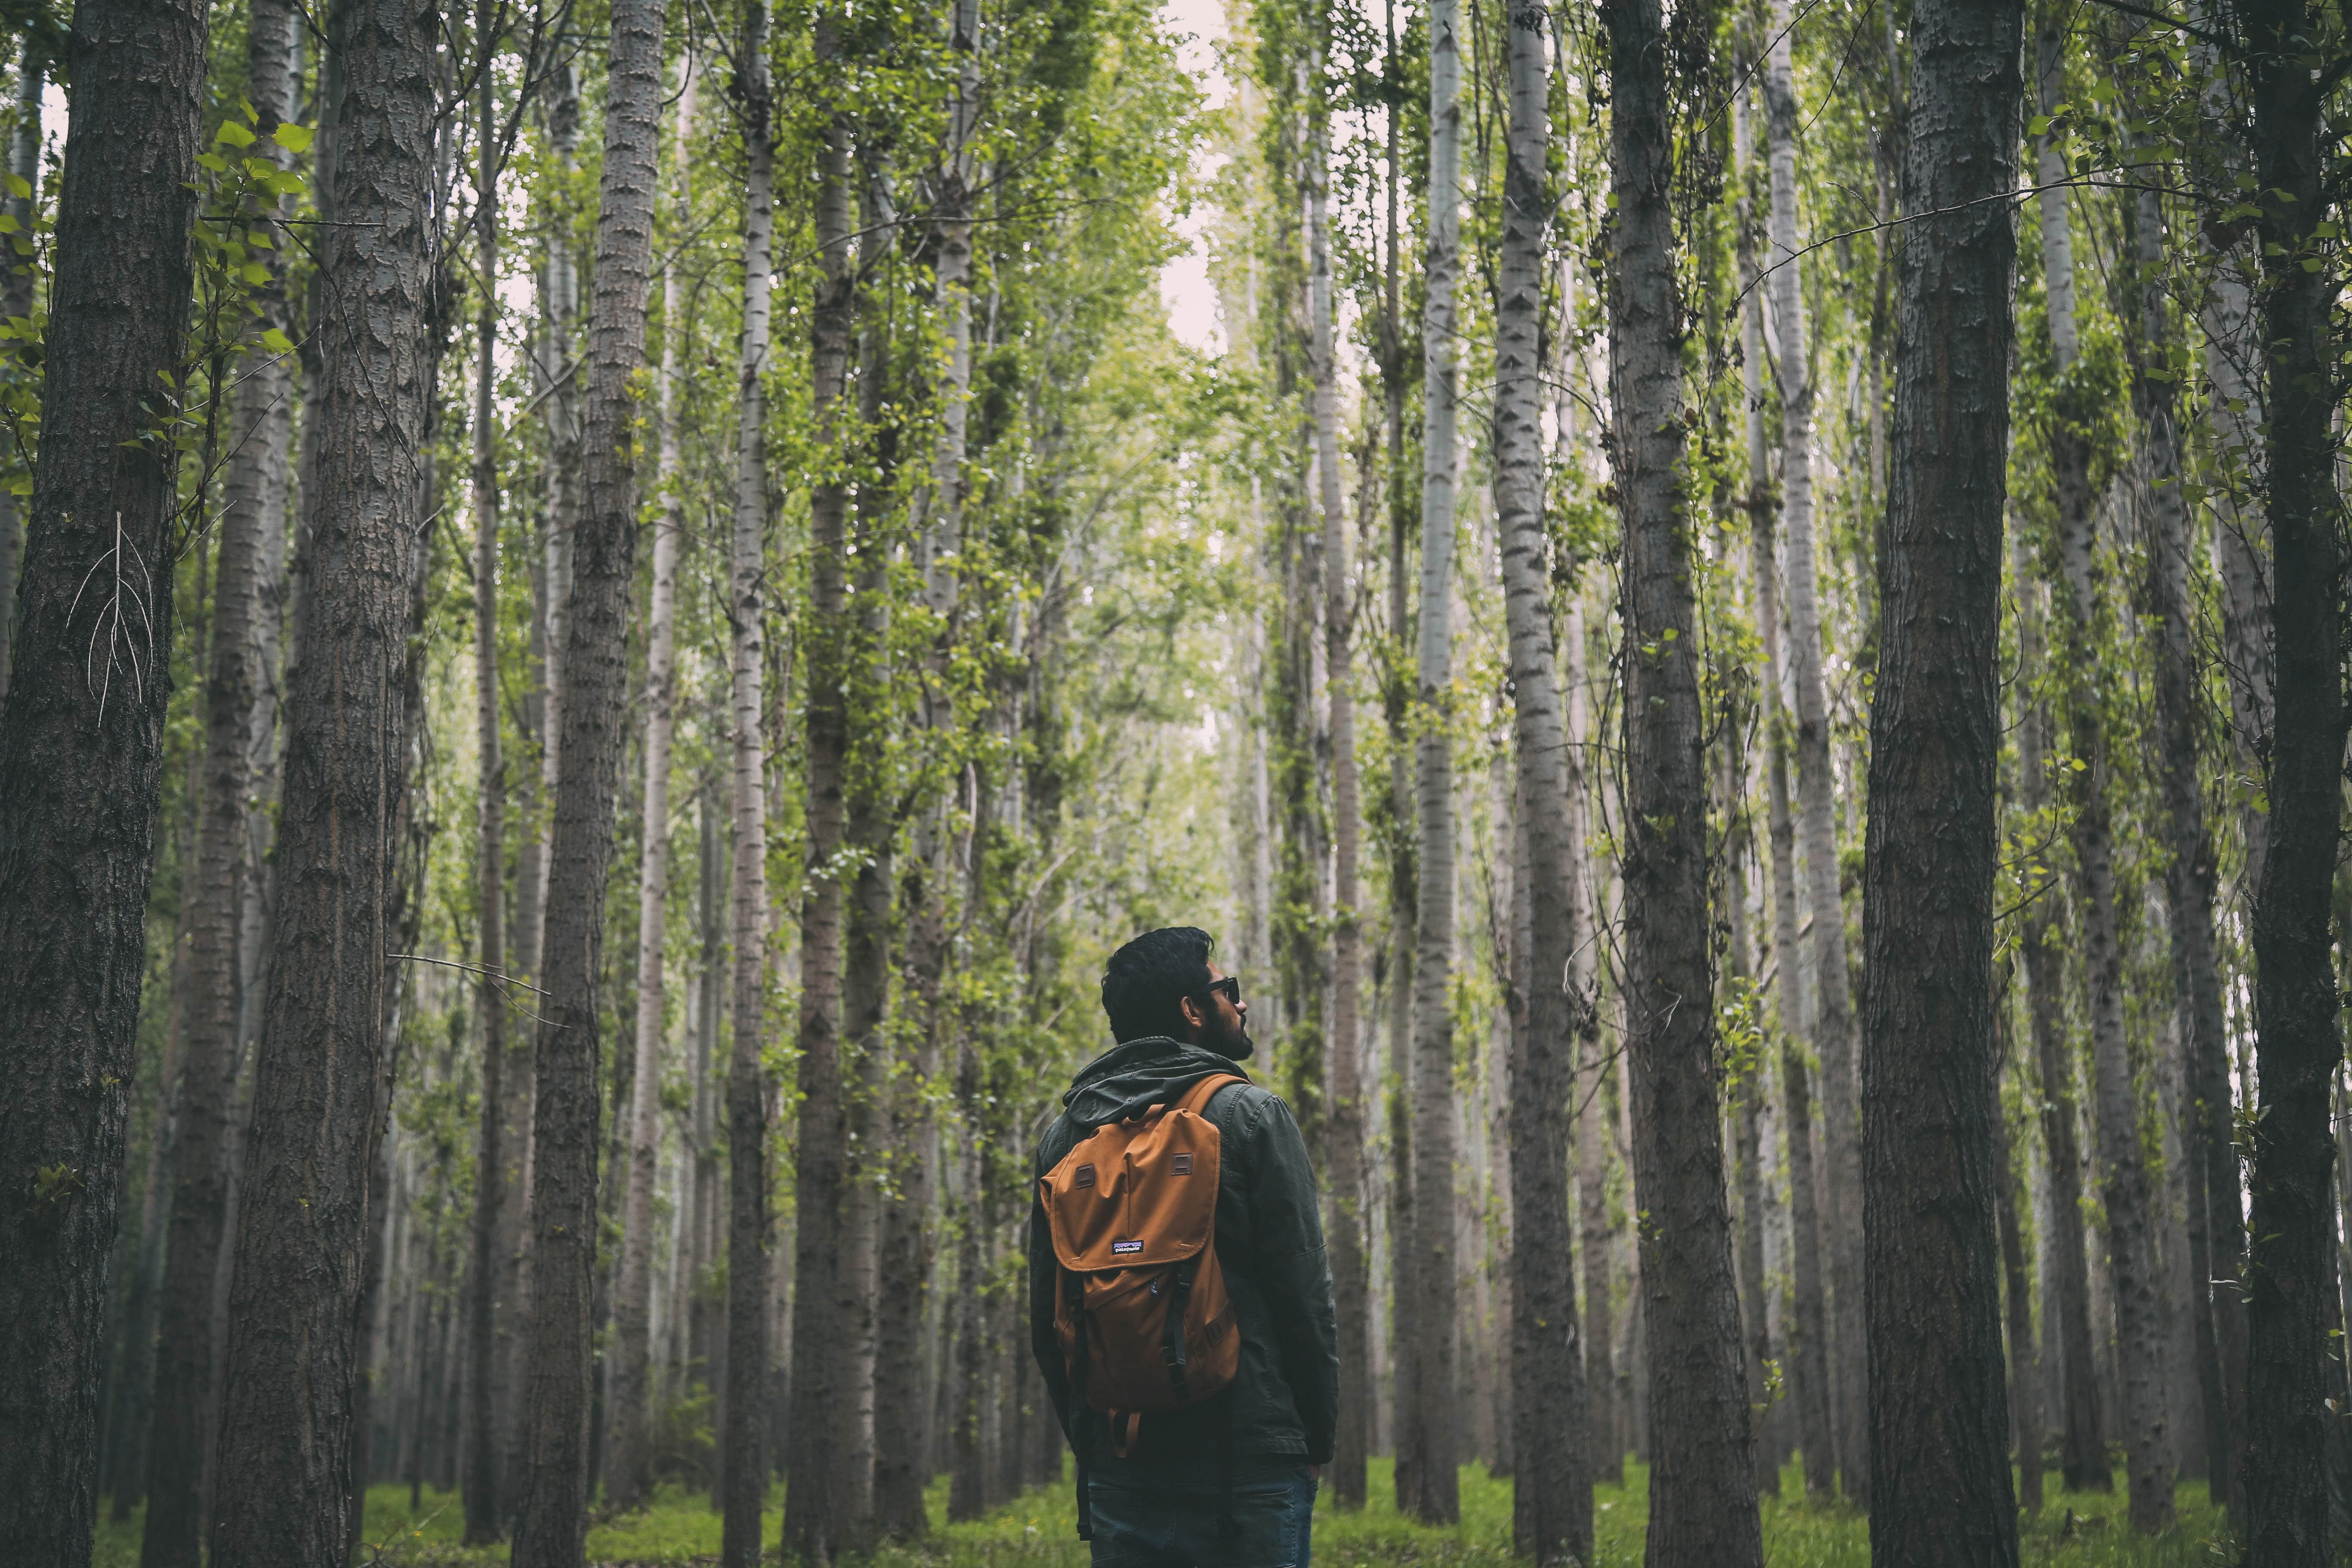
\includegraphics[width=9cm,keepaspectratio]{exploring} \\
    \bigskip
    \inserttitle \\
  \end{center}
\end{frame}

\setbeamertemplate{footline}[myfootline]

\begin{frame}
  \frametitle{Finding your Passion}
  \framesubtitle{Exploring 0 - Finding your Passion}
  \begin{columns}[onlytextwidth]
    \begin{column}{.30\textwidth}
      \begin{figure}
        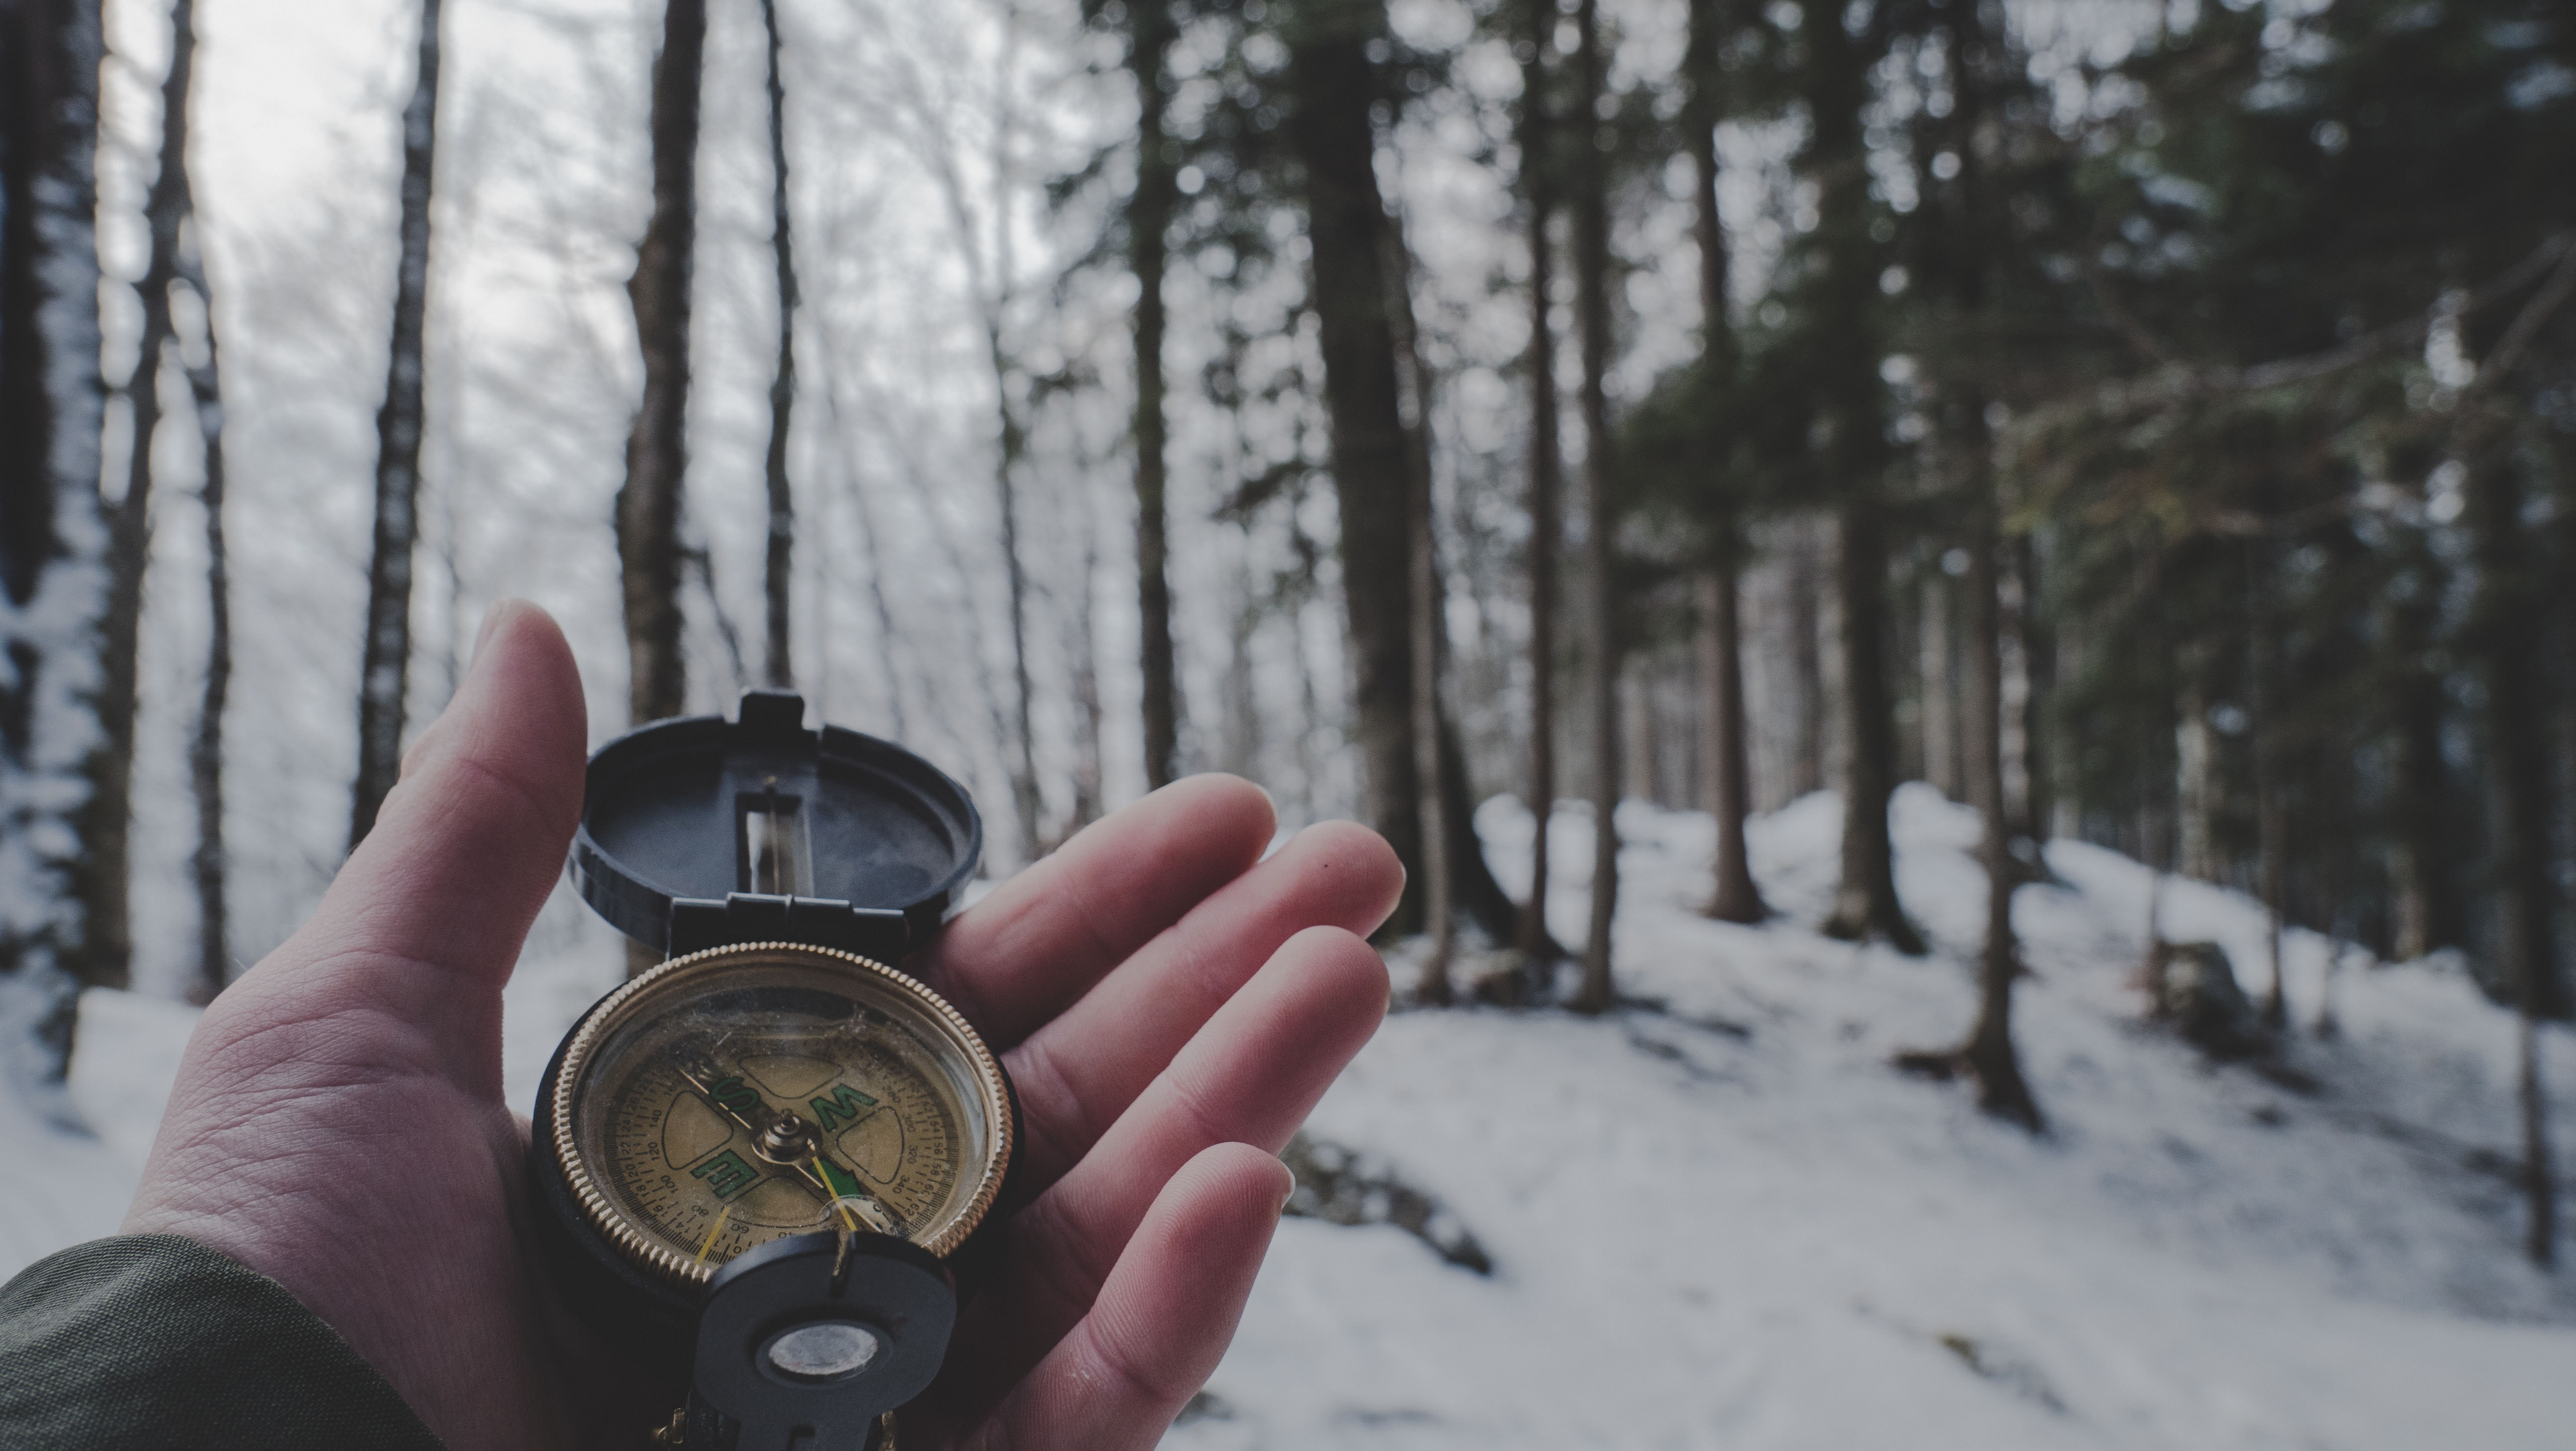
\includegraphics[width=5.5cm,keepaspectratio]{compass}
        \caption{Finding your Way}
      \end{figure}
    \end{column}
    \hfill
    \begin{column}{.60\textwidth}
        \begin{tcolorbox}[title=finding\_your\_passion.log,colback=gray]
          Don't be afraid to join different social groups and try different things.
          If you don't like something don't waste your time and move on to the next thing on your list.
        \end{tcolorbox}
    \end{column}
  \end{columns}
\end{frame}

\begin{frame}
  \frametitle{Opportunity}
  \framesubtitle{Exploring 1 - Opportunity}
  \begin{columns}[onlytextwidth]
    \begin{column}{.30\textwidth}
      \begin{figure}
        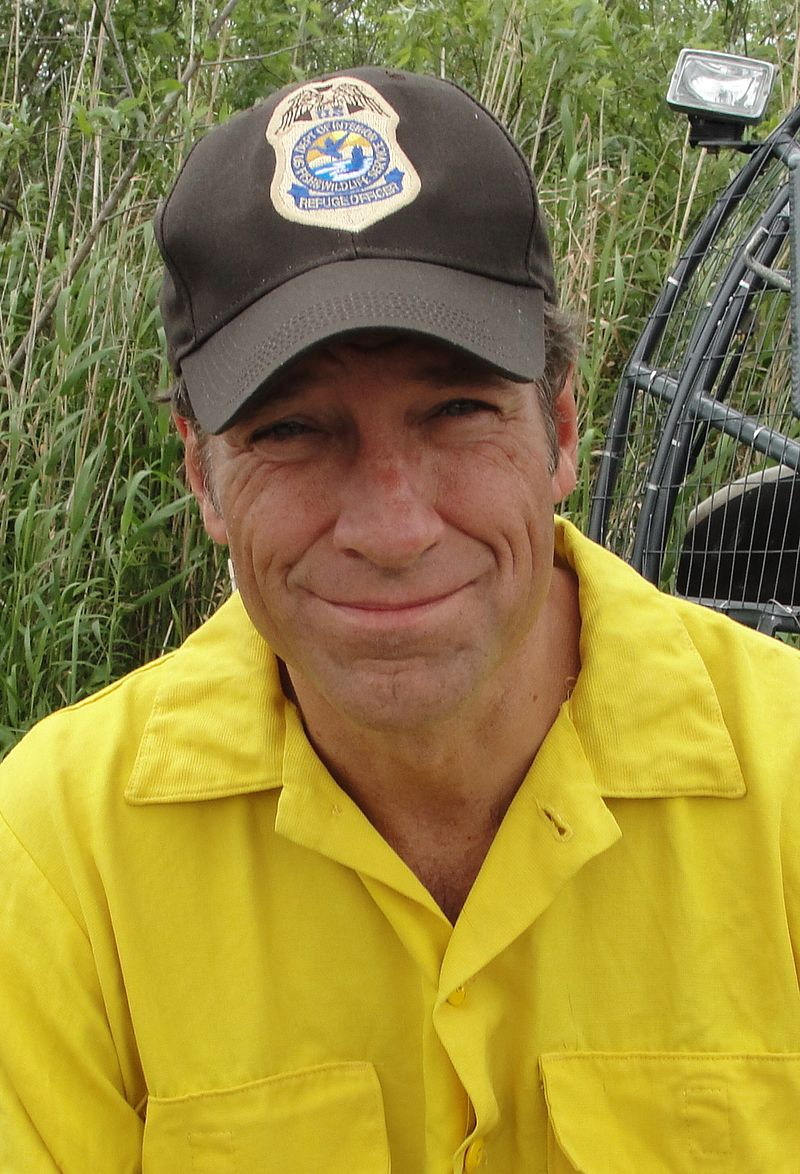
\includegraphics[width=4cm,keepaspectratio]{mike_rowe}
        \caption{Mike Rowe}
      \end{figure}
    \end{column}
    \hfill
    \begin{column}{.60\textwidth}
        \begin{tcolorbox}[title=mike\_rowe.log,colback=gray]
          Take your passion with you, but don't follow it around. Instead, follow opportunity. - Mike Rowe
        \end{tcolorbox}
    \end{column}
  \end{columns}
\end{frame}

\begin{frame}
  \frametitle{Try it Out}
  \framesubtitle{Exploring 2 - Try it Out}
  \begin{columns}[onlytextwidth]
    \begin{column}{.30\textwidth}
      \begin{figure}
        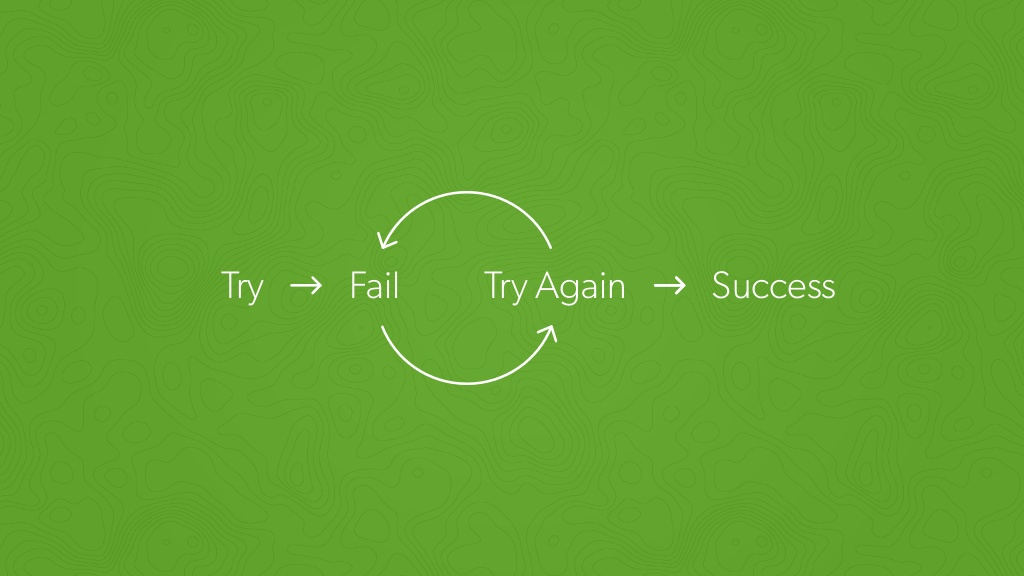
\includegraphics[width=5.5cm,keepaspectratio]{try_fail_success}
        \caption{Road to Success}
      \end{figure}
    \end{column}
    \hfill
    \begin{column}{.60\textwidth}
        \begin{tcolorbox}[title=success.log,colback=gray]
          We are always going to fail when starting out but if you are passionate about it you will try again until you succeed.
        \end{tcolorbox}
    \end{column}
  \end{columns}
\end{frame}

\begin{frame}
  \frametitle{Story Time}
  \framesubtitle{Exploring 3 - Story Time}
  \begin{center}
    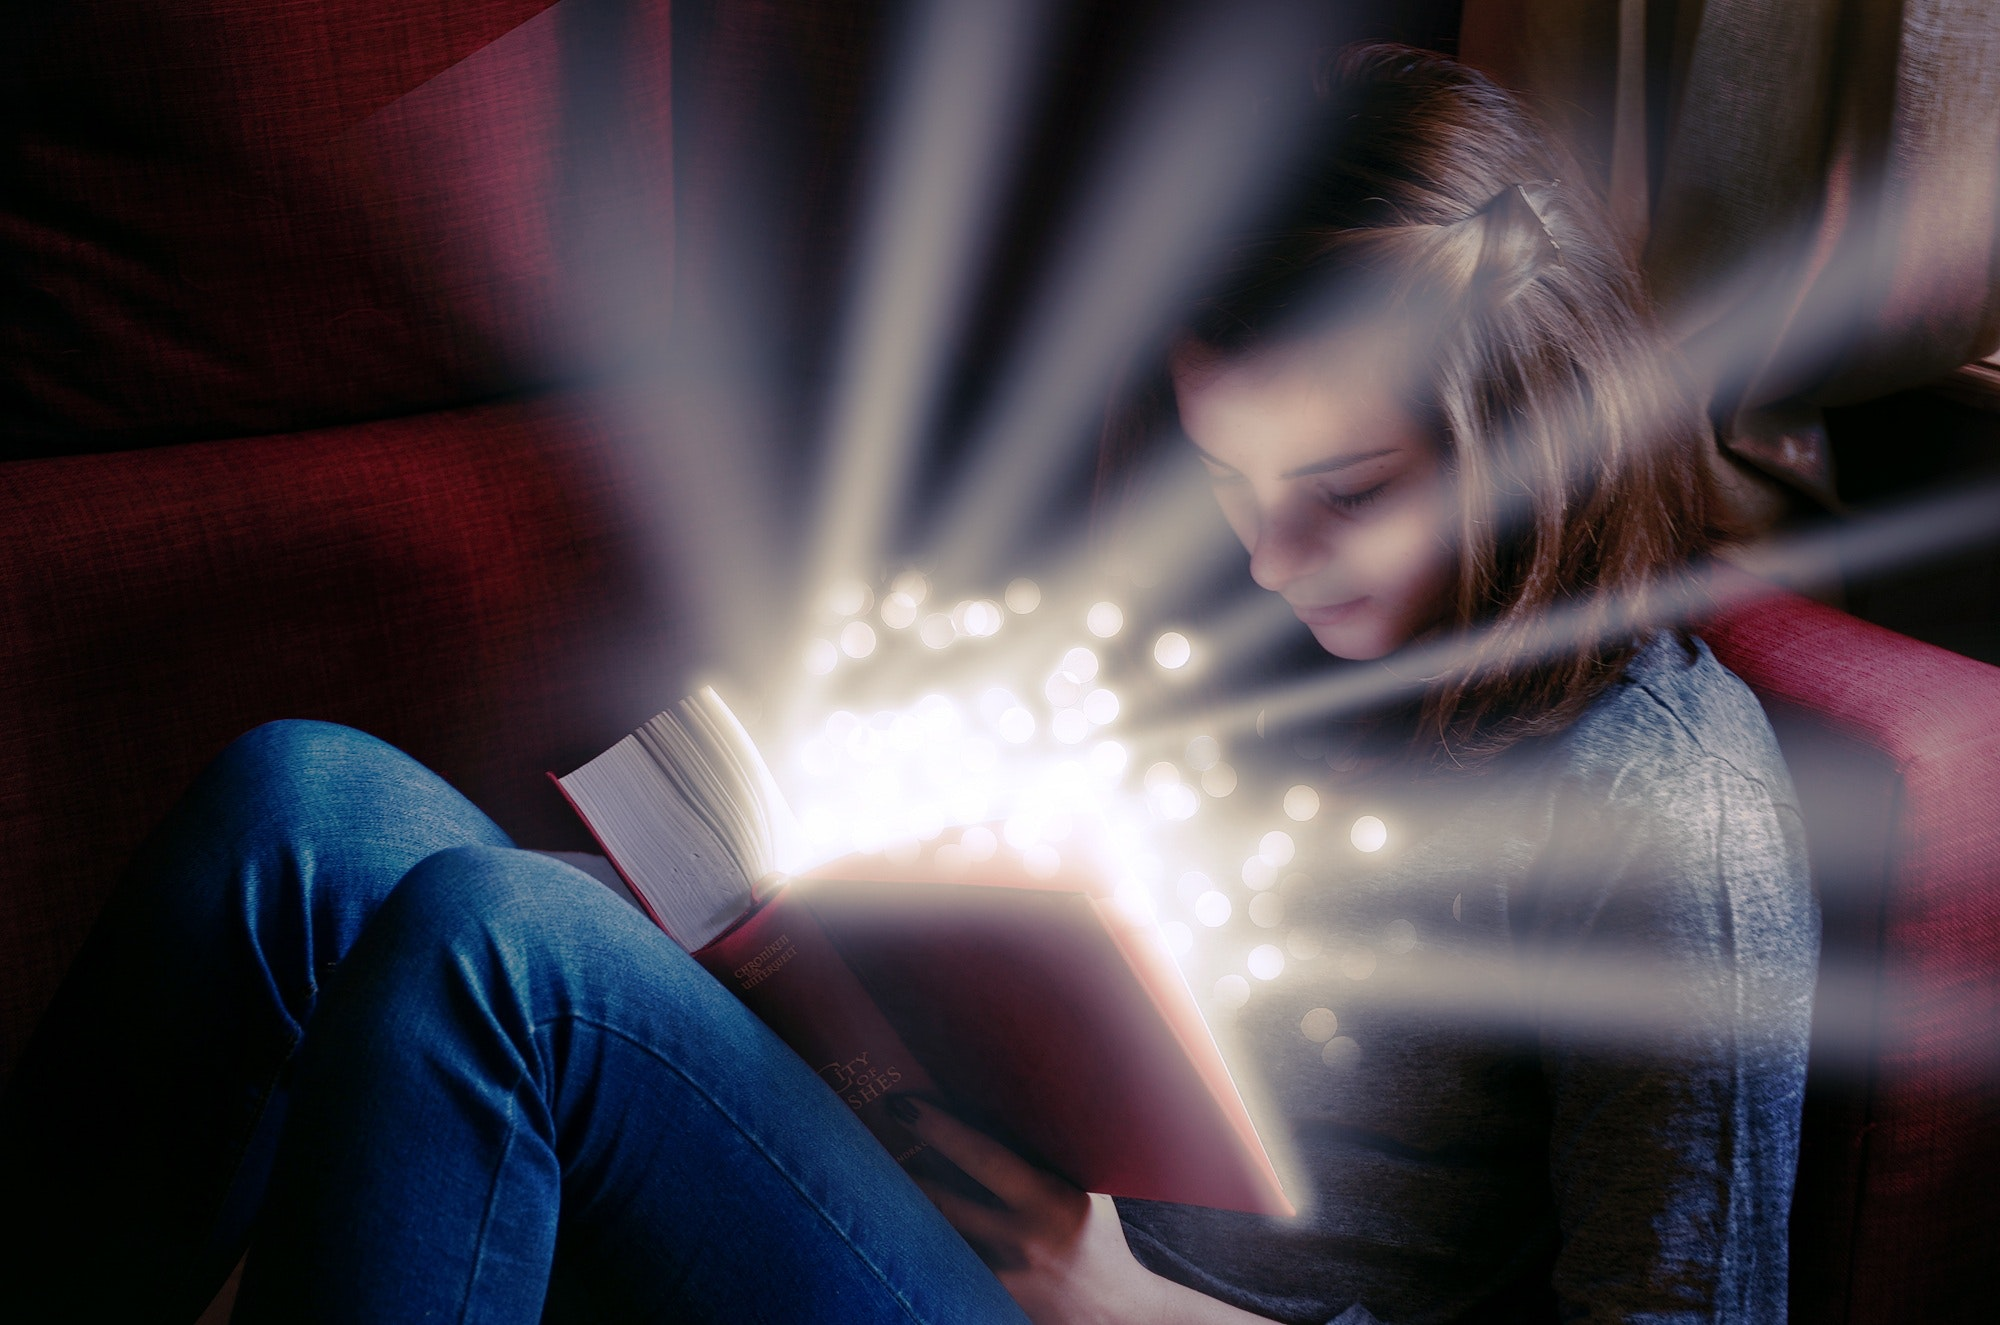
\includegraphics[width=10cm,keepaspectratio]{story_time}
  \end{center}
\end{frame}

\setbeamertemplate{footline}{}

\begin{frame}[t]
  \begin{center}
    \begingroup
    \fontsize{20pt}{20pt}\selectfont
    Learning \\
    \endgroup
    \bigskip
    
\includegraphics[width=9cm,keepaspectratio]{learning} \\
    \bigskip
    \inserttitle \\
  \end{center}
\end{frame}

\setbeamertemplate{footline}[myfootline]

\begin{frame}
  \frametitle{Post Secondary Education}
  \framesubtitle{Learning 0 - Post Secondary Education}
  \begin{columns}[onlytextwidth]
    \begin{column}{.30\textwidth}
      \begin{figure}
        
\includegraphics[width=5.5cm,keepaspectratio]{post_secondary}
        \caption{Post Secondary}
      \end{figure}
    \end{column}
    \hfill
    \begin{column}{.60\textwidth}
        \begin{tcolorbox}[title=success.log,colback=gray]
          It's not always required to go to post secondary education to get the skills you need to be successful. Post secondary education does look great on a resume but keep in mind most employers are looking for someone who can do the job as well.
        \end{tcolorbox}
    \end{column}
  \end{columns}
\end{frame}

\begin{frame}
  \frametitle{Online Education}
  \framesubtitle{Learning 1 - Online Education}
  \begin{columns}[onlytextwidth]
    \begin{column}{.30\textwidth}
      \begin{figure}
        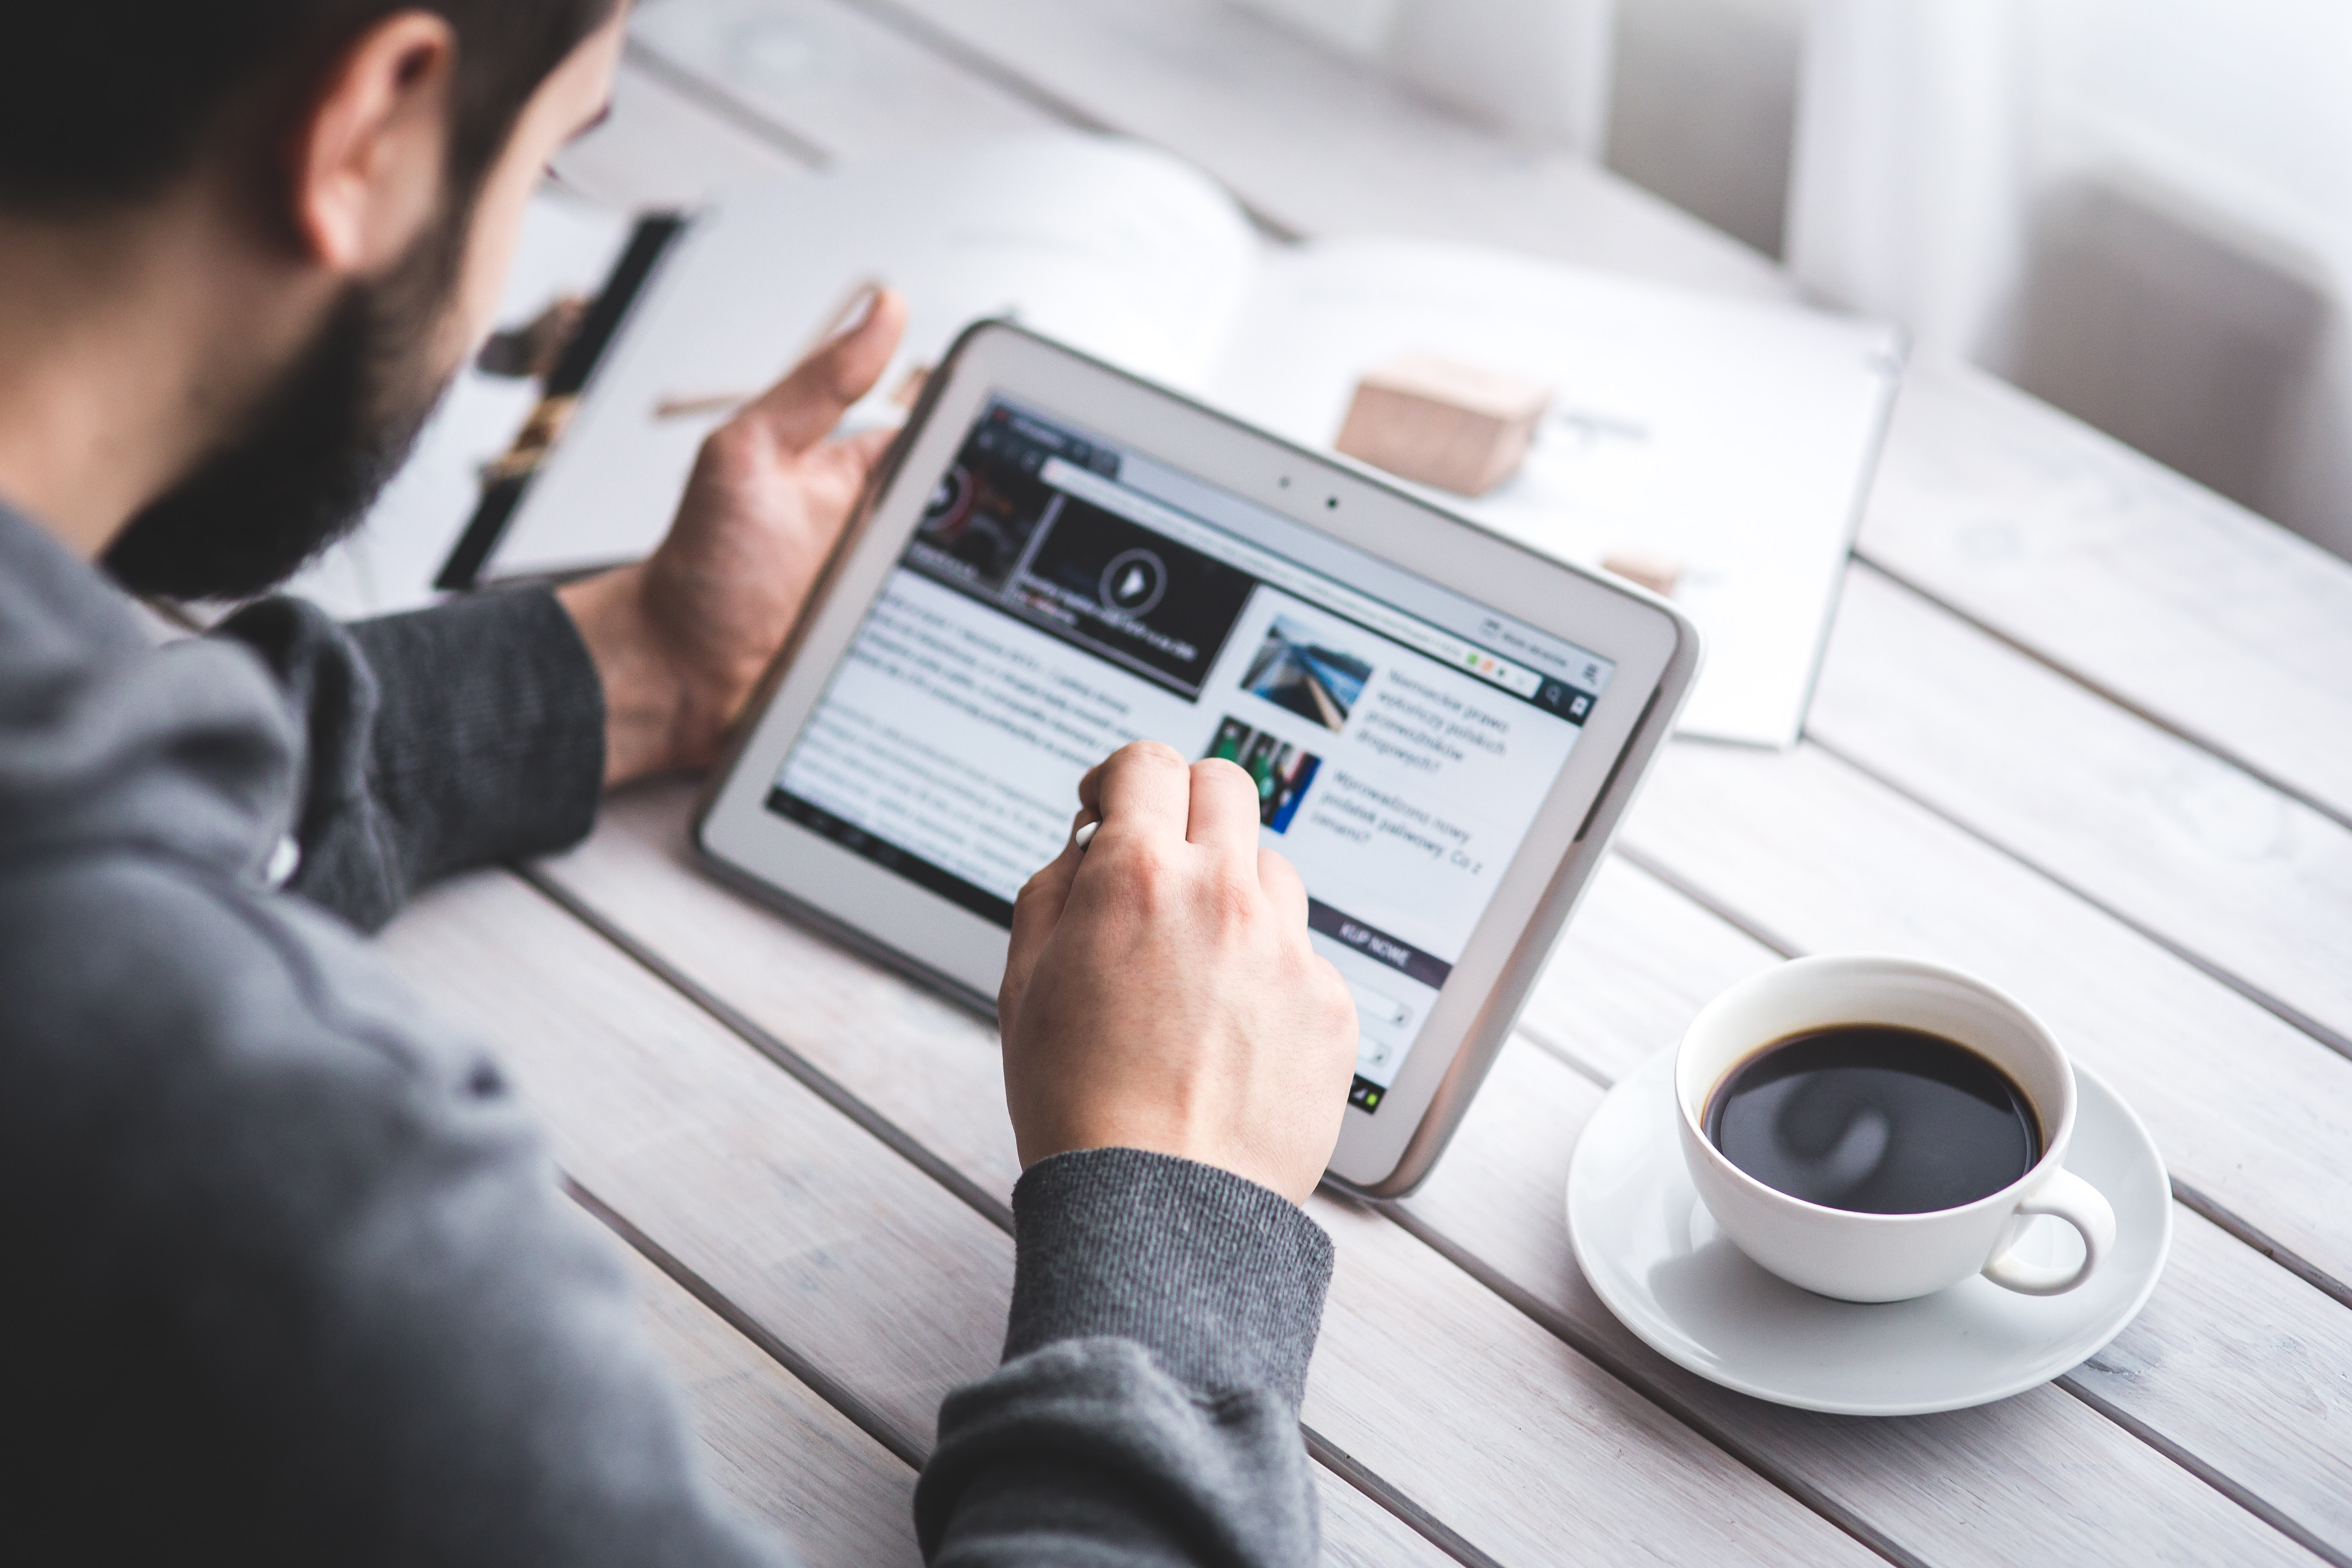
\includegraphics[width=5.5cm,keepaspectratio]{online}
        \caption{Post Secondary}
      \end{figure}
    \end{column}
    \hfill
    \begin{column}{.60\textwidth}
        \begin{tcolorbox}[title=online.log,colback=gray]
          Years ago you had to go the the library which almost never had books on teaching you a given field. Times have now changed where you have the world of knowledge at your fingertips. Taking advantage of this will only make you a stronger asset to potential employers.
        \end{tcolorbox}
    \end{column}
  \end{columns}
\end{frame}

\begin{frame}
  \frametitle{Mentor}
  \framesubtitle{Learning 2 - Mentor}
  \begin{columns}[onlytextwidth]
    \begin{column}{.30\textwidth}
      \begin{figure}
        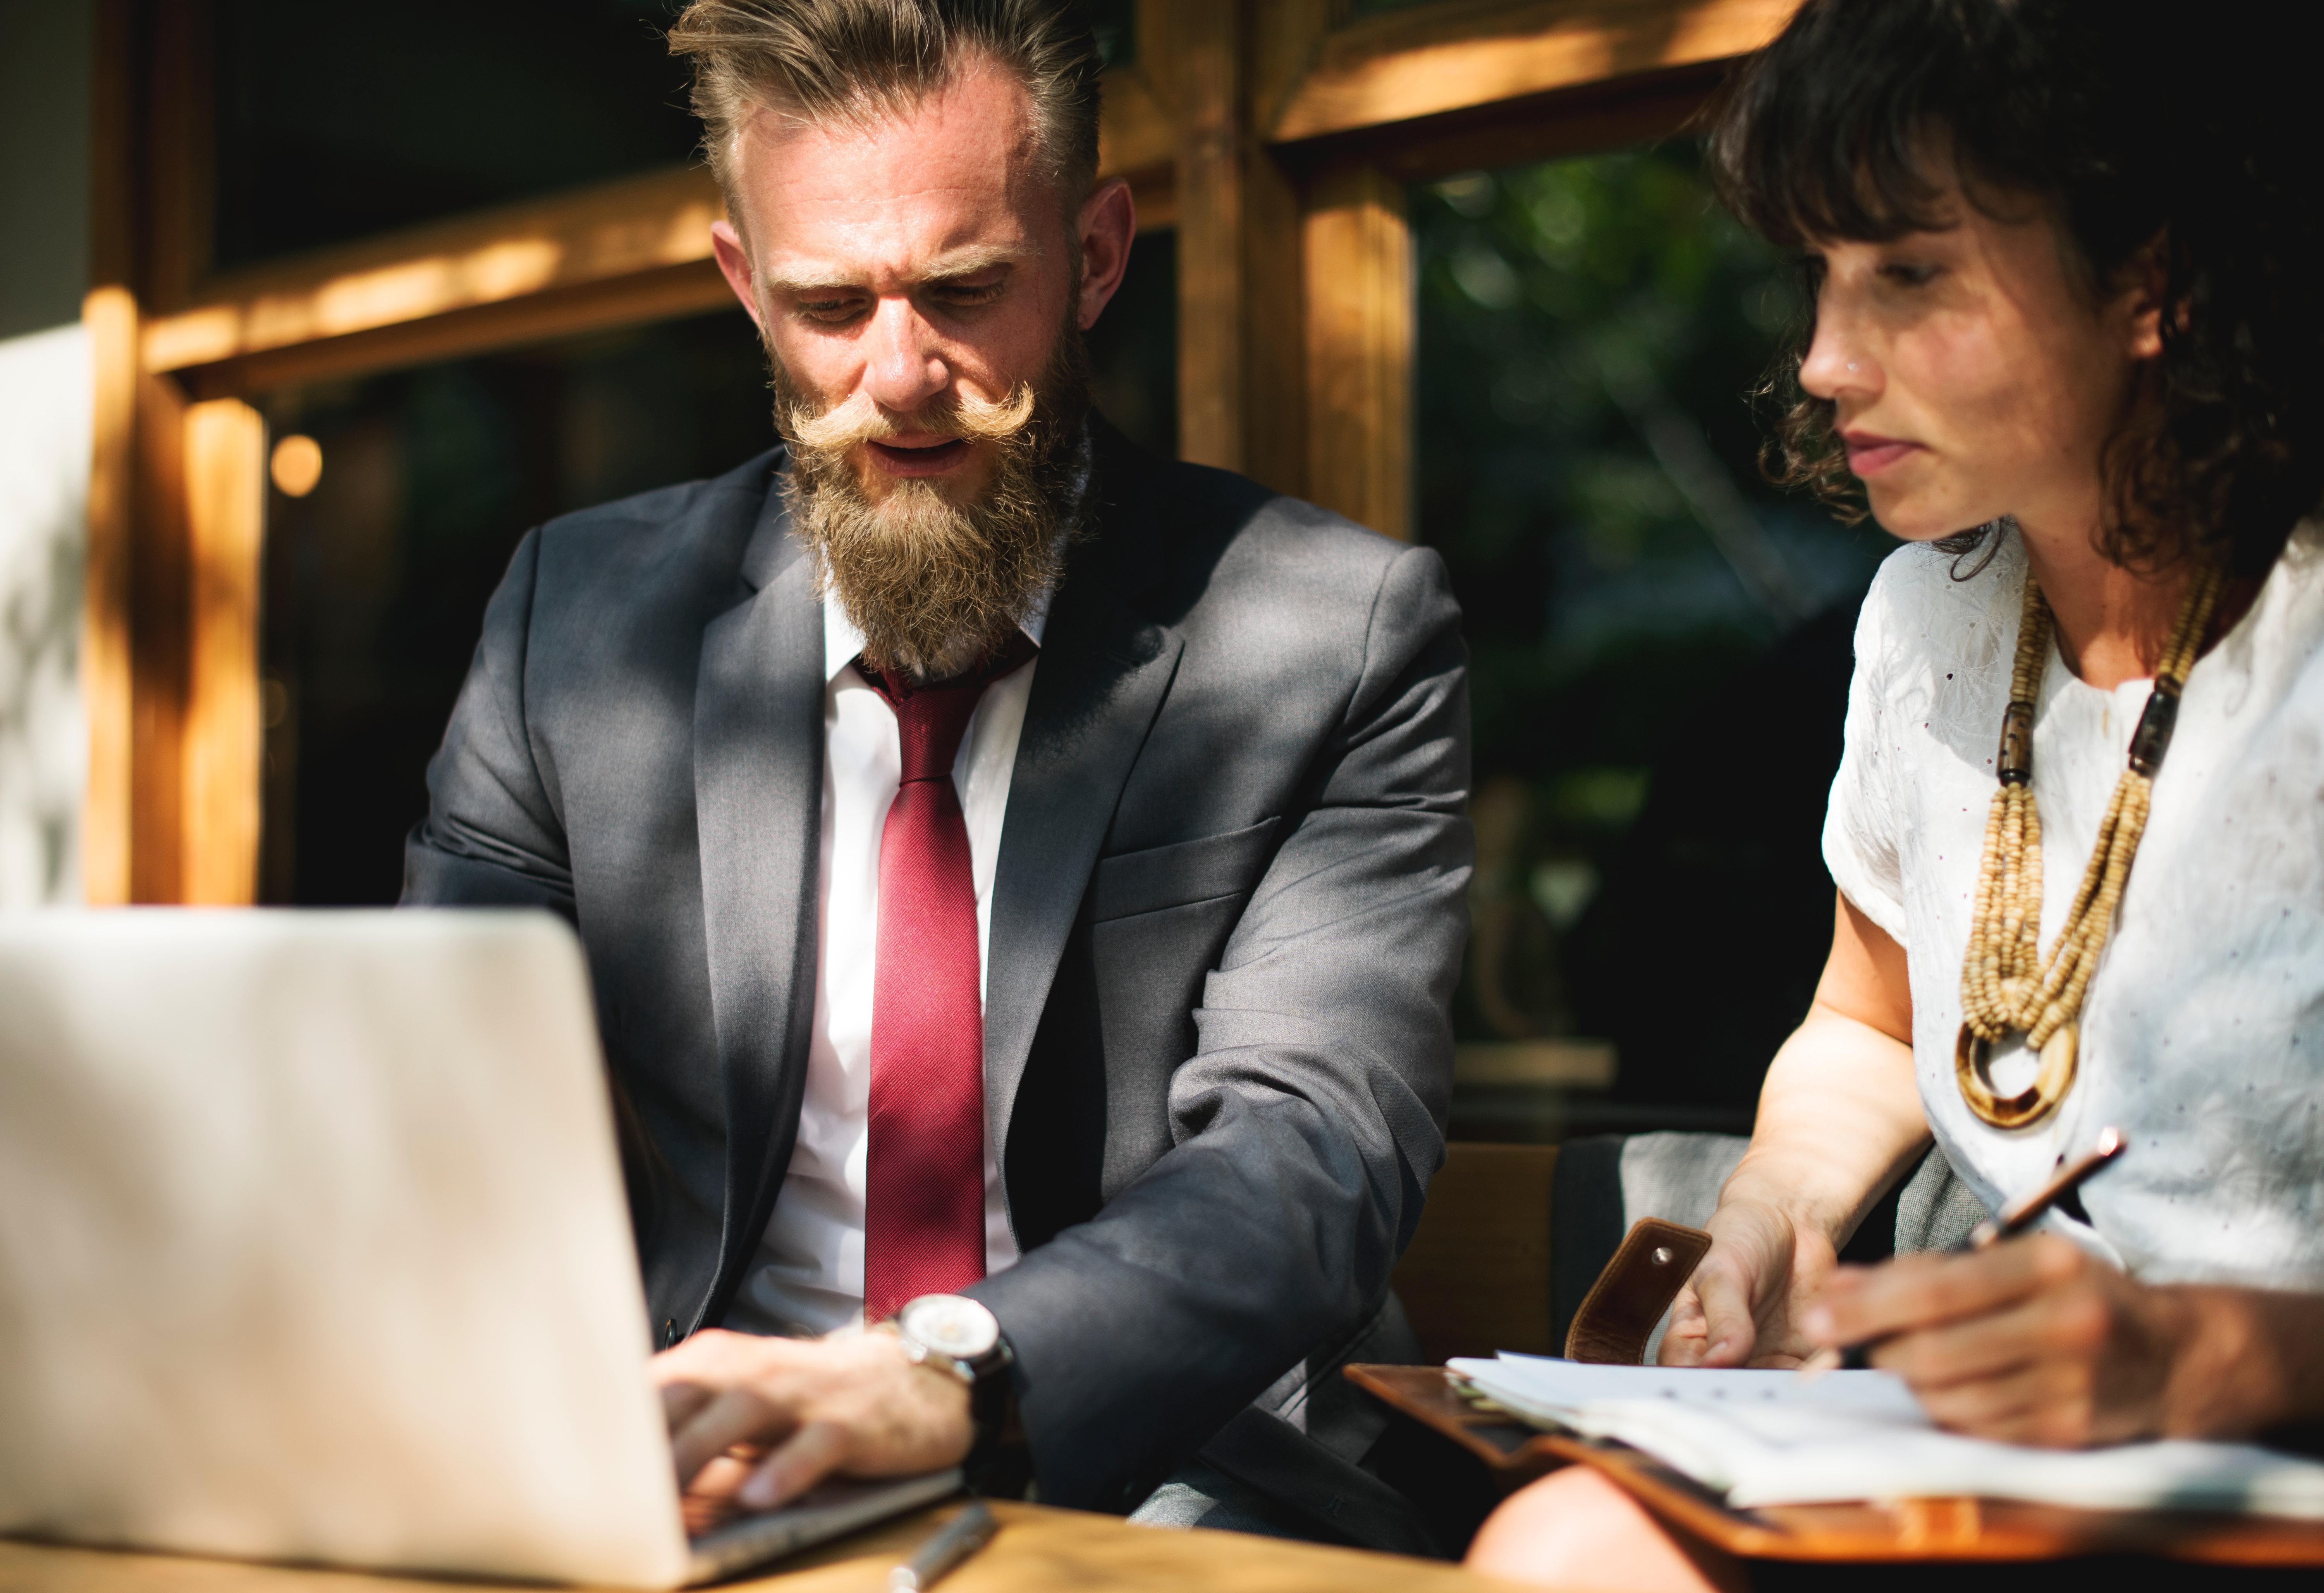
\includegraphics[width=5.5cm,keepaspectratio]{mentor}
        \caption{Mentor}
      \end{figure}
    \end{column}
    \hfill
    \begin{column}{.60\textwidth}
        \begin{tcolorbox}[title=mentor.log,colback=gray]
          Sometimes you can get lucky enough to find a mentor in your area if you network enough. They can help you navigate a more streamlined path to success than if you do it alone.
        \end{tcolorbox}
    \end{column}
  \end{columns}
\end{frame}

\begin{frame}
  \frametitle{Story Time}
  \framesubtitle{Learning 3 - Story Time}
  \begin{center}
    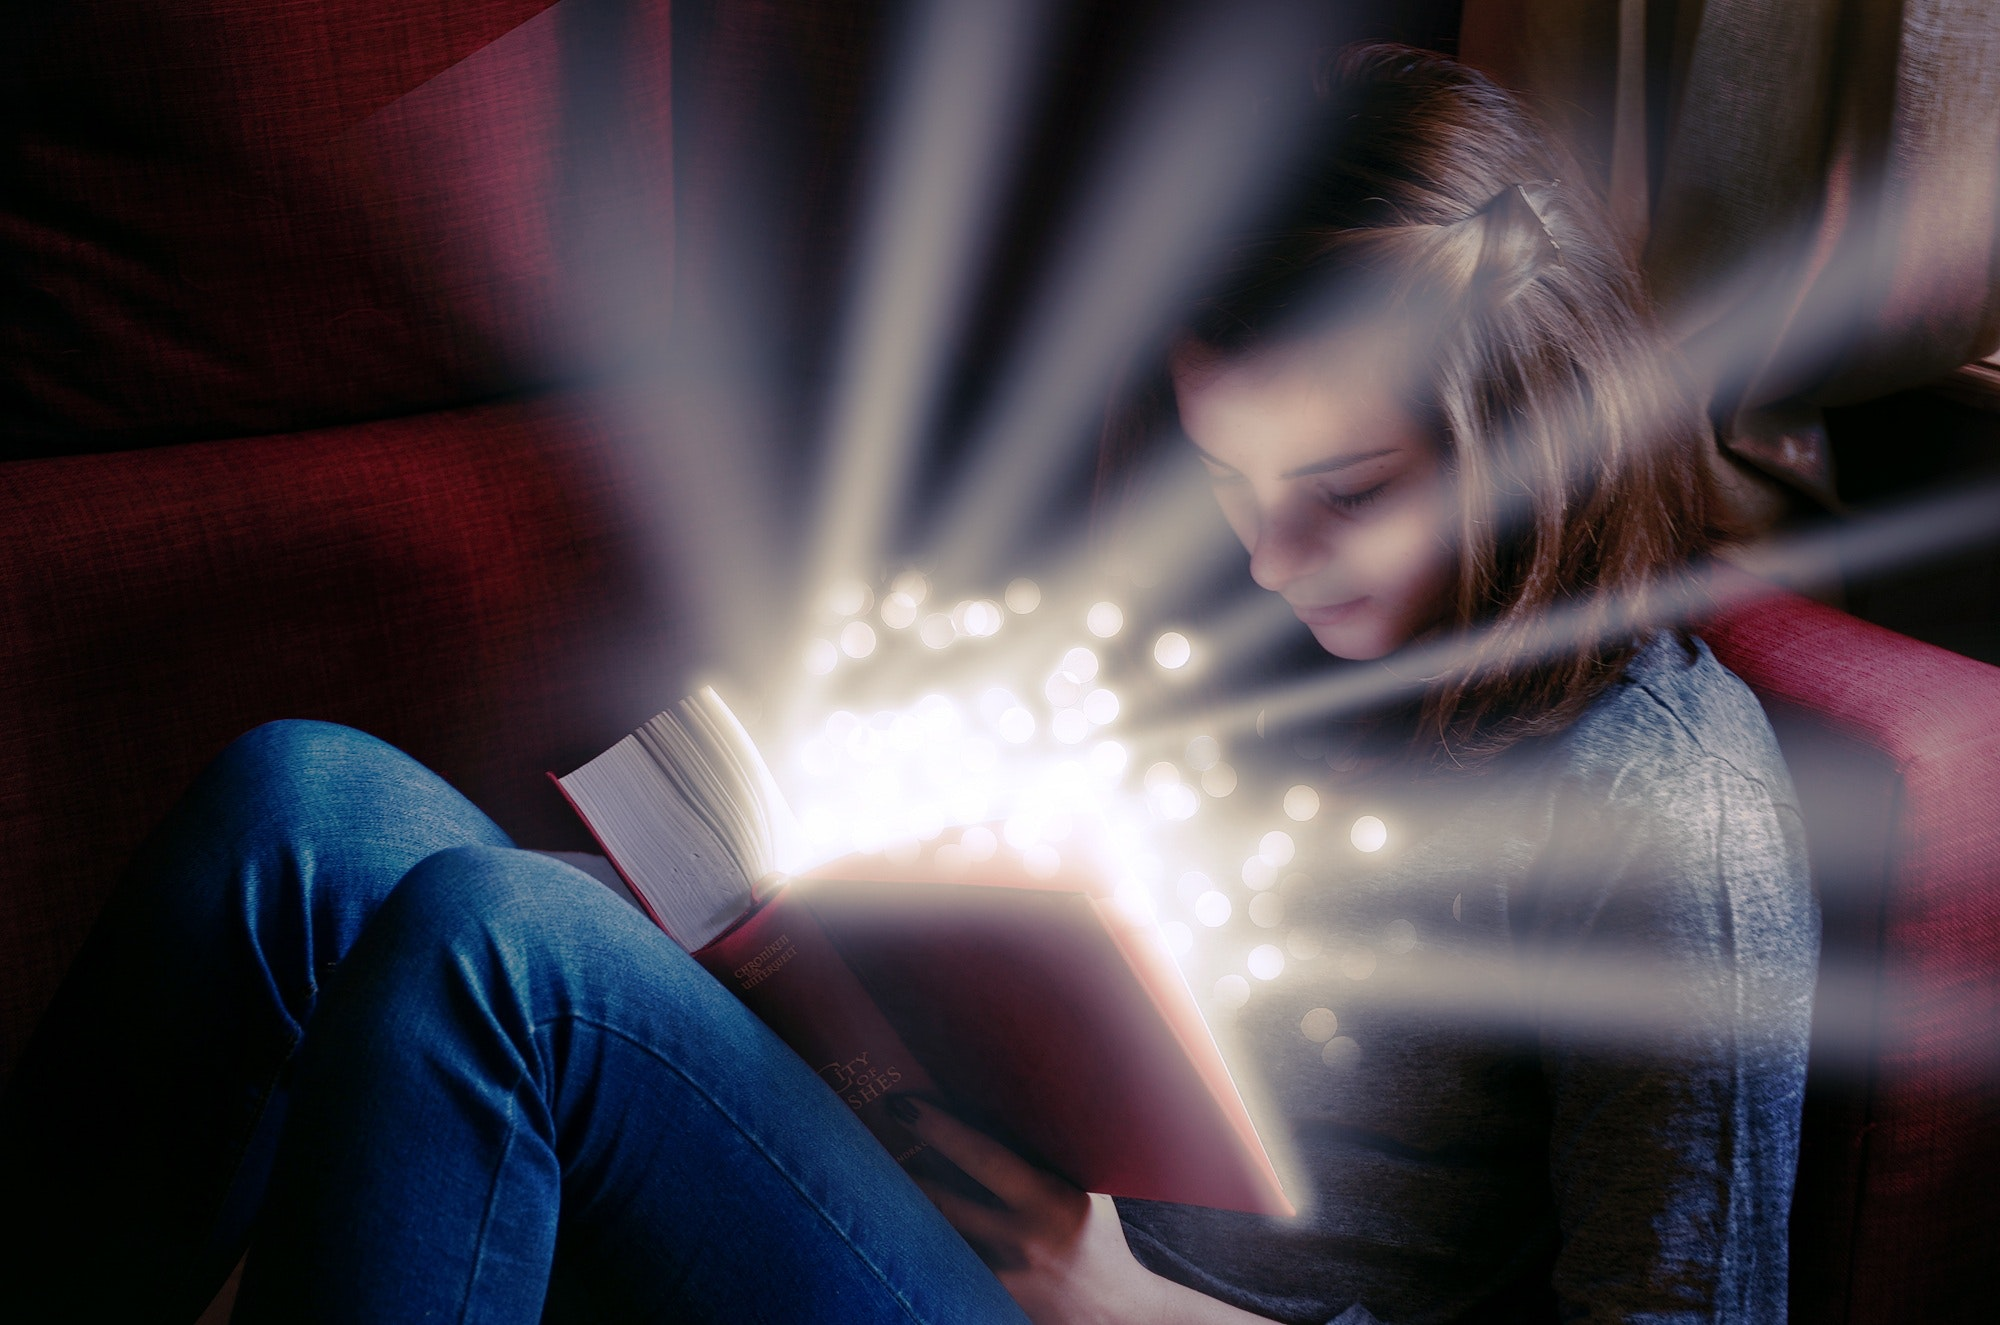
\includegraphics[width=10cm,keepaspectratio]{story_time}
  \end{center}
\end{frame}

\setbeamertemplate{footline}{}

\begin{frame}[t]
  \begin{center}
    \begingroup
    \fontsize{20pt}{20pt}\selectfont
    Showing Value \\
    \endgroup
    \bigskip
    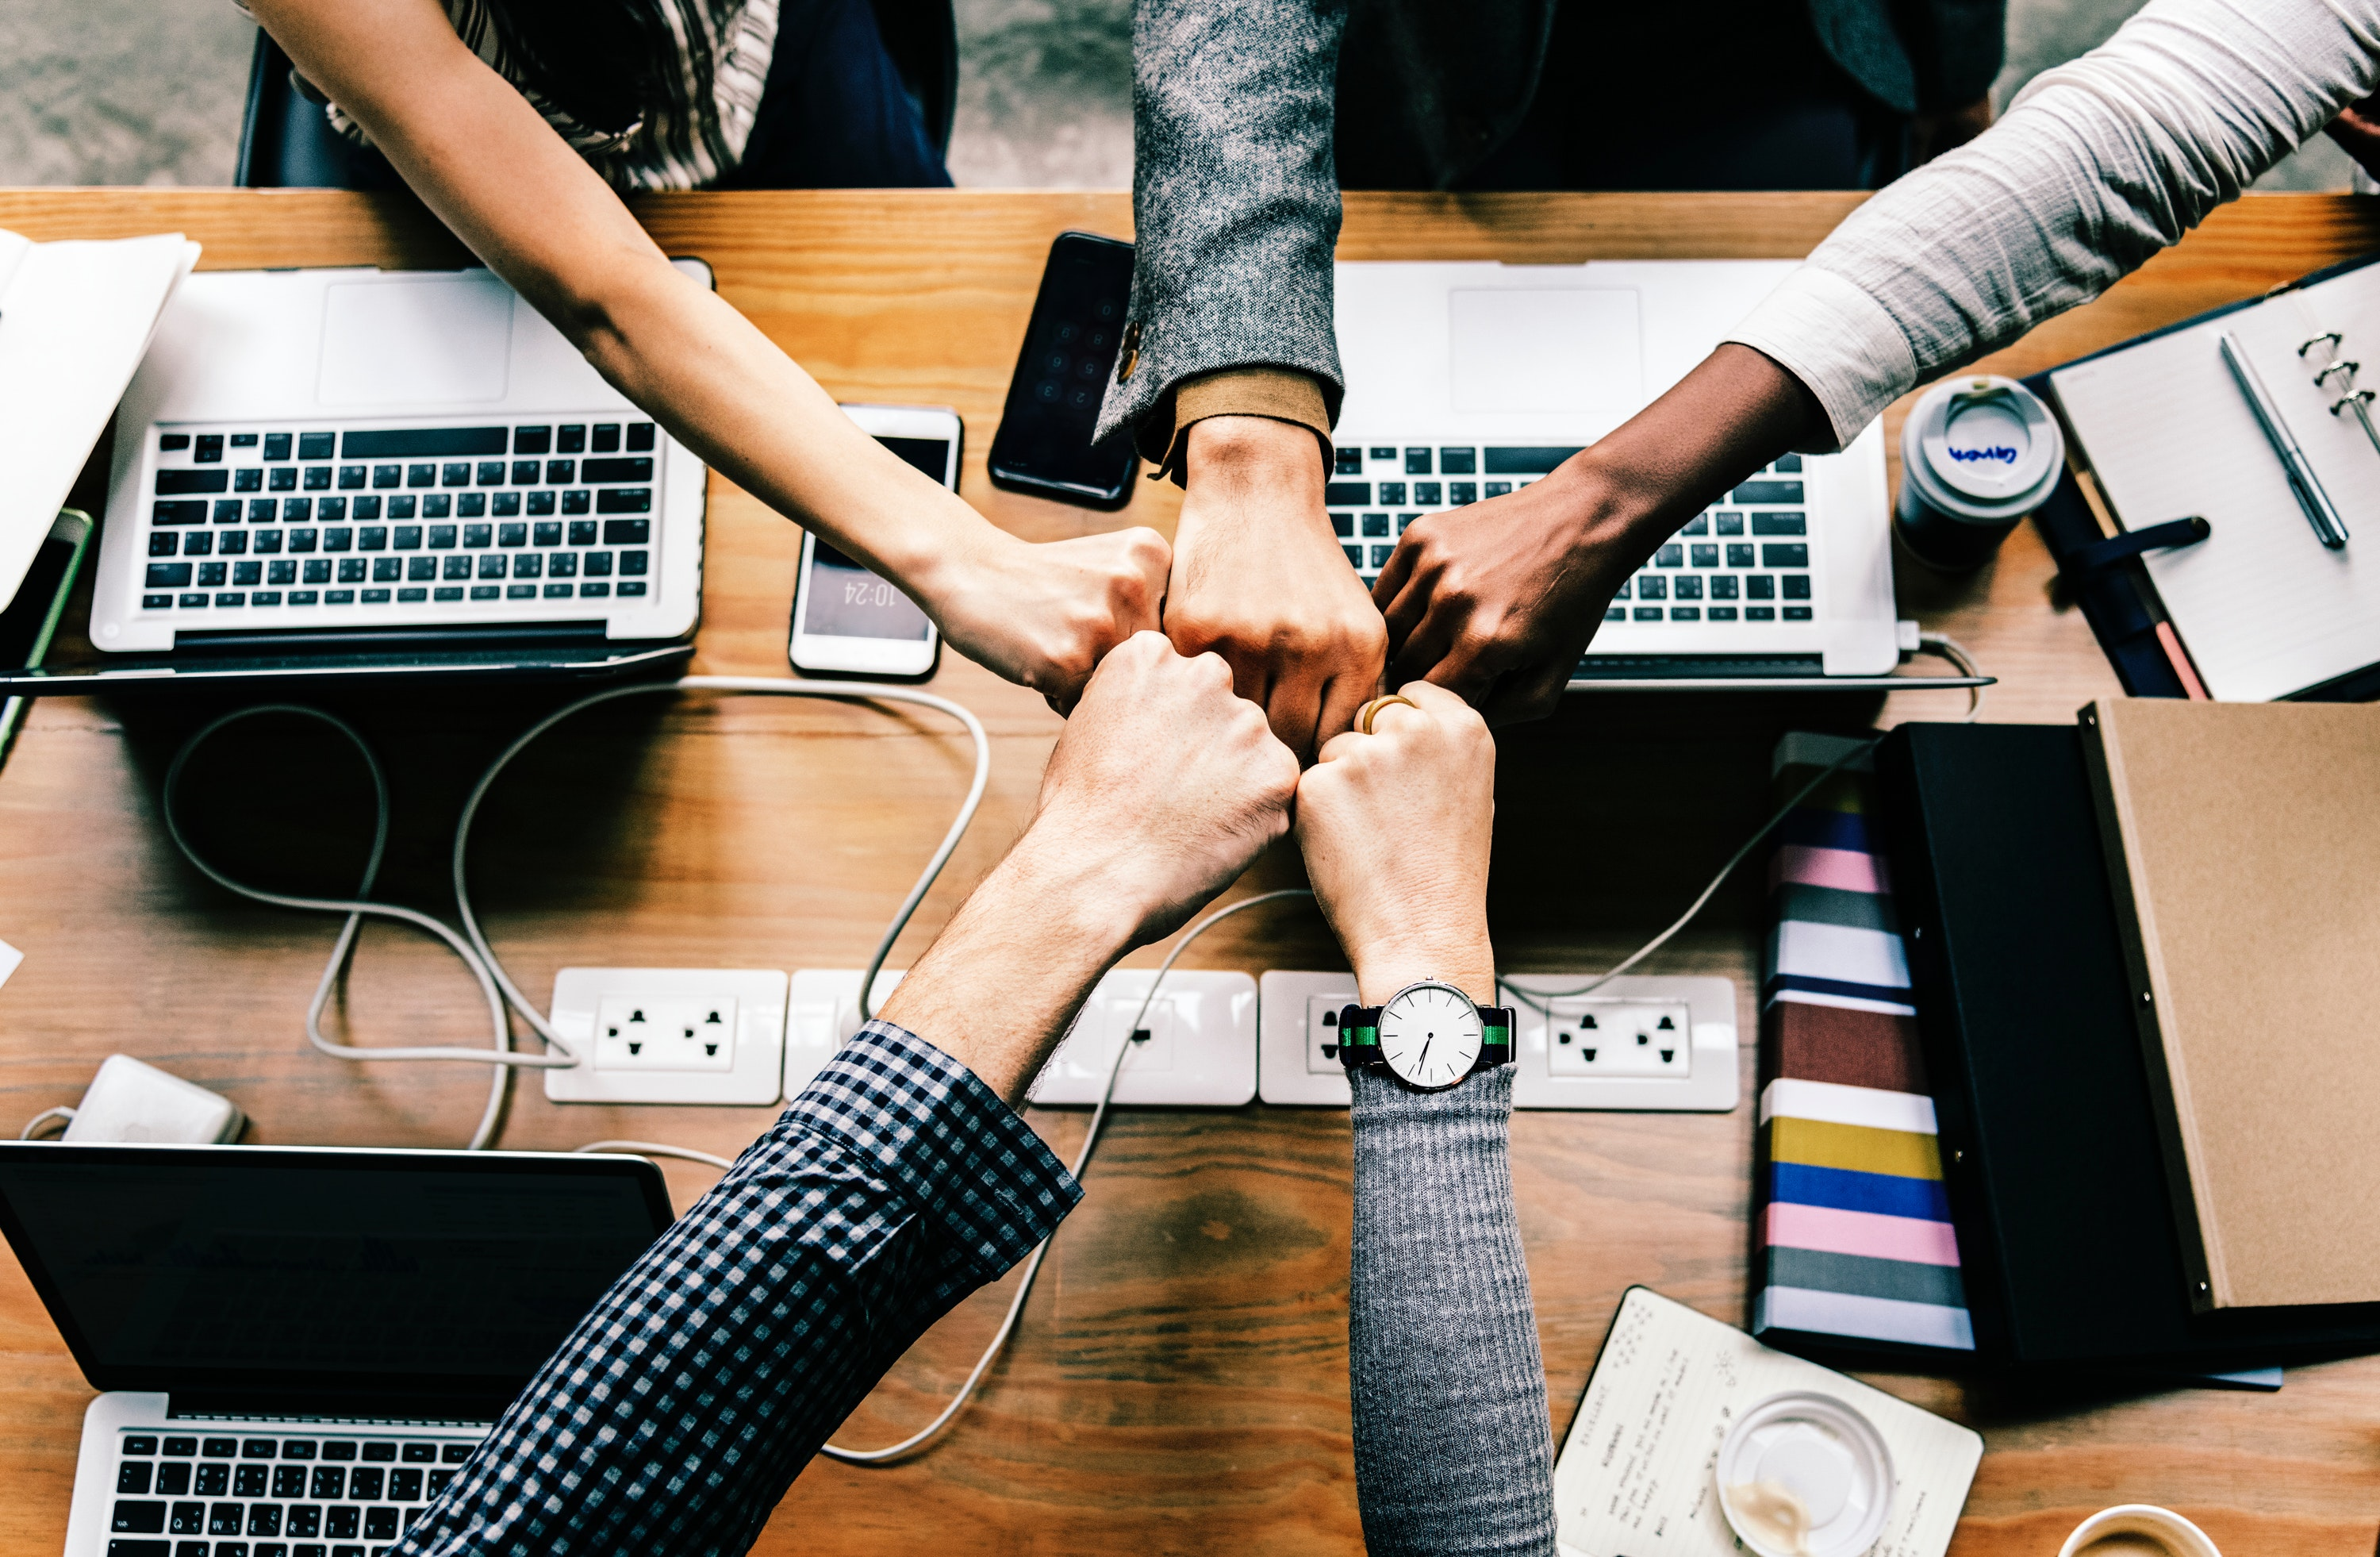
\includegraphics[width=9cm,keepaspectratio]{value} \\
    \bigskip
    \inserttitle \\
  \end{center}
\end{frame}

\setbeamertemplate{footline}[myfootline]

\begin{frame}
  \frametitle{Resume}
  \framesubtitle{Showing Value 0 - Resume}
  \begin{columns}[onlytextwidth]
    \begin{column}{.30\textwidth}
      \begin{figure}
        \includegraphics[width=5.5cm,keepaspectratio]{resume}
        \caption{Resume}
      \end{figure}
    \end{column}
    \hfill
    \begin{column}{.60\textwidth}
        \begin{tcolorbox}[title=resume.log,colback=gray]
          Have a solid resume that not only shows your skills related to the job your are applying for but also links to examples of your work. Employers love to see what you are capable of as it allows them to make better decisions about someones capabilities.
        \end{tcolorbox}
    \end{column}
  \end{columns}
\end{frame}

\begin{frame}
  \frametitle{Social Media}
  \framesubtitle{Showing Value 1 - Social Media}
  \begin{columns}[onlytextwidth]
    \begin{column}{.30\textwidth}
      \begin{figure}
        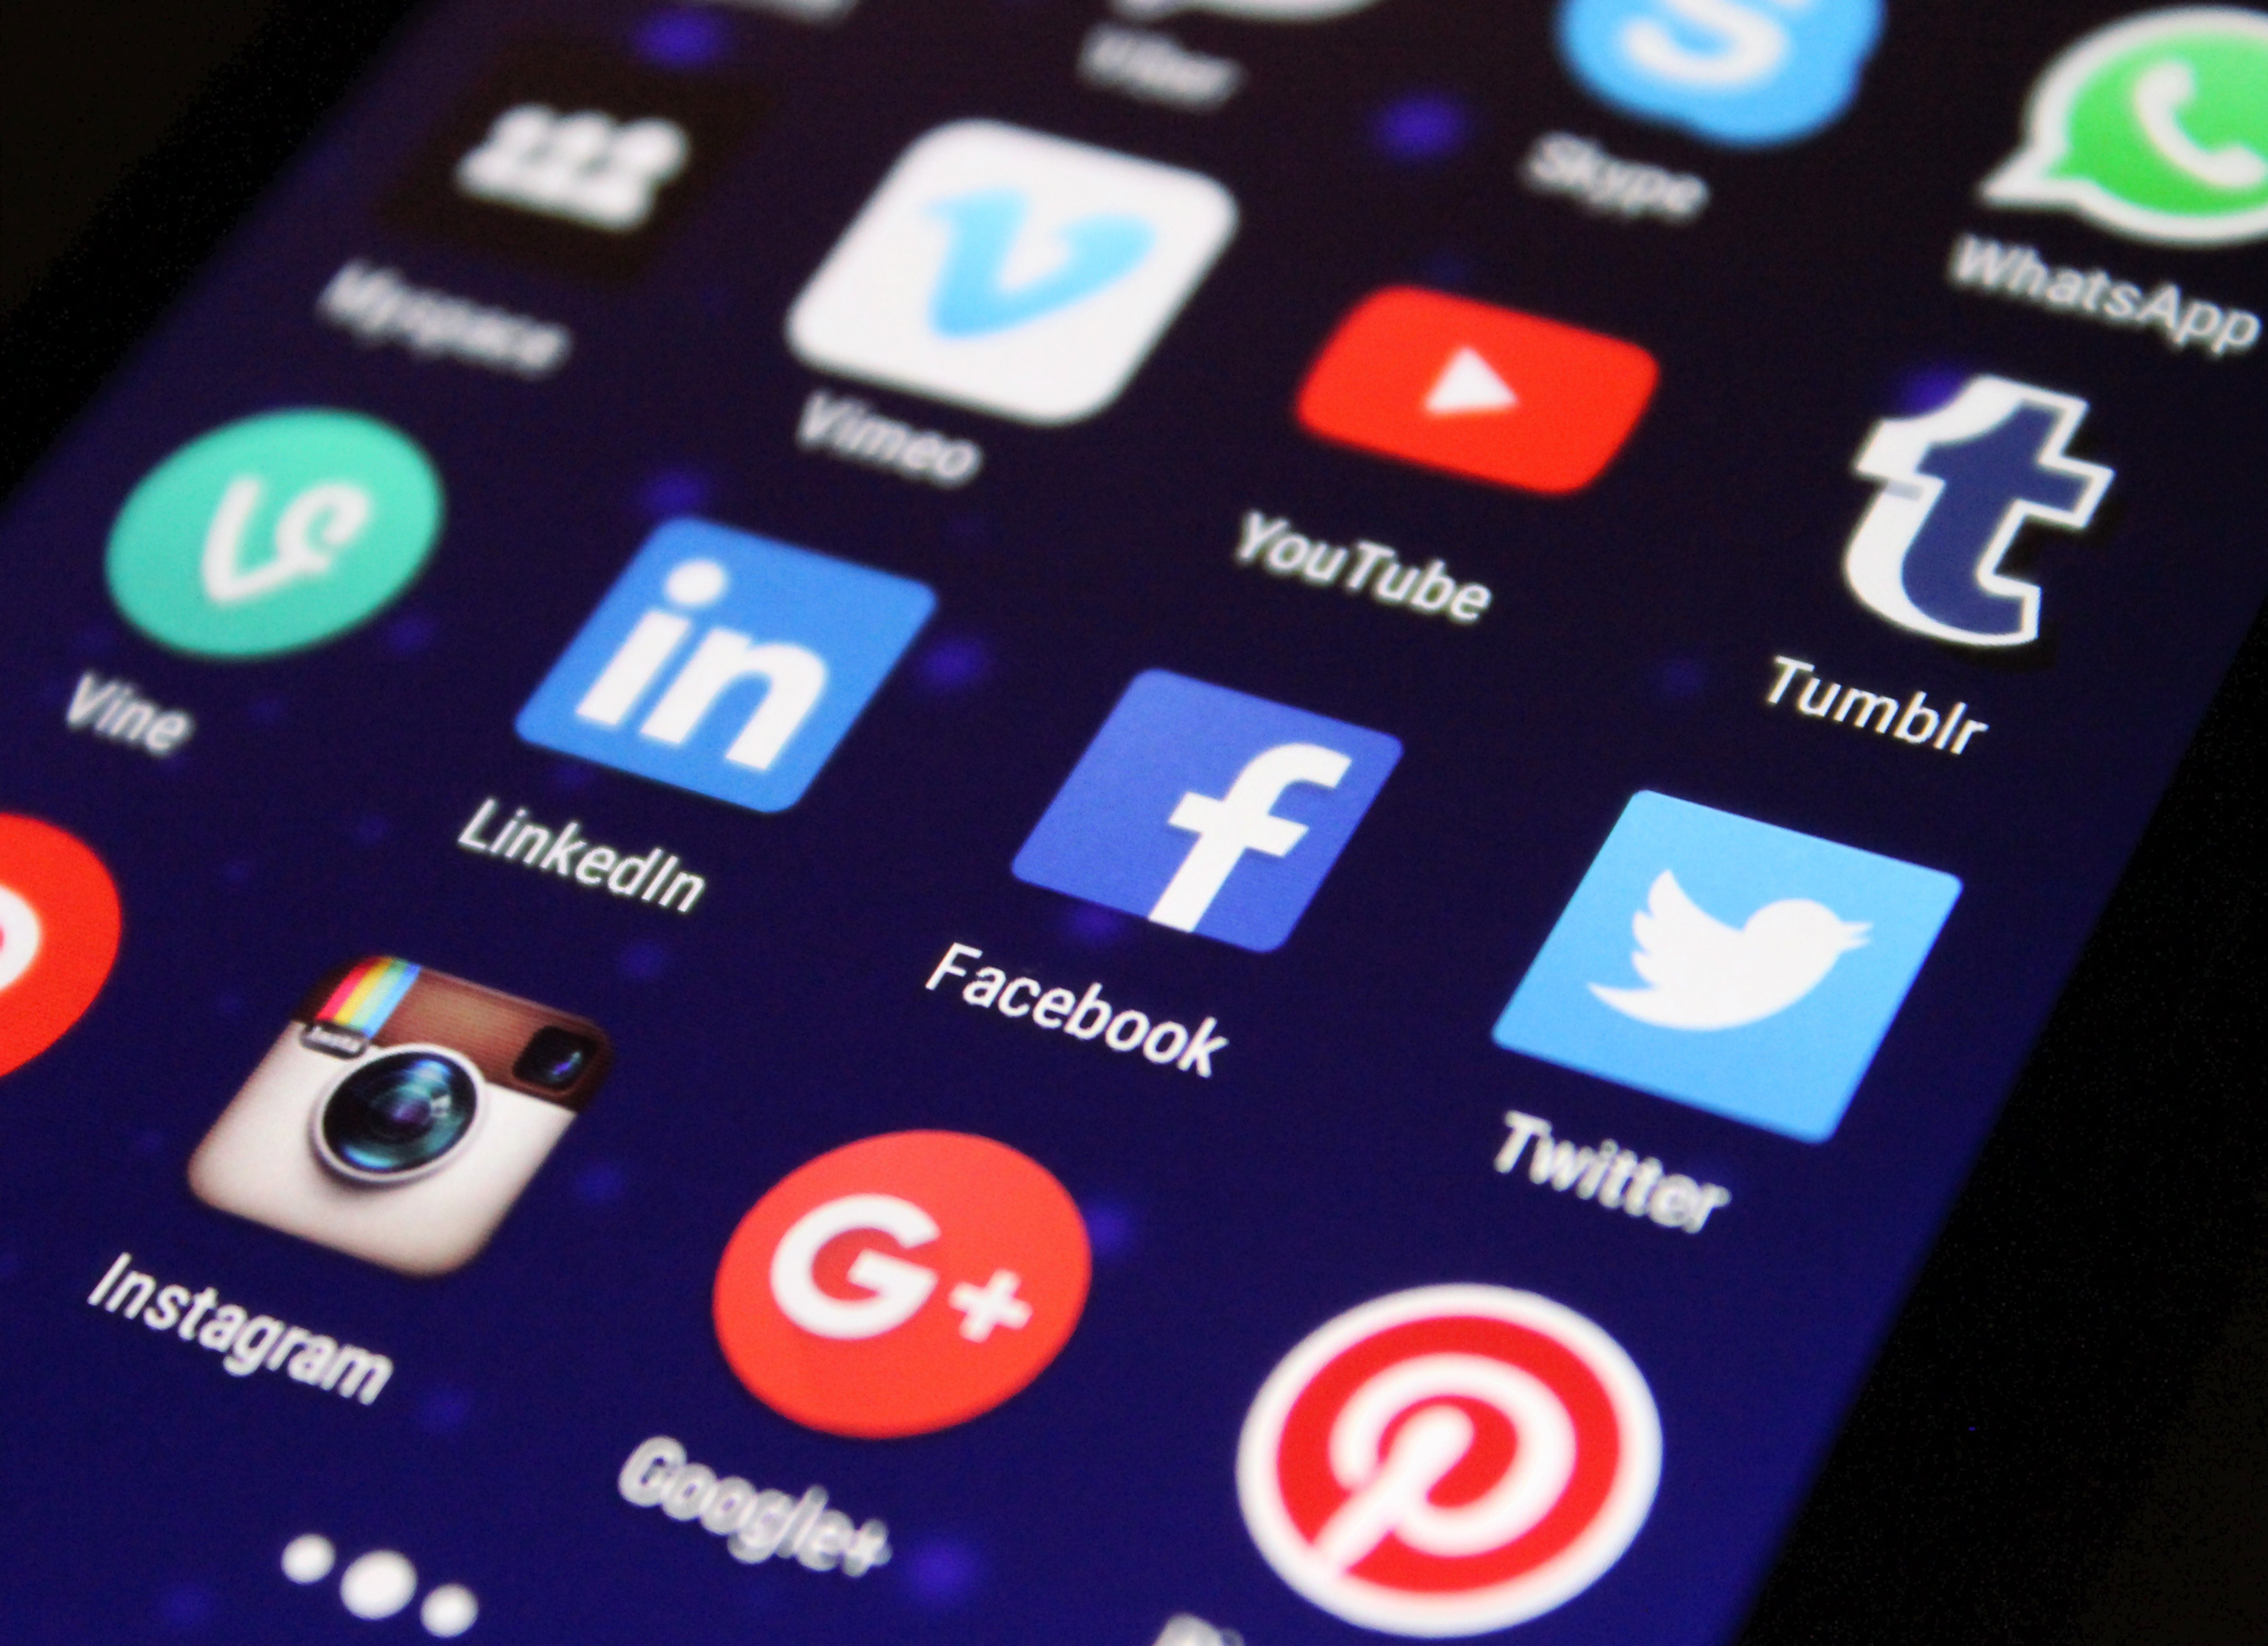
\includegraphics[width=5.5cm,keepaspectratio]{social_media}
        \caption{Social Media}
      \end{figure}
    \end{column}
    \hfill
    \begin{column}{.60\textwidth}
        \begin{tcolorbox}[title=social\_media.log,colback=gray]
          Use social media such as LinkedIn, YouTube, GitHub, and others to showcase how you well you work on projects. This will show employers when it comes down to it you can do the job well.
        \end{tcolorbox}
    \end{column}
  \end{columns}
\end{frame}

\begin{frame}
  \frametitle{Story Time}
  \framesubtitle{Showing Value 2- Story Time}
  \begin{center}
    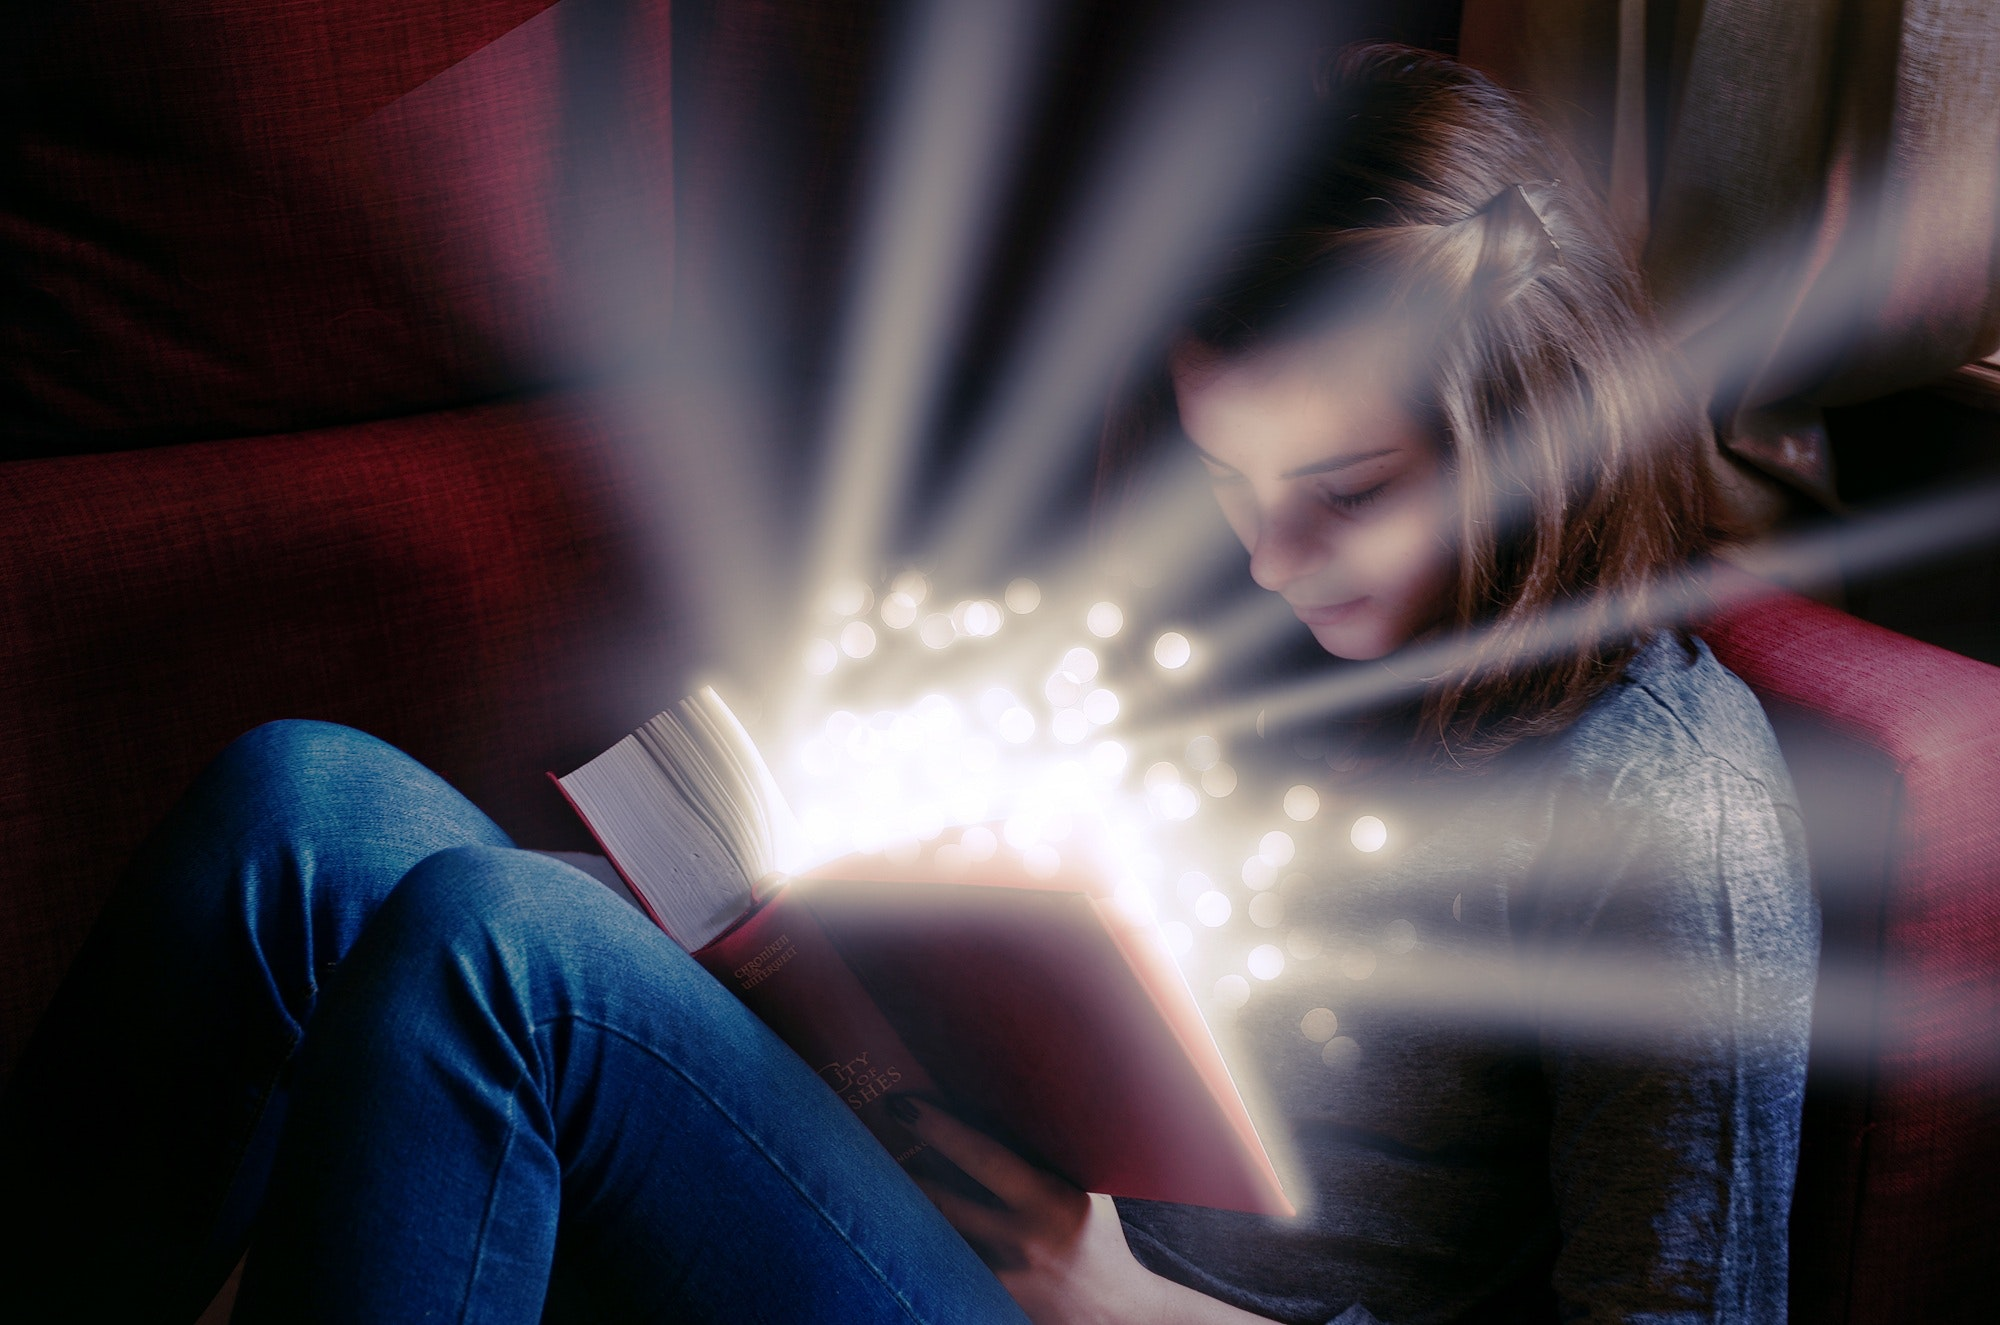
\includegraphics[width=10cm,keepaspectratio]{story_time}
  \end{center}
\end{frame}

\setbeamertemplate{footline}{}

\begin{frame}[t]
  \begin{center}
    \begingroup
    \fontsize{20pt}{20pt}\selectfont
    A Day in the Life \\
    \endgroup
    \bigskip
    \includegraphics[width=9cm,keepaspectratio]{server_room} \\
    \bigskip
    \inserttitle \\
  \end{center}
\end{frame}

\setbeamertemplate{footline}[myfootline]

\begin{frame}
  \frametitle{Morning}
  \framesubtitle{A Day in the Life 0 - Morning}
  \begin{columns}[onlytextwidth]
    \begin{column}{.30\textwidth}
      \begin{figure}
        
\includegraphics[width=5.5cm,keepaspectratio]{morning}
        \caption{Morning}
      \end{figure}
    \end{column}
    \hfill
    \begin{column}{.60\textwidth}
        \begin{tcolorbox}[title=social\_media.log,colback=gray]
          Coffee, Emails, Checking Threat Feeds and Cyber Securtiy News, Malware Analysis, Reverse Engineering, IDS Rule Development
        \end{tcolorbox}
    \end{column}
  \end{columns}
\end{frame}

\begin{frame}
  \frametitle{Analysis from Threat Intelligence}
  \framesubtitle{A Day in the Life 1 - Analysis from Threat Intelligence}
  \begin{center}
    \begin{figure}
    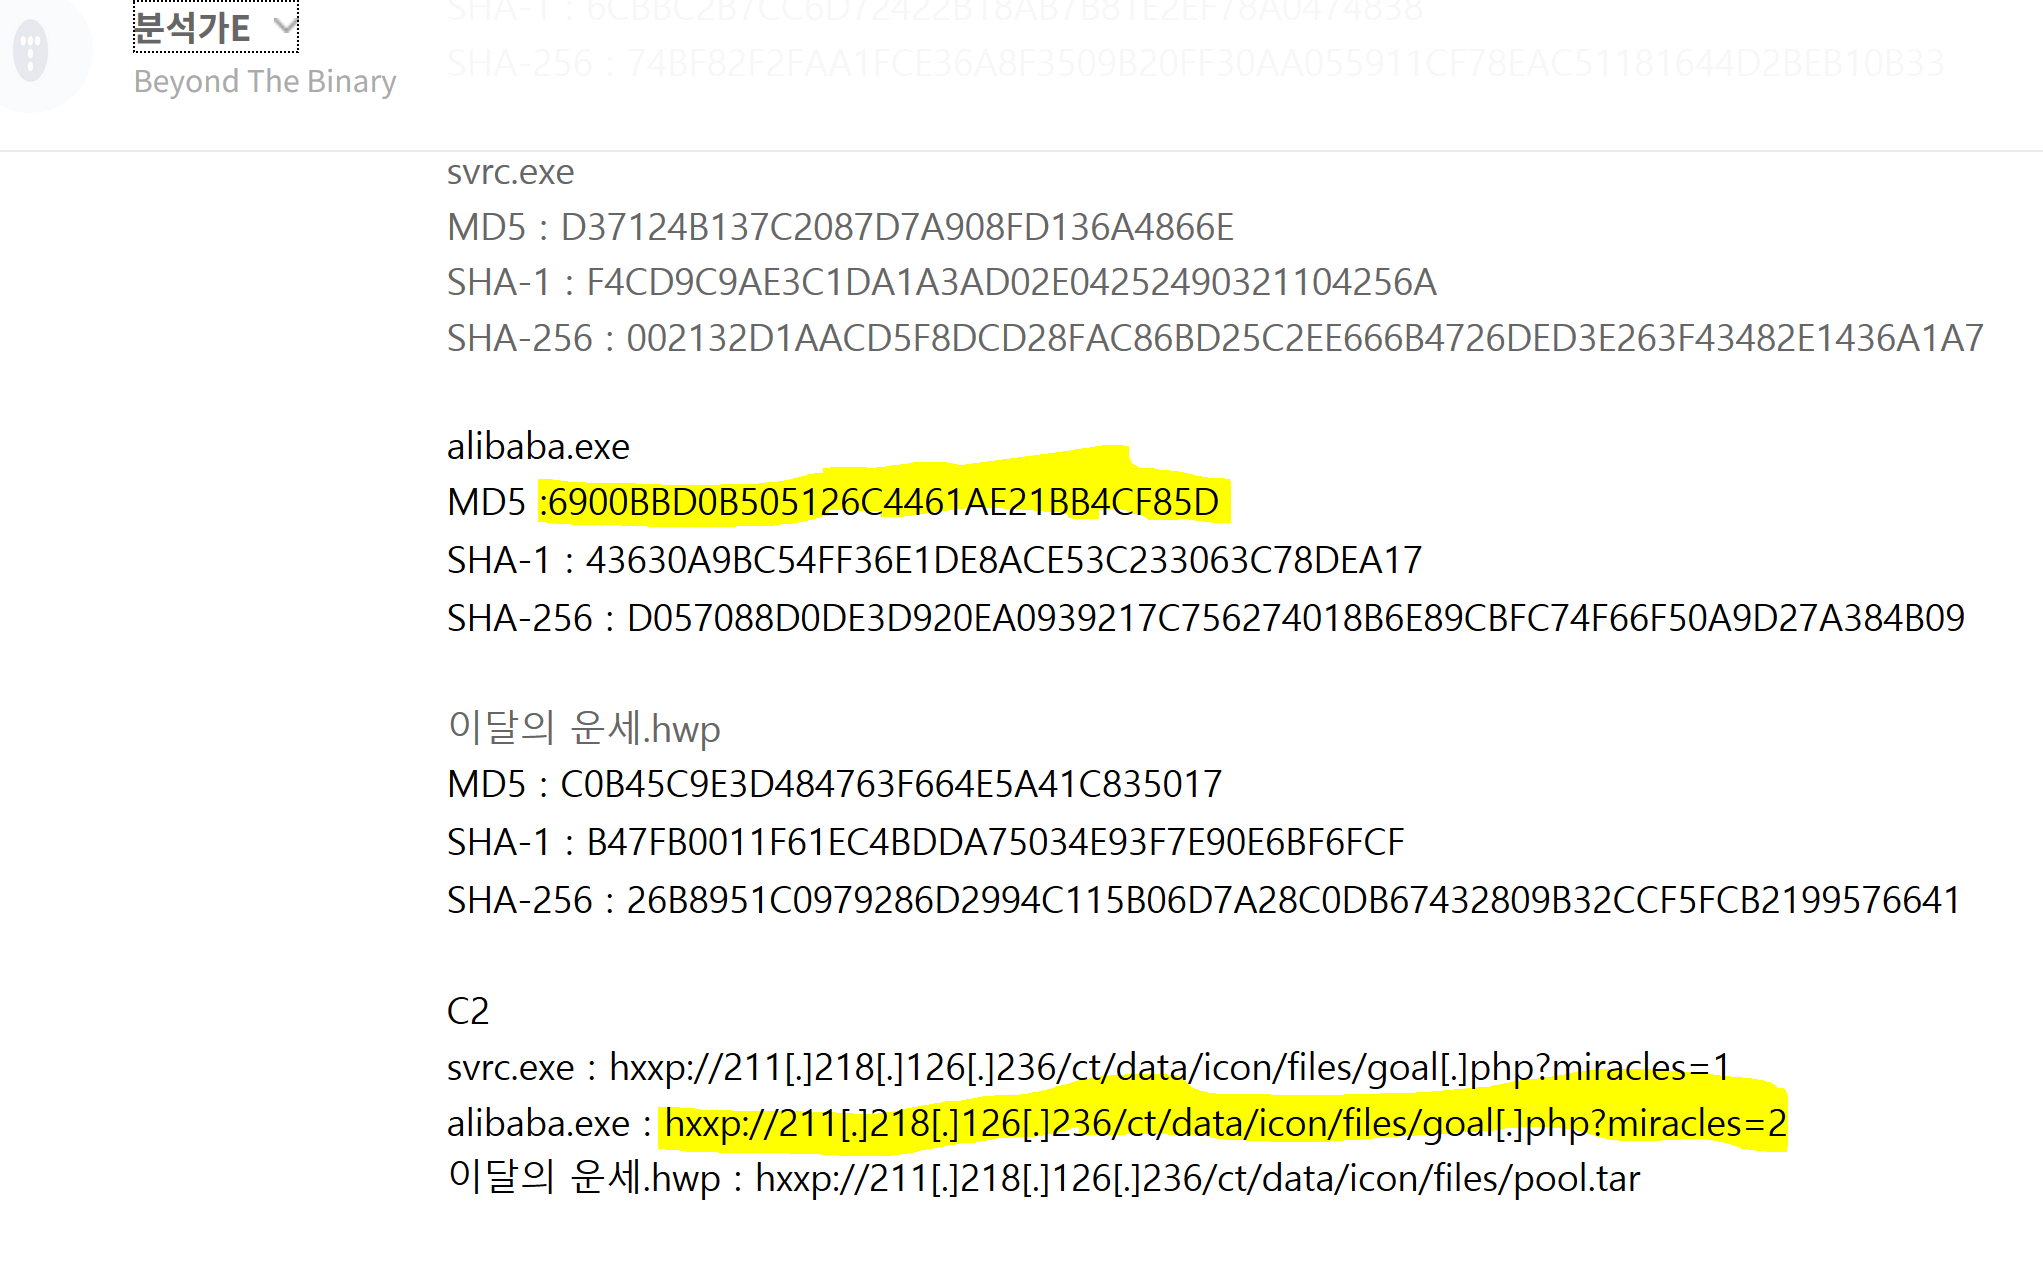
\includegraphics[width=10cm,keepaspectratio]{alibaba_article_0}
    \caption{Alibaba - Article}
    \end{figure}
  \end{center}
\end{frame}

\begin{frame}
  \frametitle{Analysis from Threat Intelligence}
  \framesubtitle{A Day in the Life 2 - Analysis from Threat Intelligence}
  \begin{center}
    \begin{figure}
    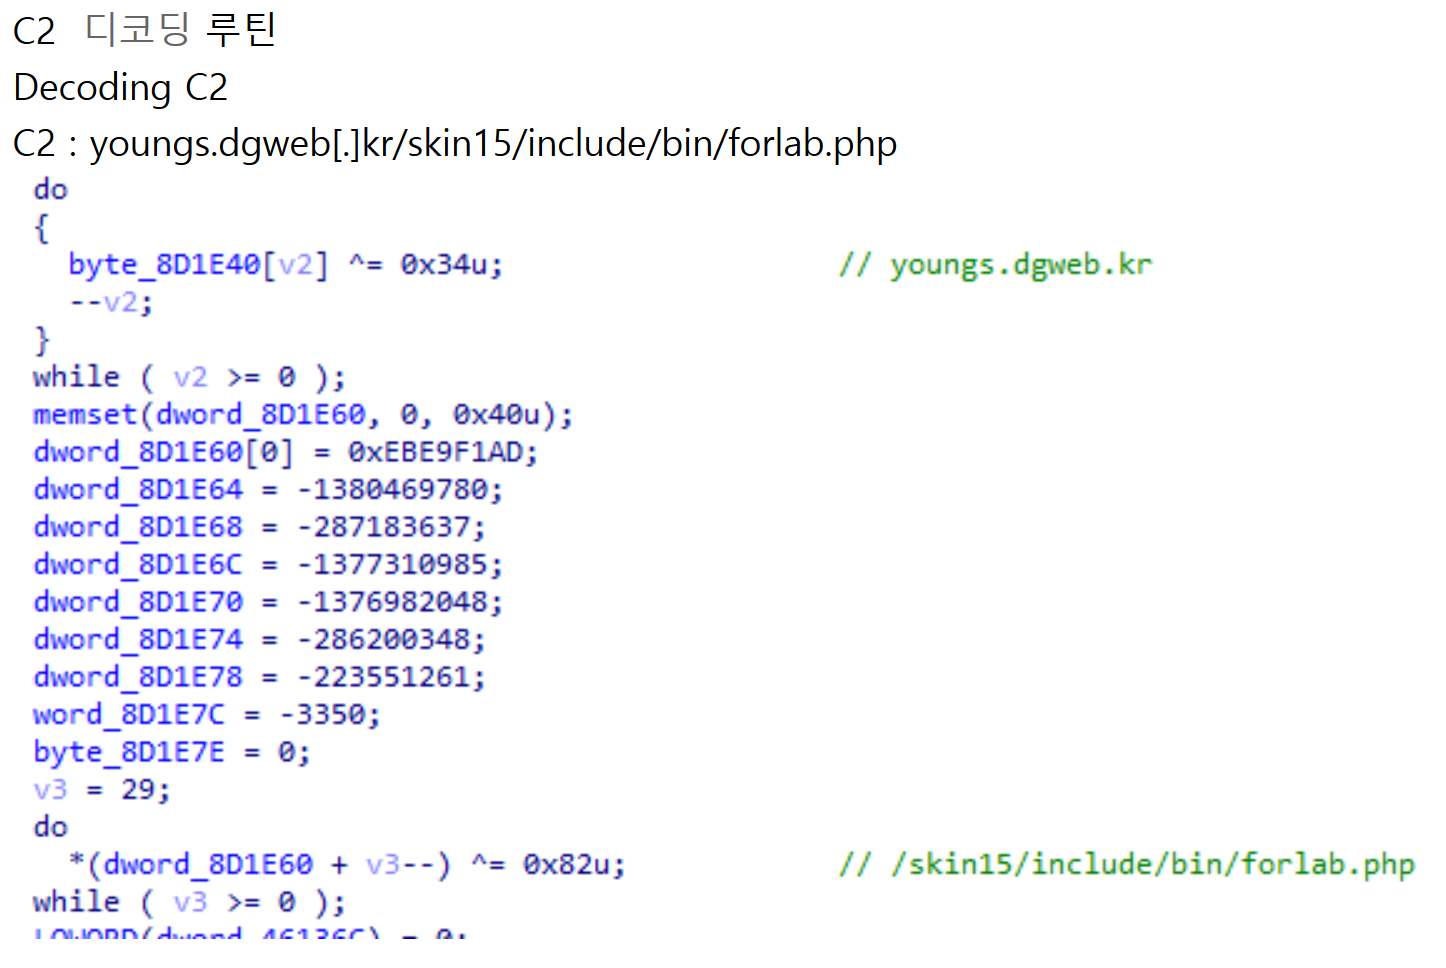
\includegraphics[width=8cm,keepaspectratio]{alibaba_article_1}
    \caption{Alibaba - Decoding the C2}
    \end{figure}
  \end{center}
\end{frame}

\begin{frame}
  \frametitle{Analysis from Threat Intelligence}
  \framesubtitle{A Day in the Life 3 - Analysis from Threat Intelligence}
  \begin{center}
    \begin{figure}
    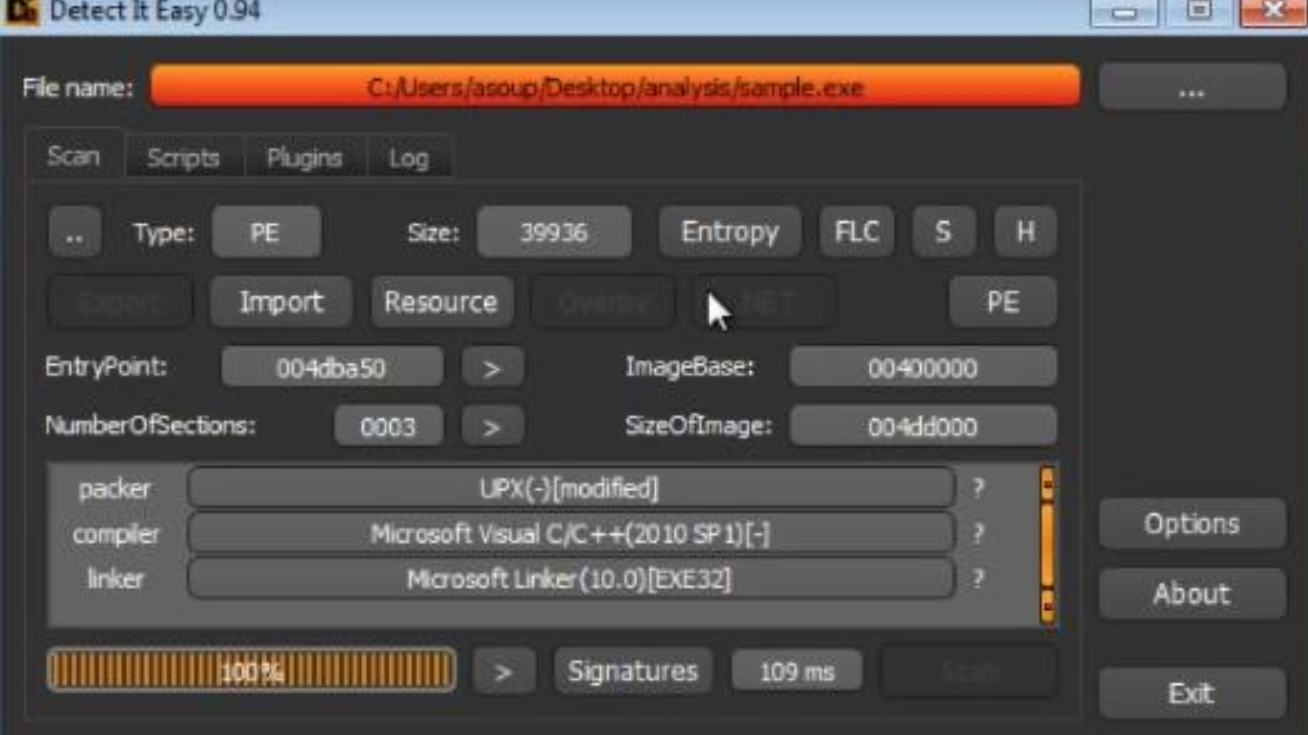
\includegraphics[width=8cm,keepaspectratio]{alibaba_die_main}
    \caption{Alibaba - UPX Packer}
    \end{figure}
  \end{center}
\end{frame}

\begin{frame}
  \frametitle{Analysis from Threat Intelligence}
  \framesubtitle{A Day in the Life 4 - Analysis from Threat Intelligence}
  \begin{center}
    \begin{figure}
      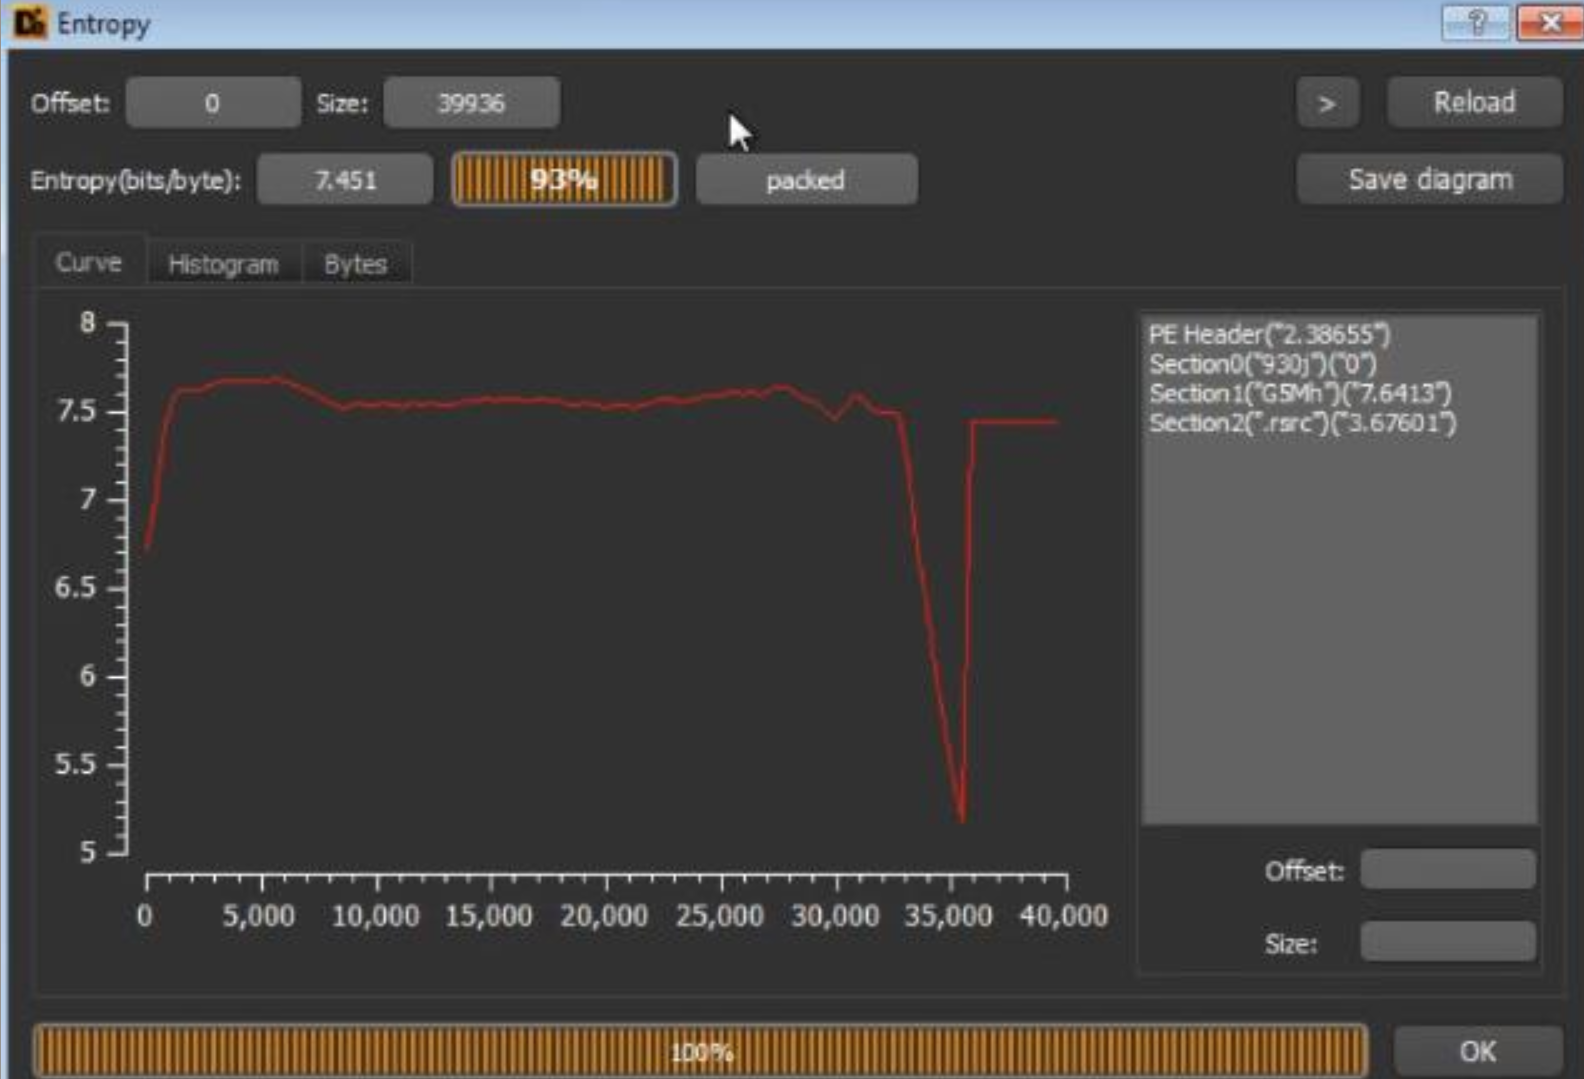
\includegraphics[width=8cm,keepaspectratio]{alibaba_die_entropy}
      \caption{Alibaba - High Entropy}
    \end{figure}
  \end{center}
\end{frame}

\begin{frame}
  \frametitle{Analysis from Threat Intelligence}
  \framesubtitle{A Day in the Life 5 - Analysis from Threat Intelligence}
  \begin{center}
    \begin{figure}
      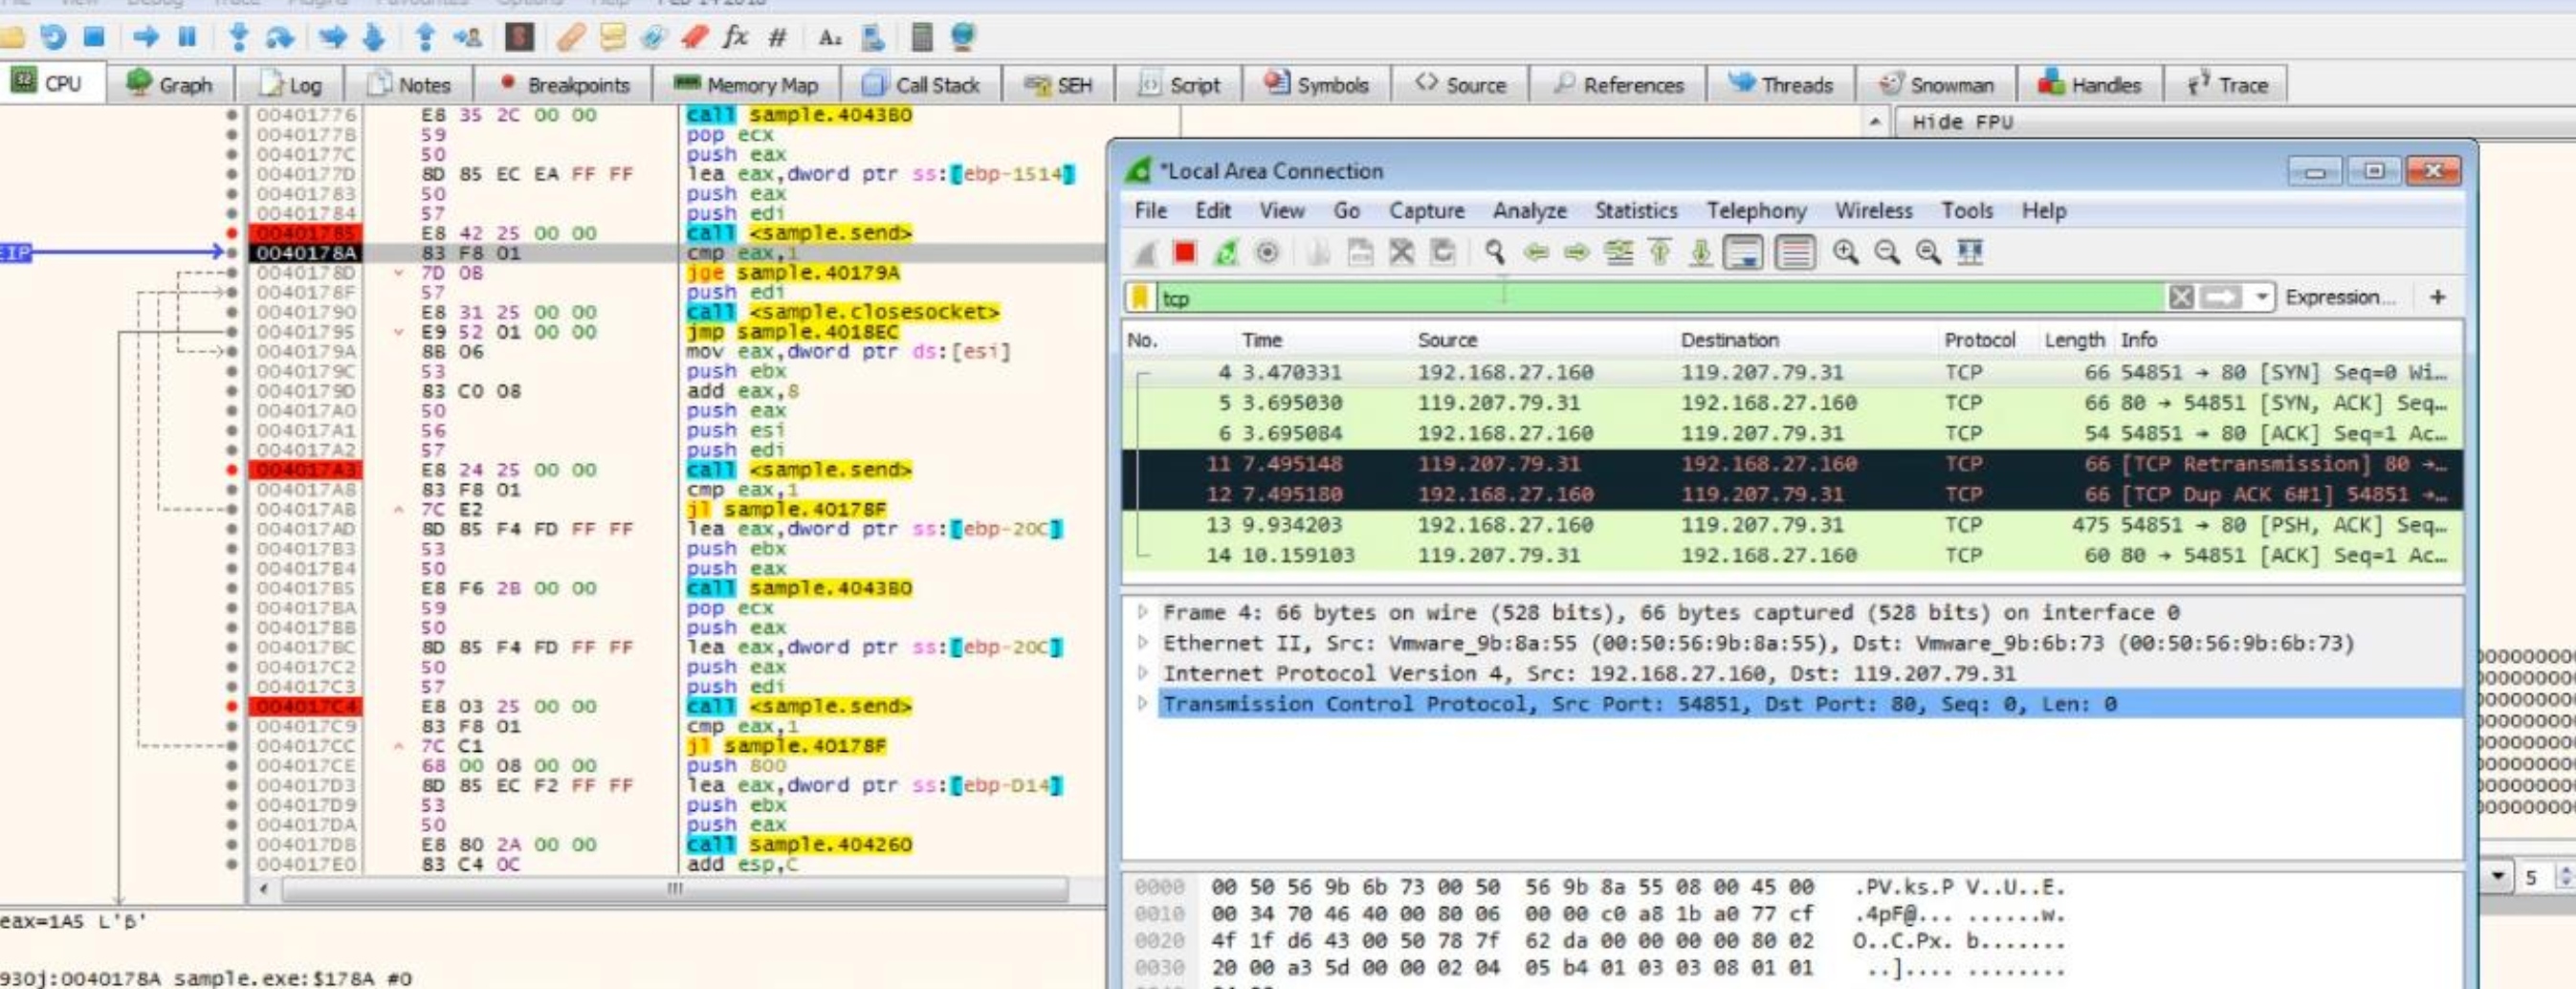
\includegraphics[width=14cm,keepaspectratio]{alibaba_cnc}
      \caption{Alibaba - Capturing the CnC}
    \end{figure}
  \end{center}
\end{frame}

\begin{frame}
  \frametitle{Analysis from Threat Intelligence}
  \framesubtitle{A Day in the Life 6 - Analysis from Threat Intelligence}
  \begin{center}
    \begin{figure}
      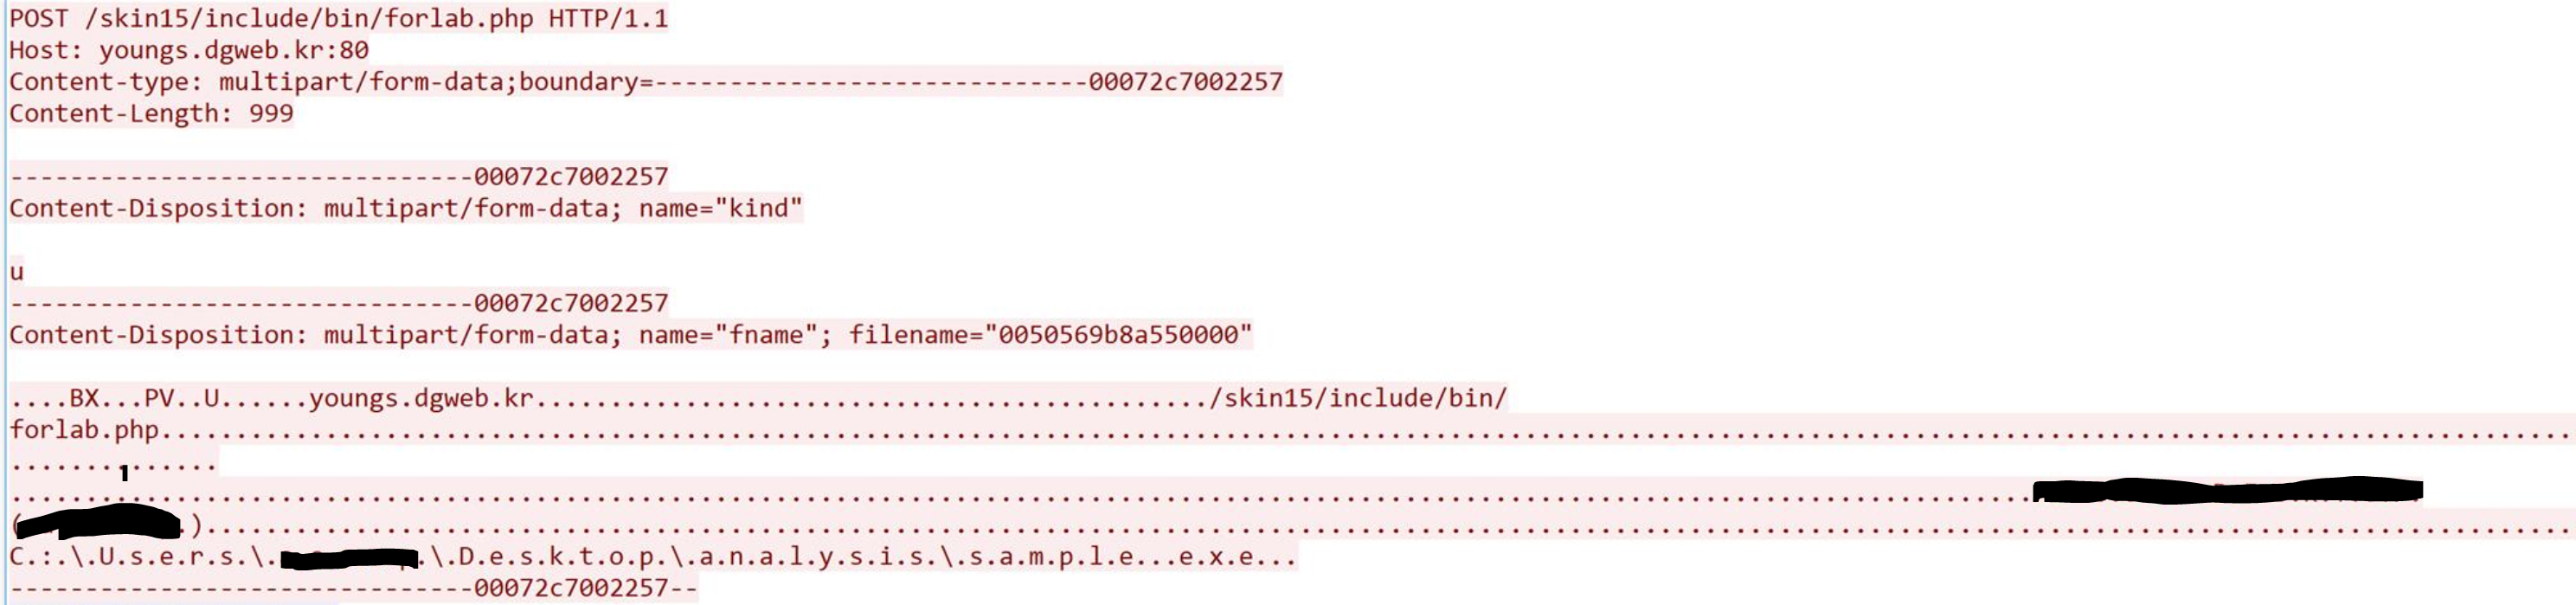
\includegraphics[width=14cm,keepaspectratio]{alibaba_http}
      \caption{Alibaba - Analysis of the CnC Packet}
    \end{figure}
  \end{center}
\end{frame}

\begin{frame}
  \frametitle{Analysis from Threat Intelligence}
  \framesubtitle{A Day in the Life 7 - Analysis from Threat Intelligence}
  \begin{center}
    \begin{figure}
      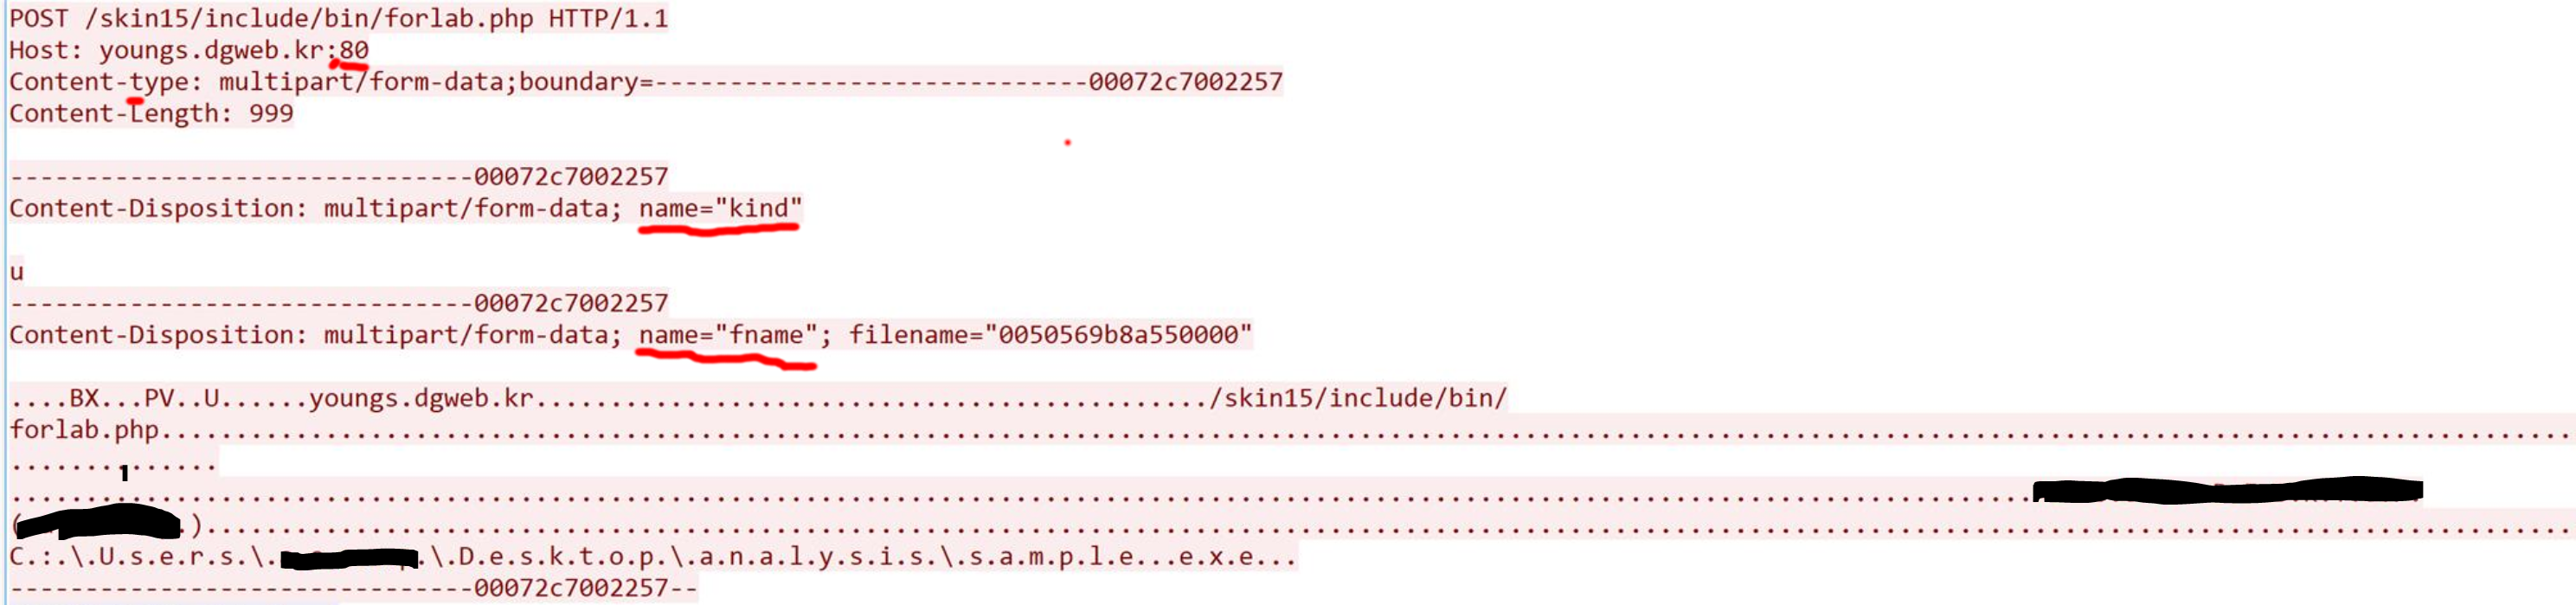
\includegraphics[width=14cm,keepaspectratio]{alibaba_http_highlight}
      \caption{Alibaba - Analysis of the CnC Packet}
    \end{figure}
  \end{center}
\end{frame}

\begin{frame}
  \frametitle{Analysis from Threat Intelligence}
  \framesubtitle{A Day in the Life 8 - Analysis from Threat Intelligence}
  \begin{center}
    \begin{figure}
      
\includegraphics[width=9cm,keepaspectratio]{fancybear_logo}
      \caption{Fancy Bear - APT Group}
    \end{figure}
  \end{center}
\end{frame}

\begin{frame}
  \frametitle{Analysis from Threat Intelligence}
  \framesubtitle{A Day in the Life 9 - Analysis from Threat Intelligence}
  \begin{center}
    \begin{figure}
      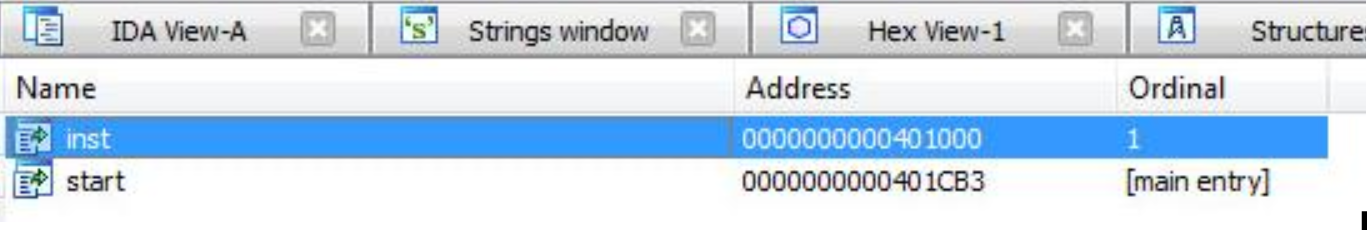
\includegraphics[width=14cm,keepaspectratio]{fancy_bear_analysis_0}
      \caption{Fancy Bear - DLL Export}
    \end{figure}
  \end{center}
\end{frame}

\begin{frame}
  \frametitle{Analysis from Threat Intelligence}
  \framesubtitle{A Day in the Life 10 - Analysis from Threat Intelligence}
  \begin{center}
    \begin{figure}
      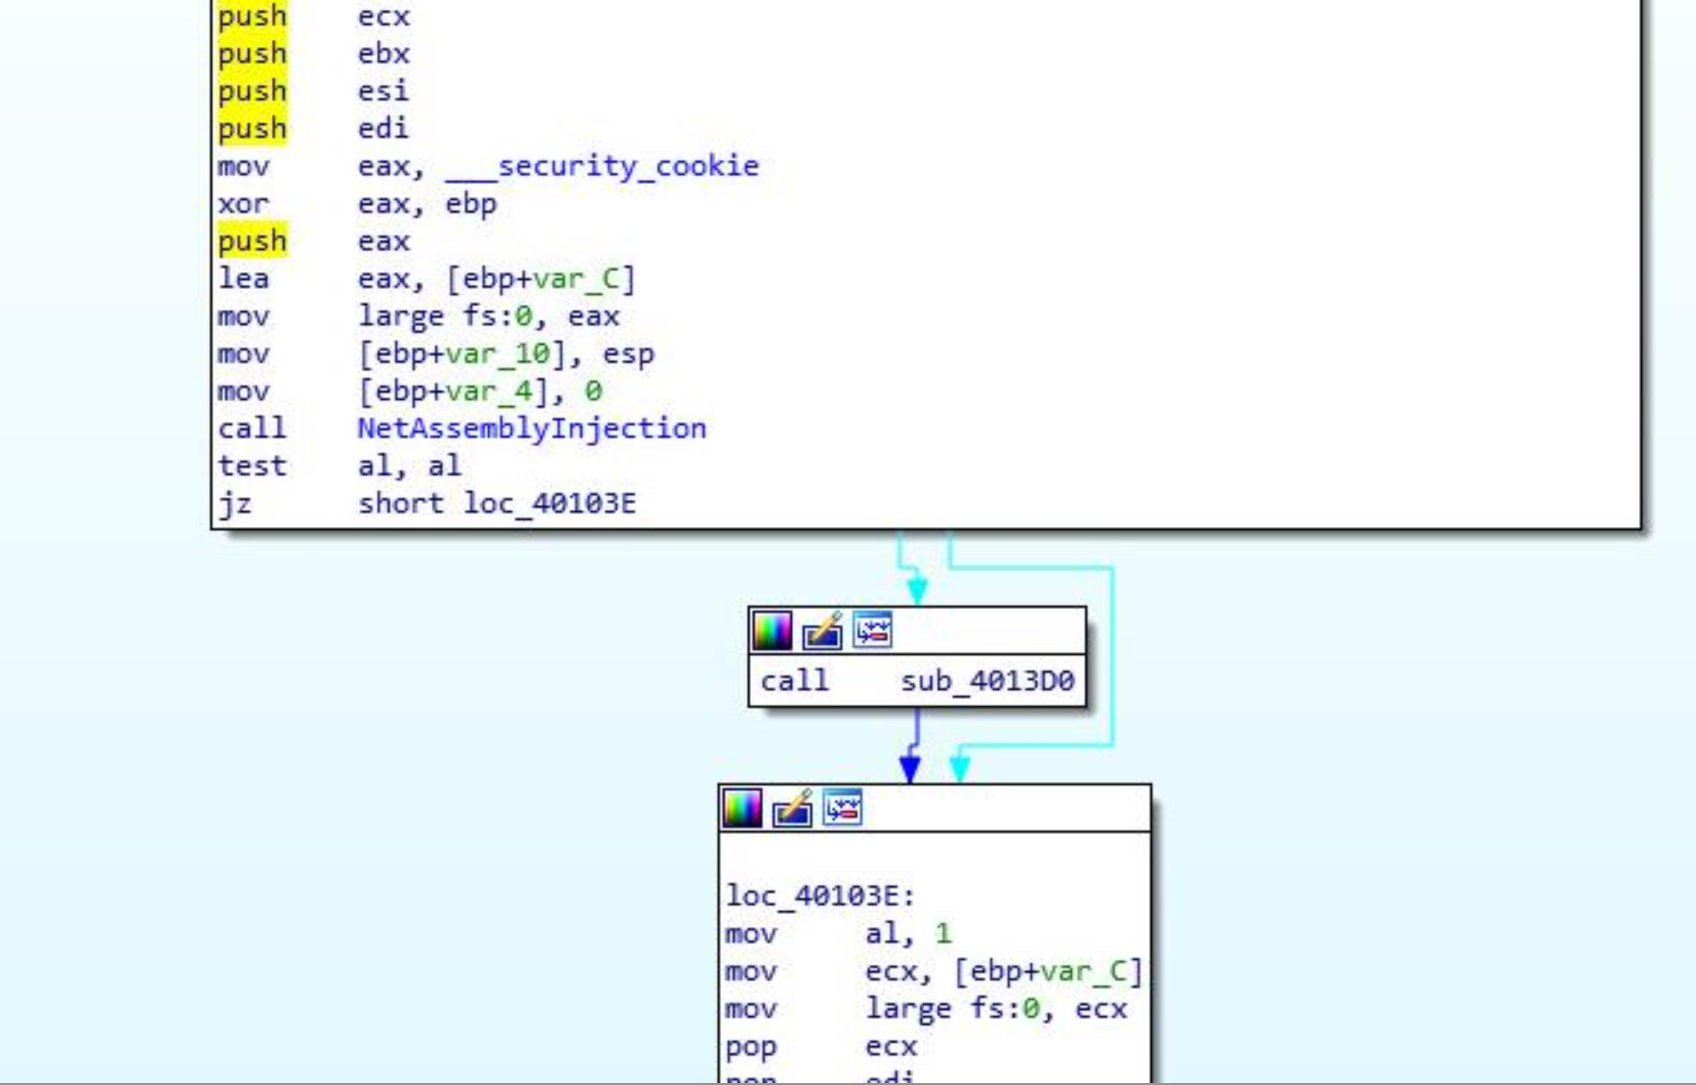
\includegraphics[width=8cm,keepaspectratio]{fancy_bear_analysis_1}
      \caption{Fancy Bear - .NET Assembly Injection}
    \end{figure}
  \end{center}
\end{frame}

\begin{frame}
  \frametitle{Analysis from Threat Intelligence}
  \framesubtitle{A Day in the Life 11 - Analysis from Threat Intelligence}
  \begin{center}
    \begin{figure}
      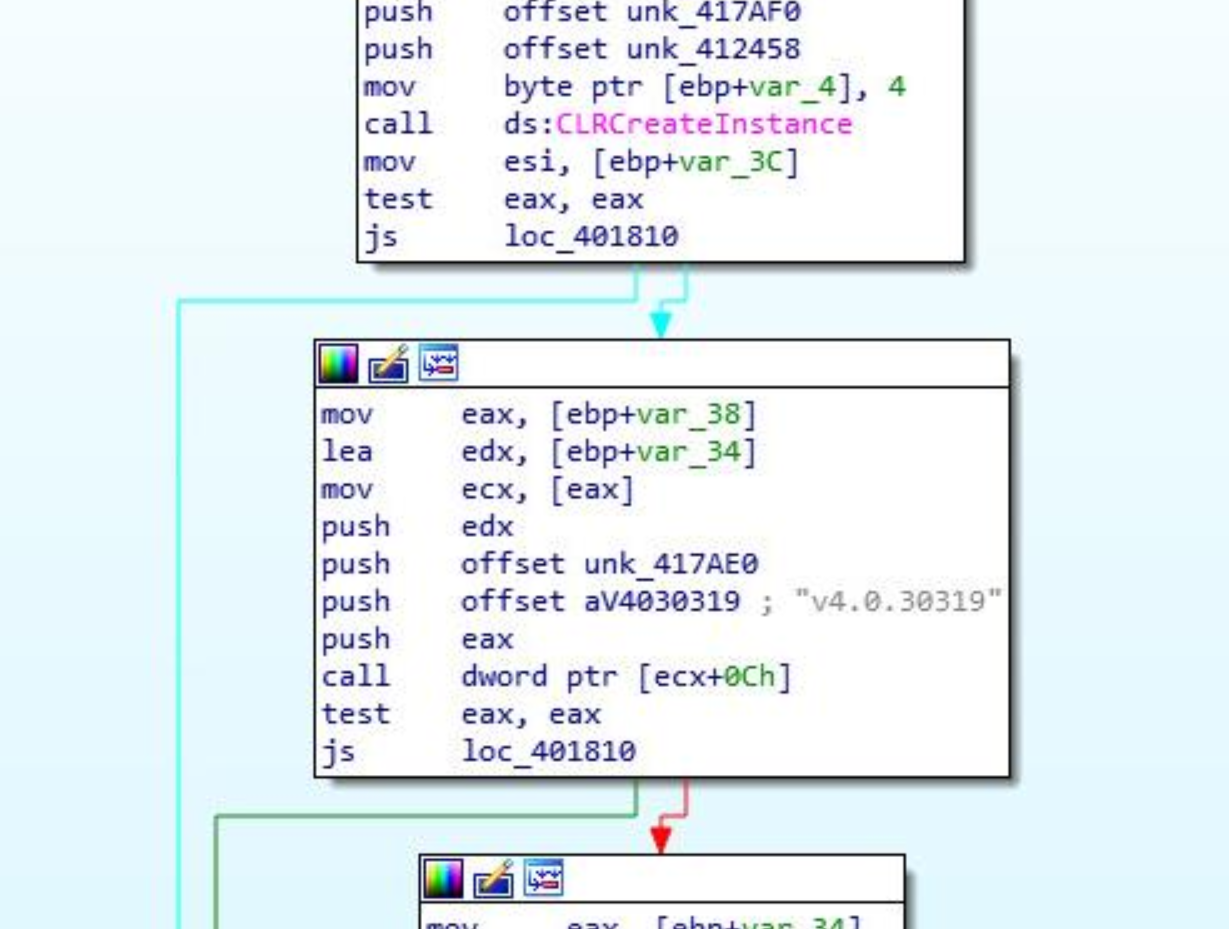
\includegraphics[width=8cm,keepaspectratio]{fancy_bear_analysis_2}
      \caption{Fancy Bear - Loading .NET Assembly Version}
    \end{figure}
  \end{center}
\end{frame}

\begin{frame}
  \frametitle{Analysis from Threat Intelligence}
  \framesubtitle{A Day in the Life 12 - Analysis from Threat Intelligence}
  \begin{center}
    \begin{figure}
      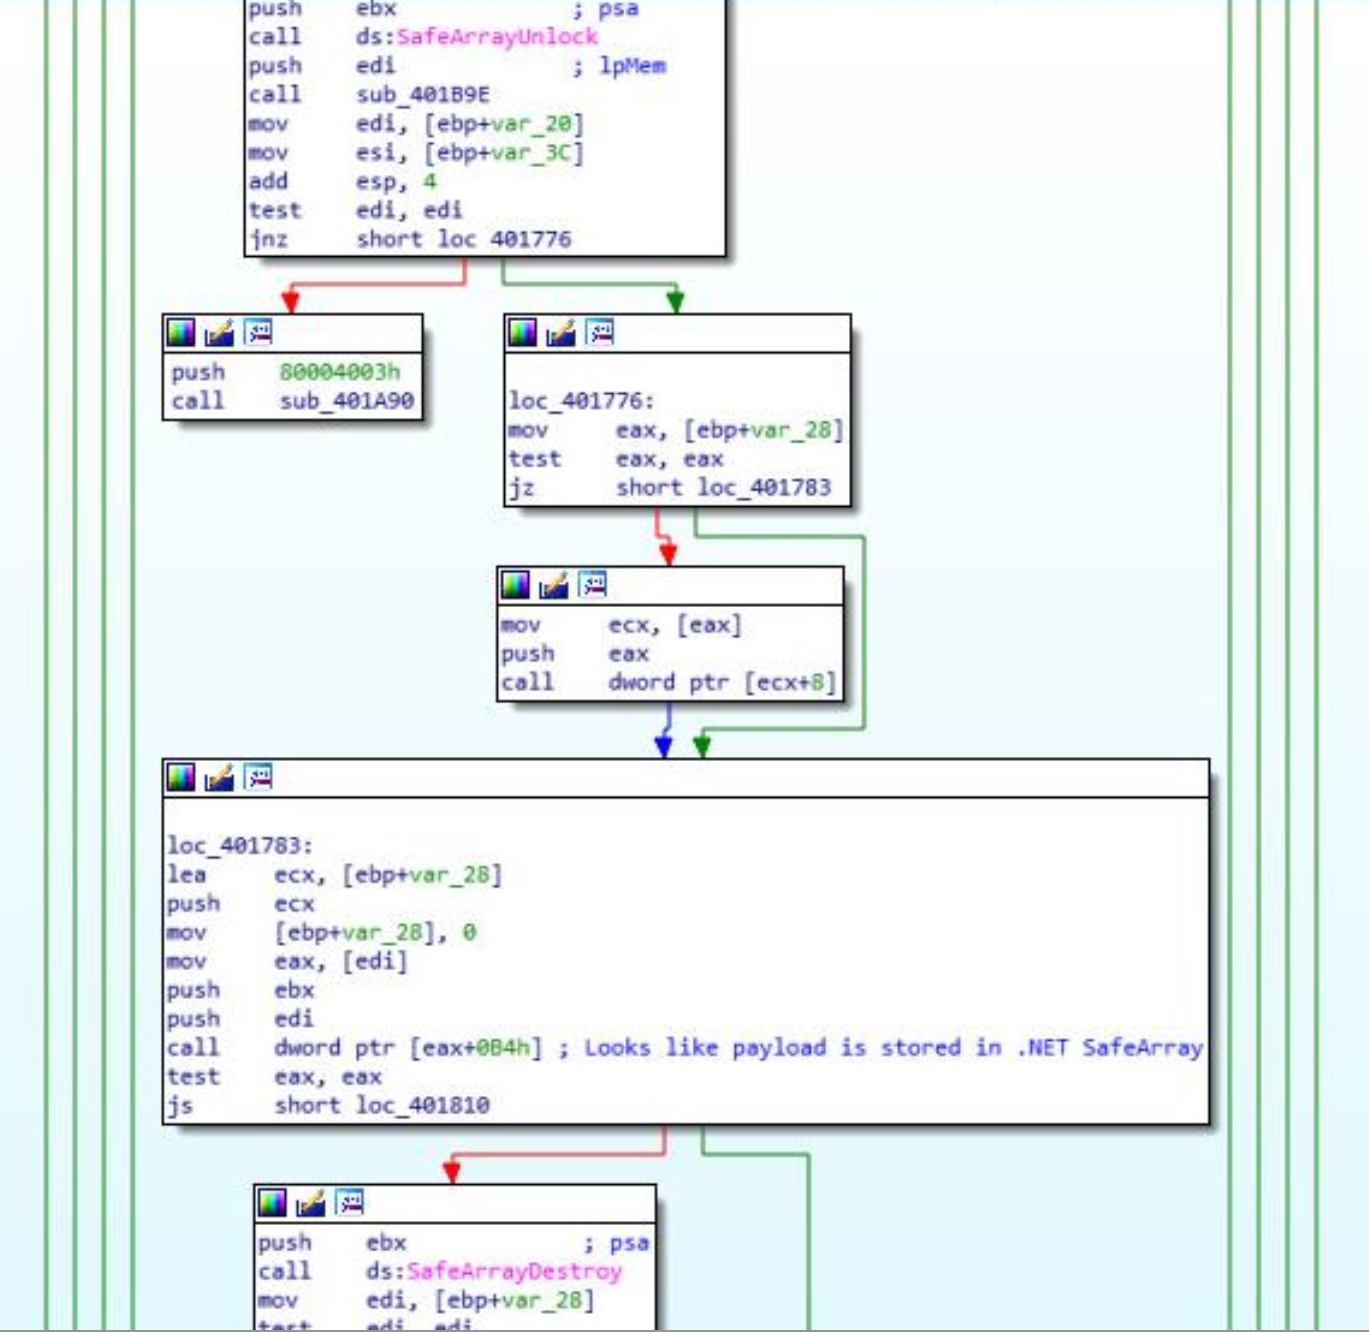
\includegraphics[width=6.5cm,keepaspectratio]{fancy_bear_analysis_3}
      \caption{Fancy Bear - Searching for the Payload}
    \end{figure}
  \end{center}
\end{frame}

\begin{frame}
  \frametitle{Analysis from Threat Intelligence}
  \framesubtitle{A Day in the Life 13 - Analysis from Threat Intelligence}
  \begin{center}
    \begin{figure}
      \includegraphics[width=13.5cm,keepaspectratio]{fancy_bear_analysis_4}
      \caption{Fancy Bear - Found the Payload}
    \end{figure}
  \end{center}
\end{frame}

\begin{frame}
  \frametitle{Analysis from Threat Intelligence}
  \framesubtitle{A Day in the Life 14 - Analysis from Threat Intelligence}
  \begin{center}
    \begin{figure}
      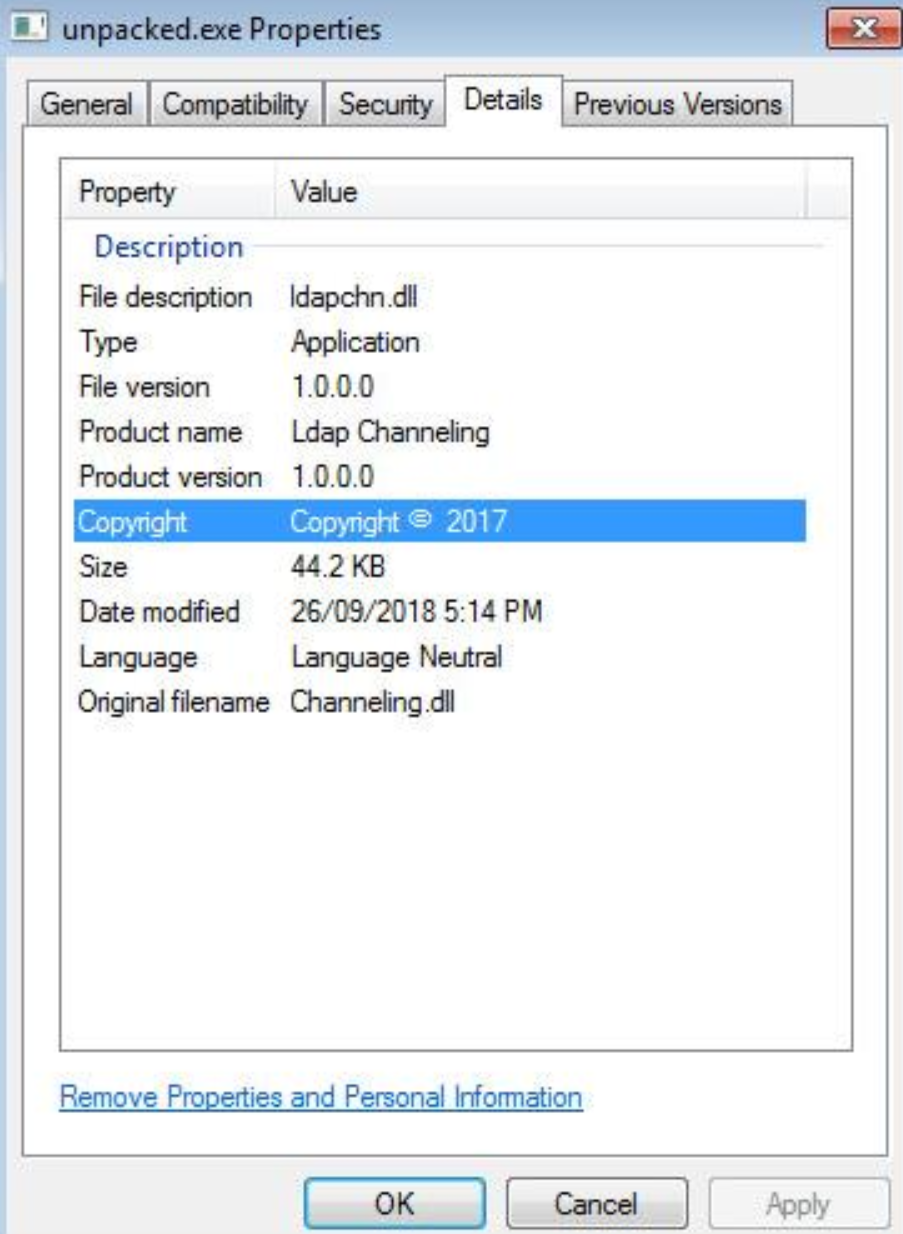
\includegraphics[width=4.5cm,keepaspectratio]{fancy_bear_analysis_5}
      \caption{Fancy Bear - Payload Properties}
    \end{figure}
  \end{center}
\end{frame}

\begin{frame}
  \frametitle{Analysis from Threat Intelligence}
  \framesubtitle{A Day in the Life 15 - Analysis from Threat Intelligence}
  \begin{center}
    \begin{figure}
      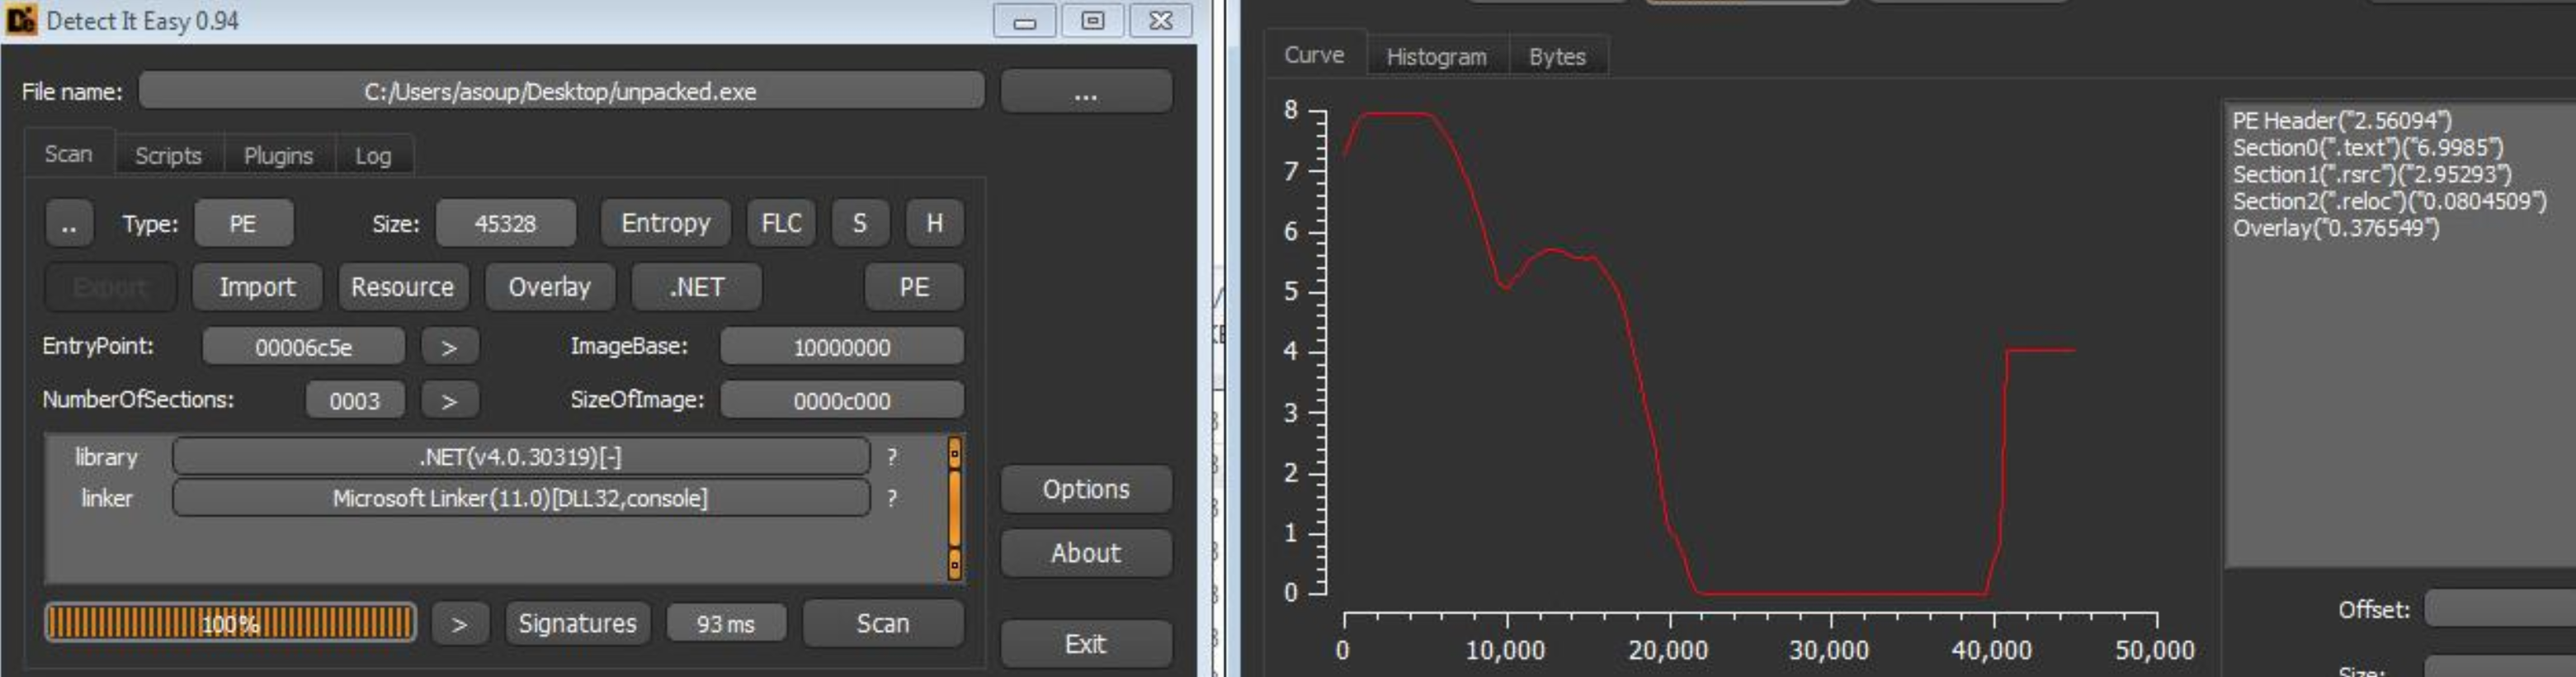
\includegraphics[width=14cm,keepaspectratio]{fancy_bear_analysis_6}
      \caption{Fancy Bear - Payload Entropy}
    \end{figure}
  \end{center}
\end{frame}

\begin{frame}
  \frametitle{Analysis from Threat Intelligence}
  \framesubtitle{A Day in the Life 16 - Analysis from Threat Intelligence}
  \begin{center}
    \begin{figure}
      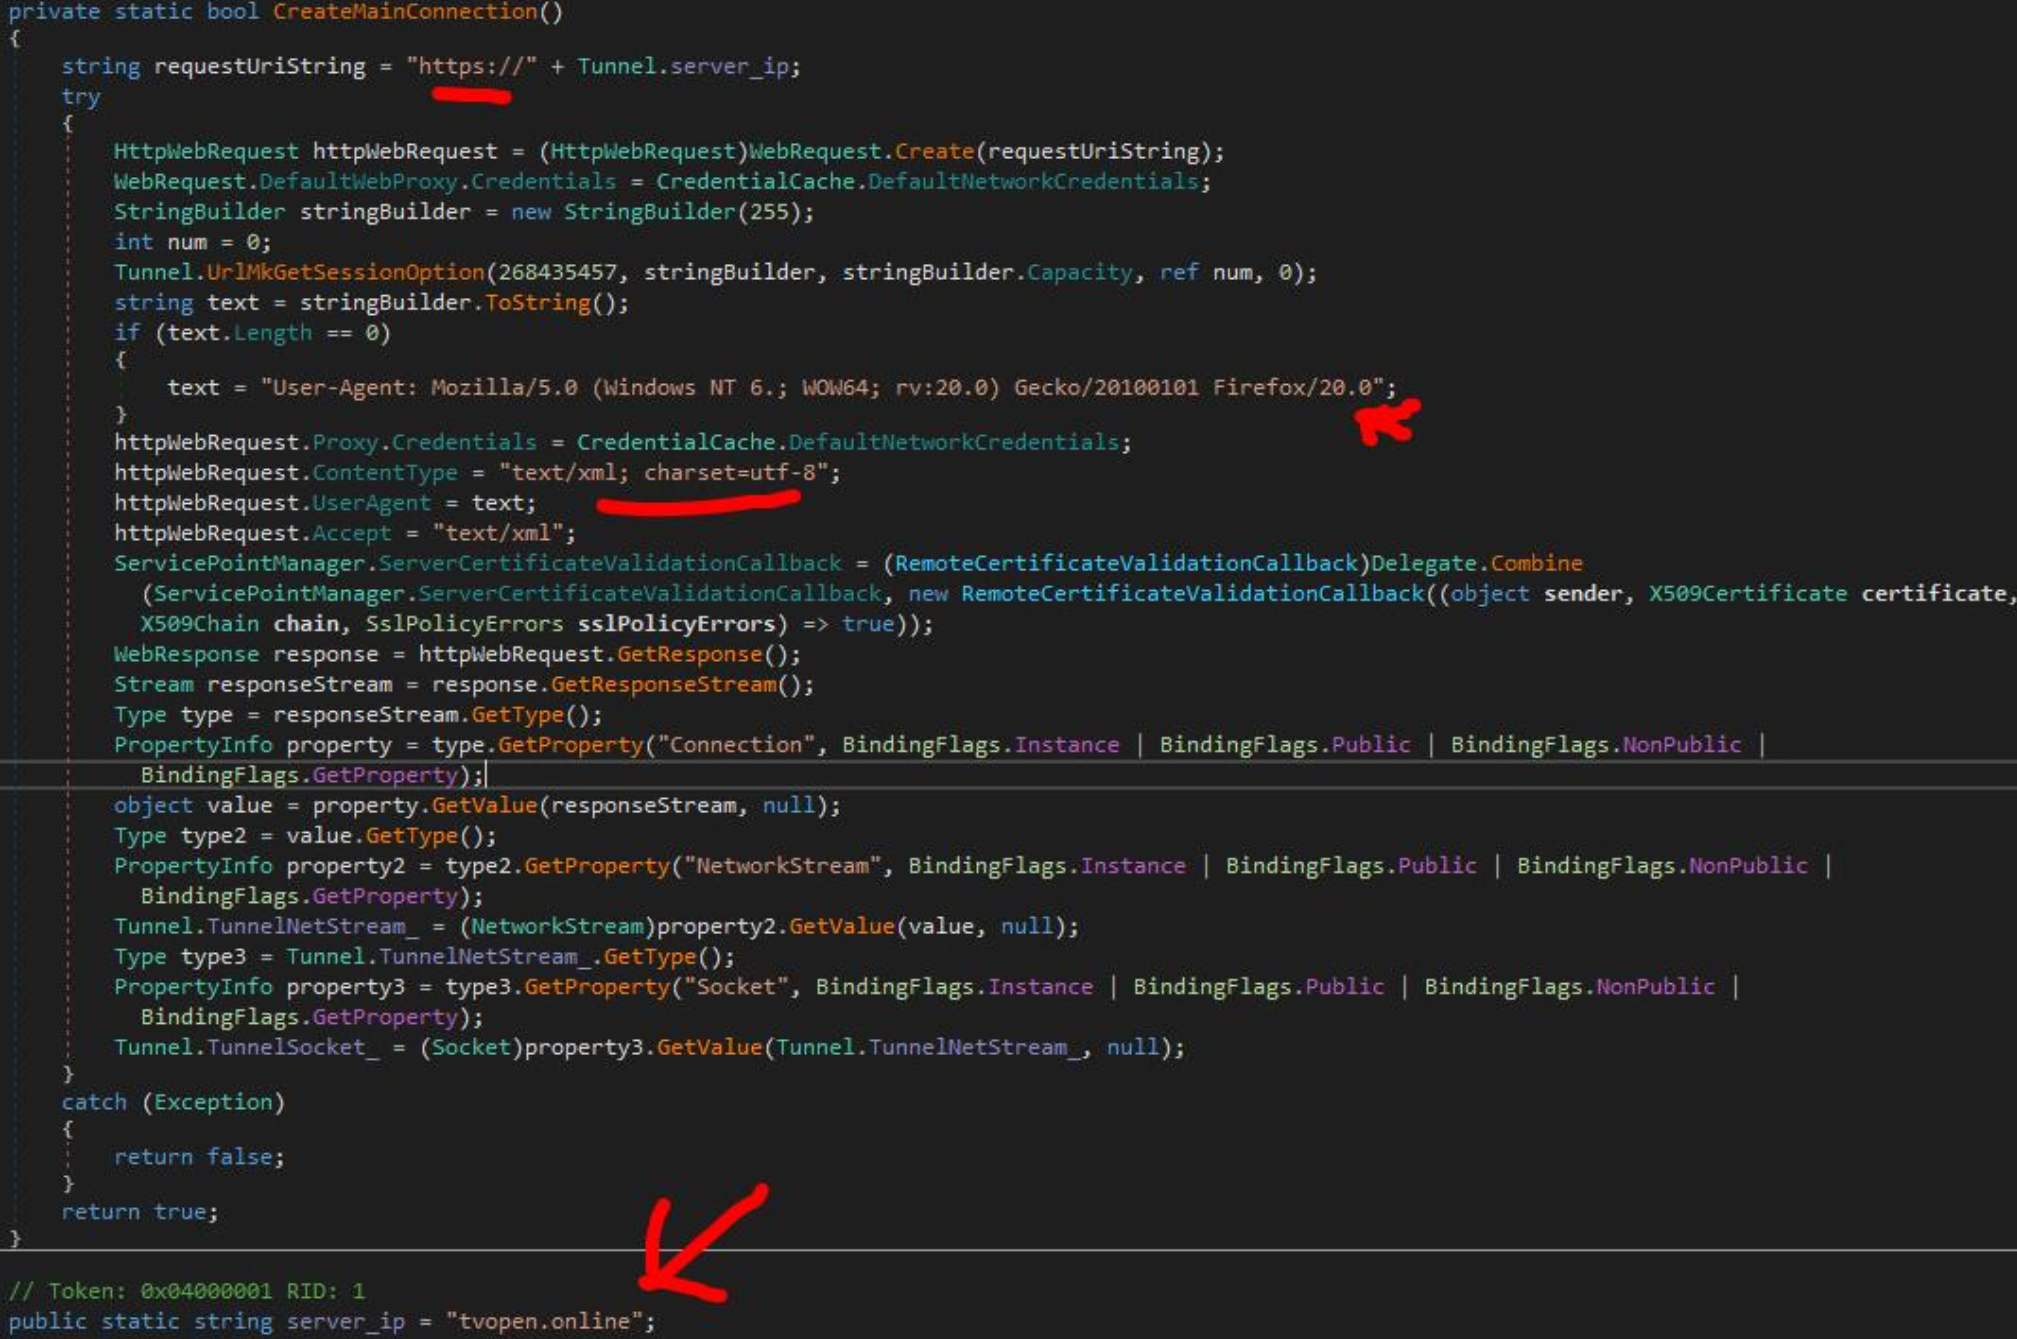
\includegraphics[width=9.5cm,keepaspectratio]{fancy_bear_analysis_7}
      \caption{Fancy Bear - Payload Decompiled .NET}
    \end{figure}
  \end{center}
\end{frame}

\begin{frame}
  \frametitle{Analysis from Threat Intelligence}
  \framesubtitle{A Day in the Life 17 - Analysis from Threat Intelligence}
  \begin{center}
    \begin{figure}
      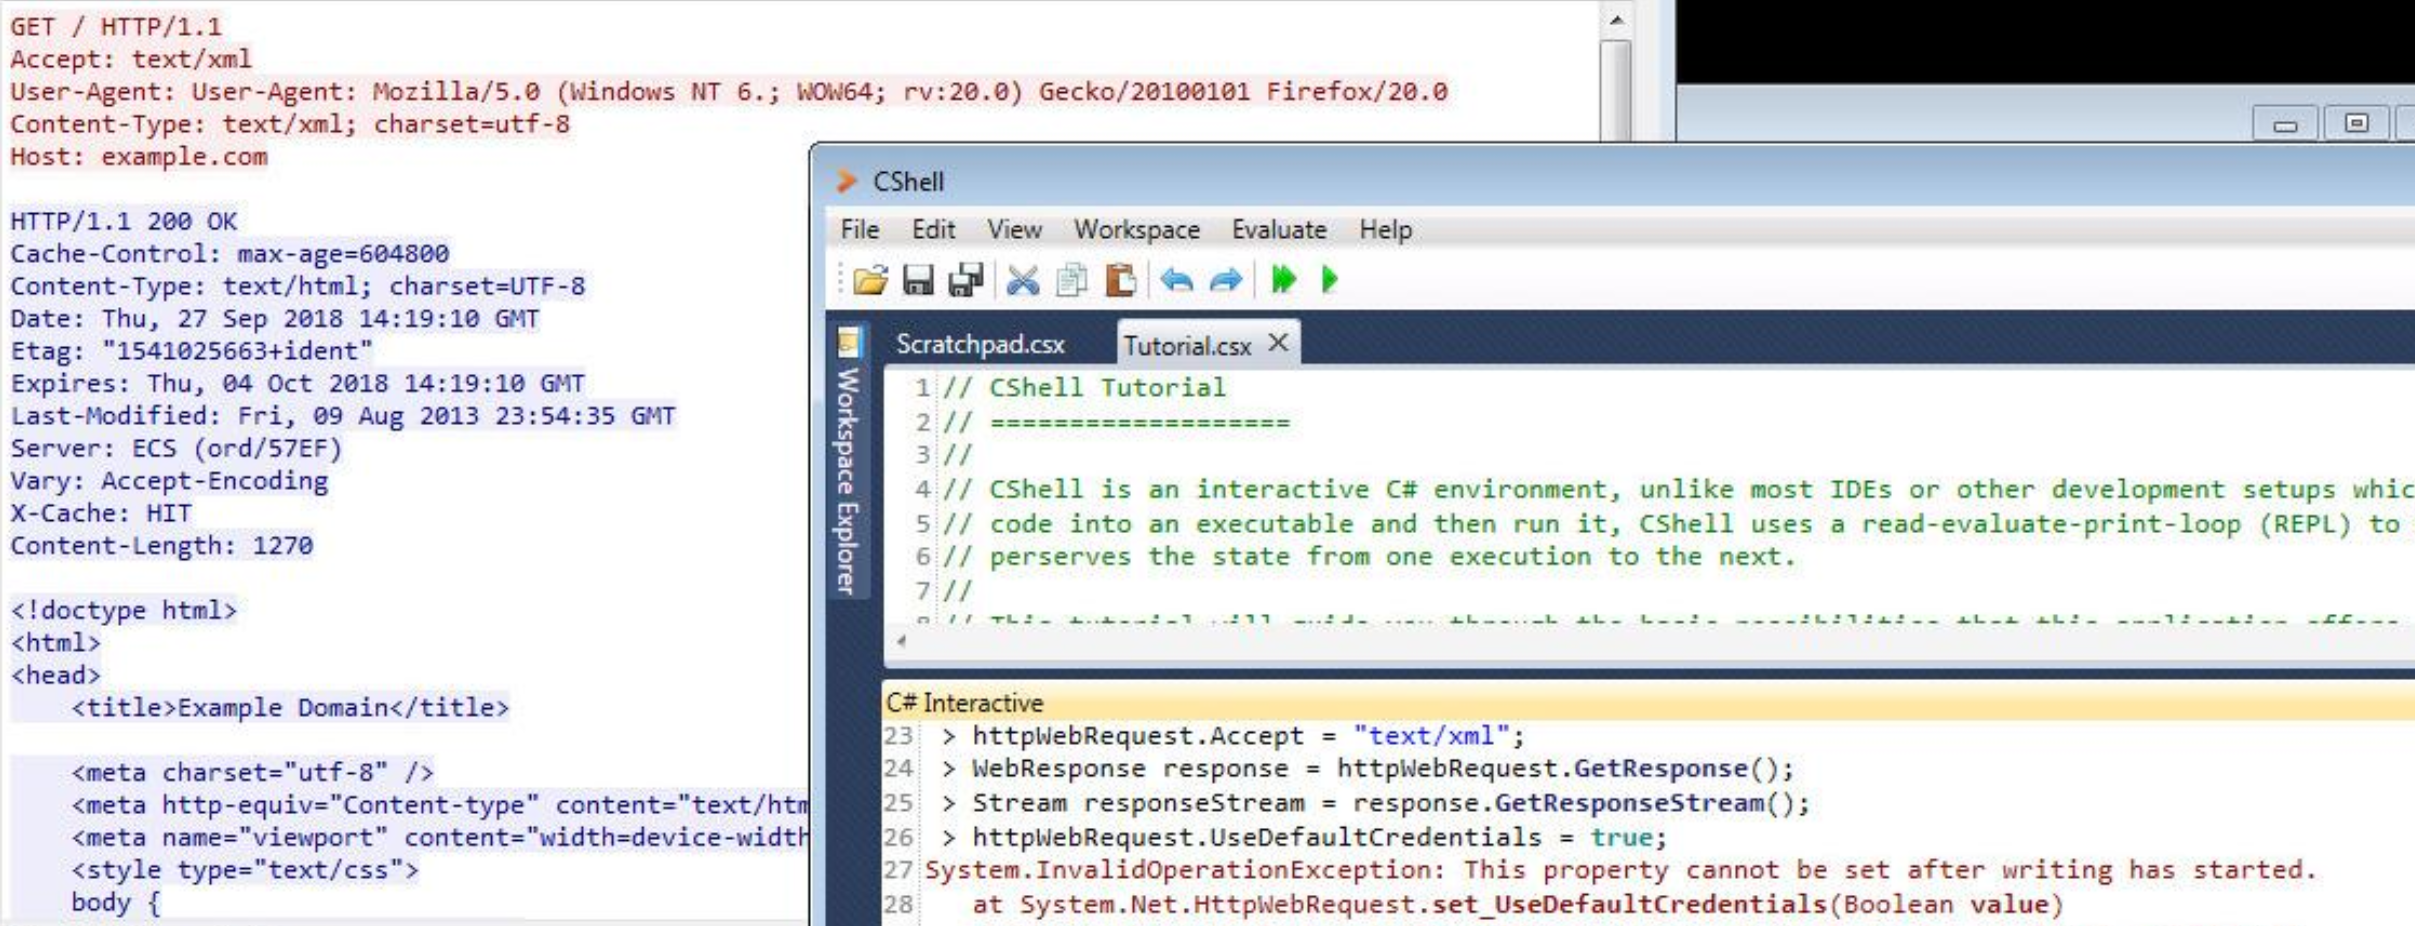
\includegraphics[width=14cm,keepaspectratio]{fancy_bear_analysis_8}
      \caption{Fancy Bear - Recreating the CnC Beacon}
    \end{figure}
  \end{center}
\end{frame}

\begin{frame}
  \frametitle{Analysis from Threat Intelligence}
  \framesubtitle{A Day in the Life 18 - Analysis from Threat Intelligence}
  \begin{center}
    \begin{figure}
      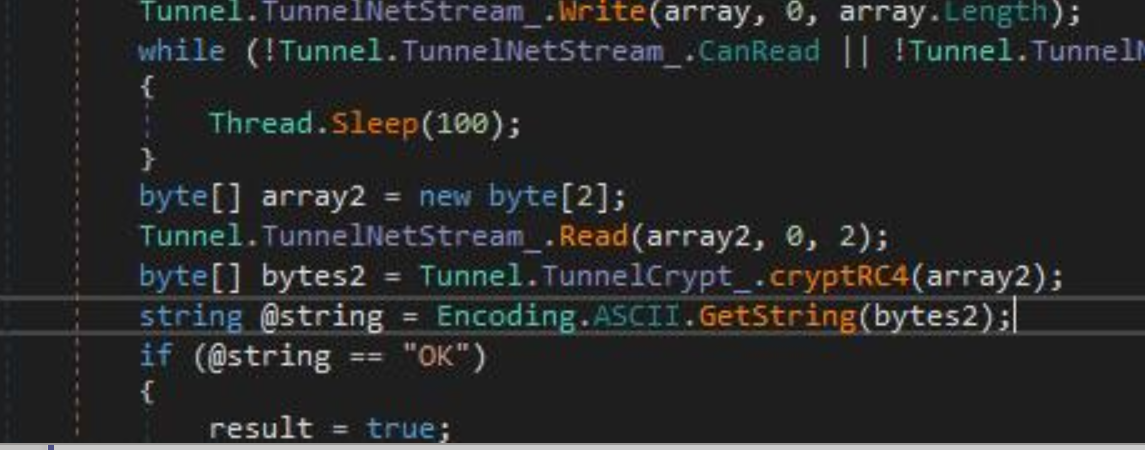
\includegraphics[width=14cm,keepaspectratio]{fancy_bear_analysis_9}
      \caption{Fancy Bear - APT for Sure}
    \end{figure}
  \end{center}
\end{frame}

\begin{frame}
  \frametitle{Analysis from Threat Intelligence}
  \framesubtitle{A Day in the Life 19 - Analysis from Threat Intelligence}
  \begin{center}
    \begin{figure}
      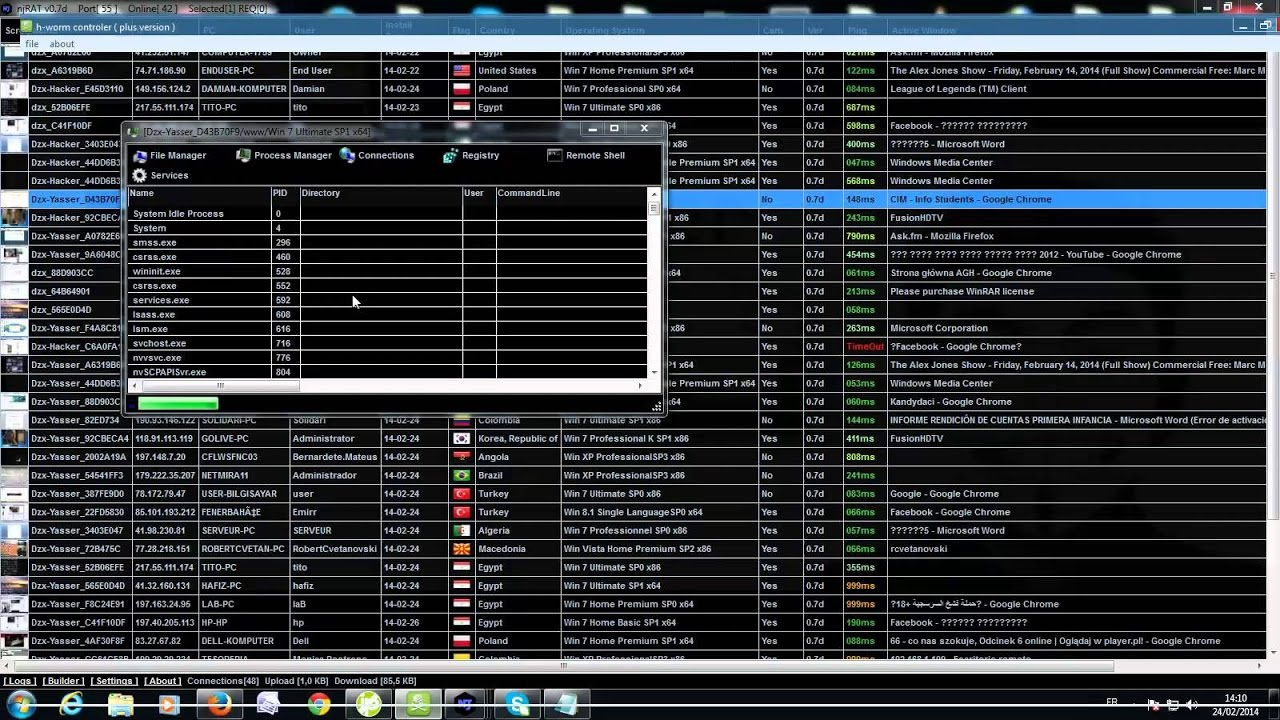
\includegraphics[width=10cm,keepaspectratio]{njrat}
      \caption{NJRat - Interface}
    \end{figure}
  \end{center}
\end{frame}

\begin{frame}
  \frametitle{Analysis from Threat Intelligence}
  \framesubtitle{A Day in the Life 20 - Analysis from Threat Intelligence}
  \begin{center}
    \begin{figure}
      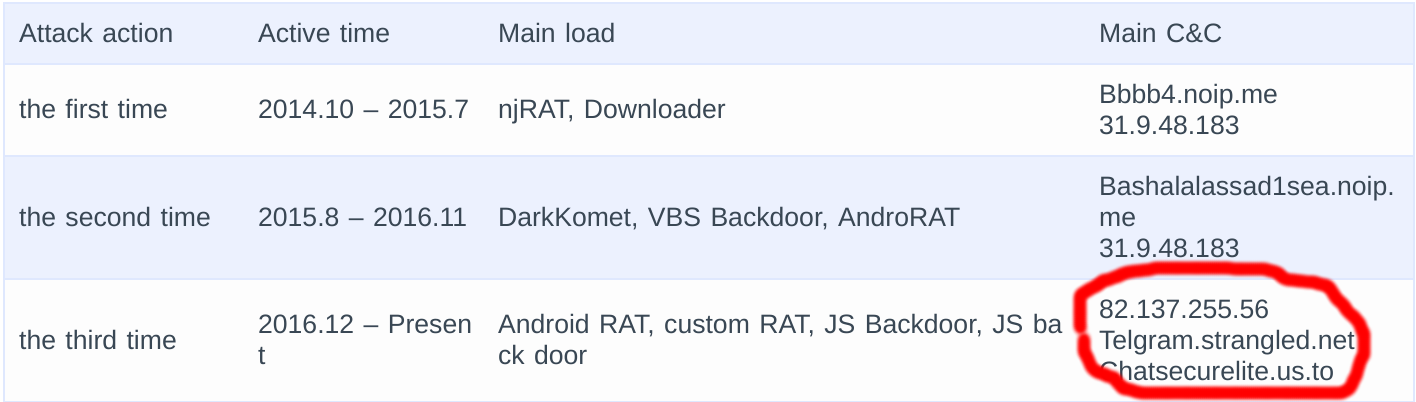
\includegraphics[width=14cm,keepaspectratio]{njrat_article}
      \caption{NJRat - Article}
    \end{figure}
  \end{center}
\end{frame}

\begin{frame}
  \frametitle{Analysis from Threat Intelligence}
  \framesubtitle{A Day in the Life 21 - Analysis from Threat Intelligence}
  \begin{center}
    \begin{figure}
      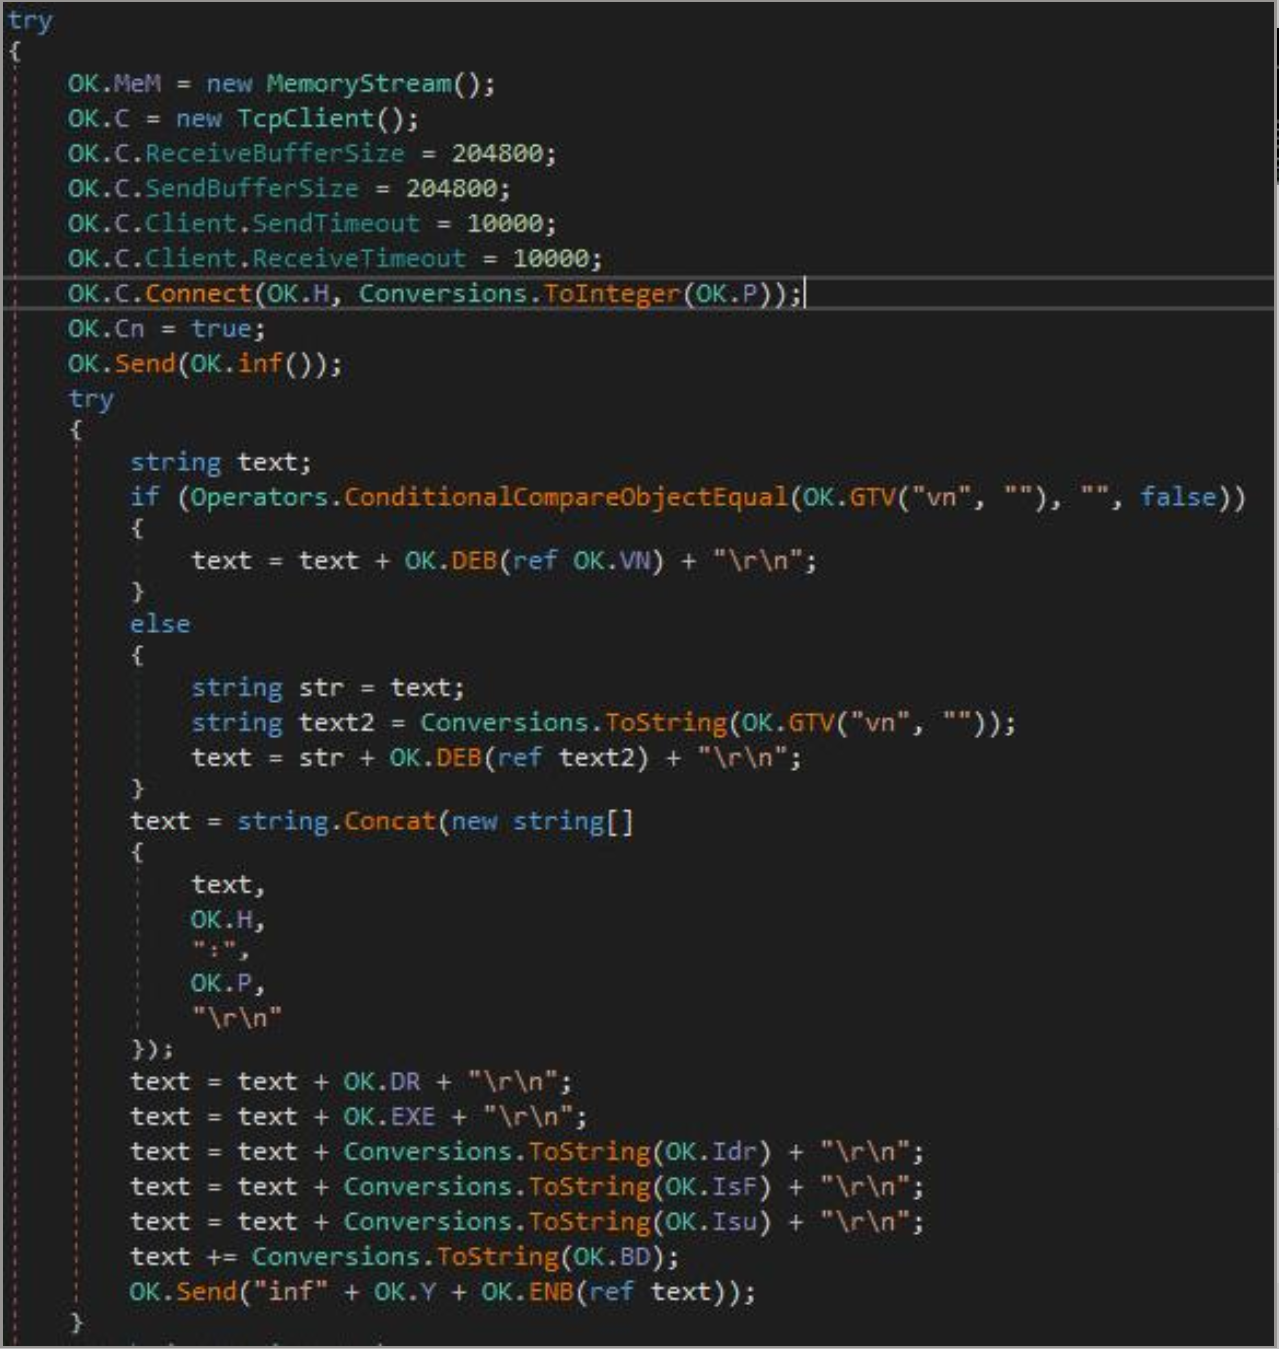
\includegraphics[width=6cm,keepaspectratio]{njrat_cnc}
      \caption{NJRat - CnC Decompiled Code}
    \end{figure}
  \end{center}
\end{frame}

\begin{frame}
  \frametitle{Analysis from Threat Intelligence}
  \framesubtitle{A Day in the Life 22 - Analysis from Threat Intelligence}
  \begin{center}
    \begin{figure}
      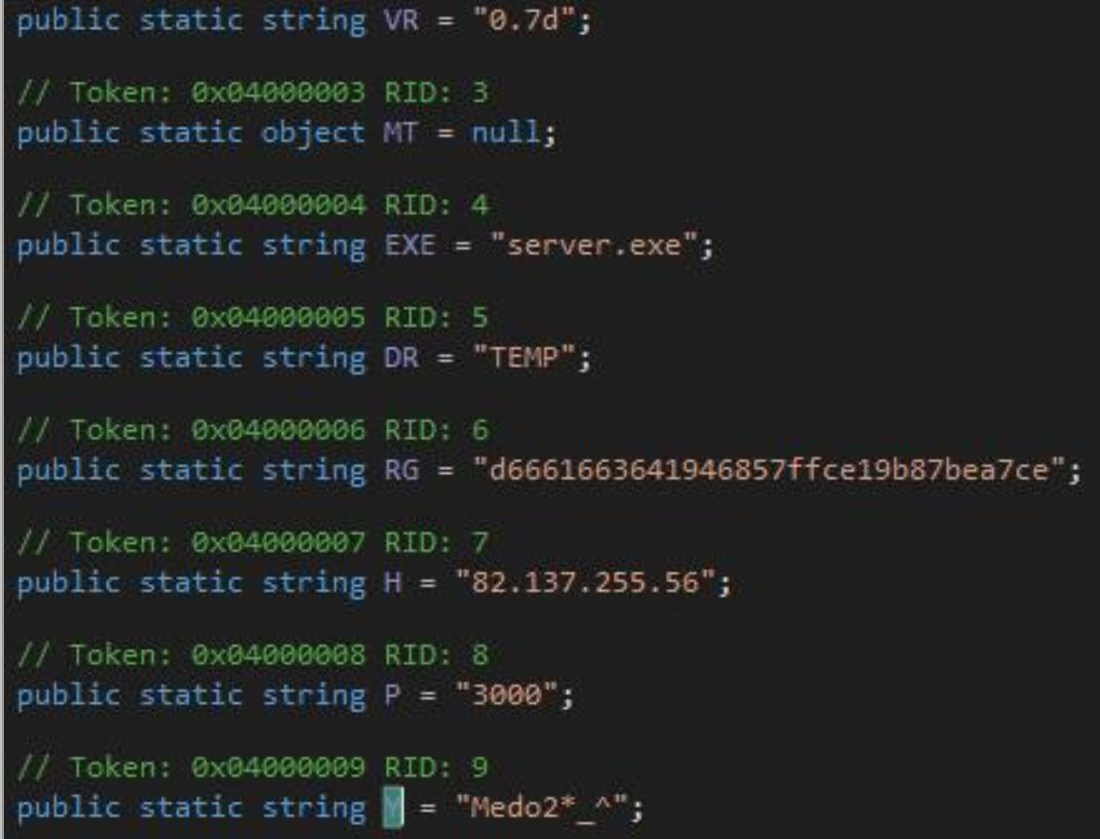
\includegraphics[width=8cm,keepaspectratio]{njrat_strings}
      \caption{NJRat - Helpful Strings}
    \end{figure}
  \end{center}
\end{frame}

\begin{frame}
  \frametitle{Analysis from Threat Intelligence}
  \framesubtitle{A Day in the Life 23 - Analysis from Threat Intelligence}
  \begin{center}
    \begin{figure}
      
\includegraphics[width=8cm,keepaspectratio]{powerpool_meme}
      \caption{PowerPool Malware}
    \end{figure}
  \end{center}
\end{frame}

\begin{frame}
  \frametitle{Analysis from Threat Intelligence}
  \framesubtitle{A Day in the Life 24 - Analysis from Threat Intelligence}
  \begin{center}
    \begin{figure}
      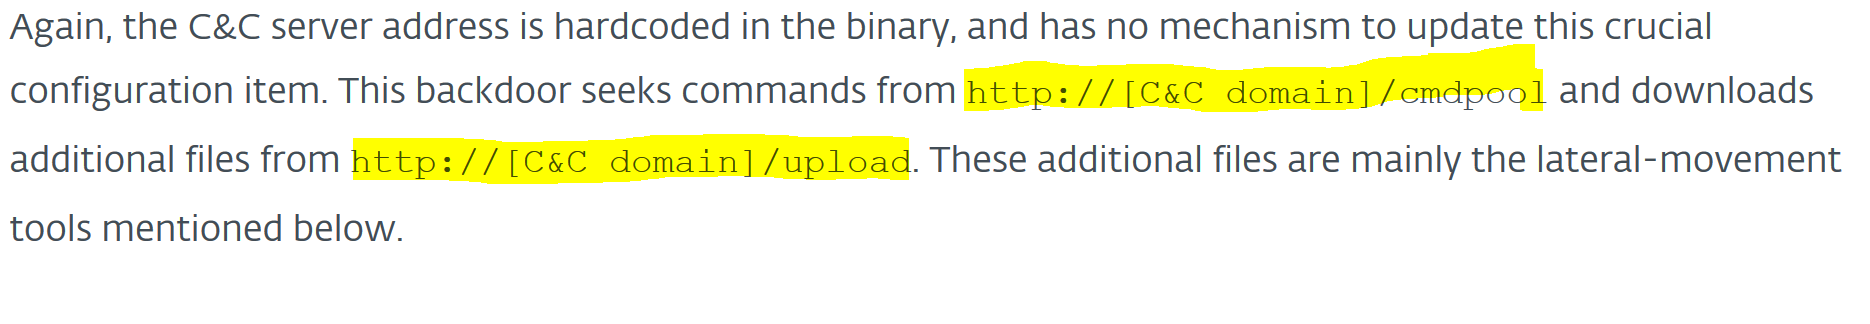
\includegraphics[width=14cm,keepaspectratio]{powerpool_article}
      \caption{PowerPool Malware}
    \end{figure}
  \end{center}
\end{frame}

\begin{frame}
  \frametitle{Analysis from Threat Intelligence}
  \framesubtitle{A Day in the Life 25 - Analysis from Threat Intelligence}
  \begin{center}
    \begin{figure}
      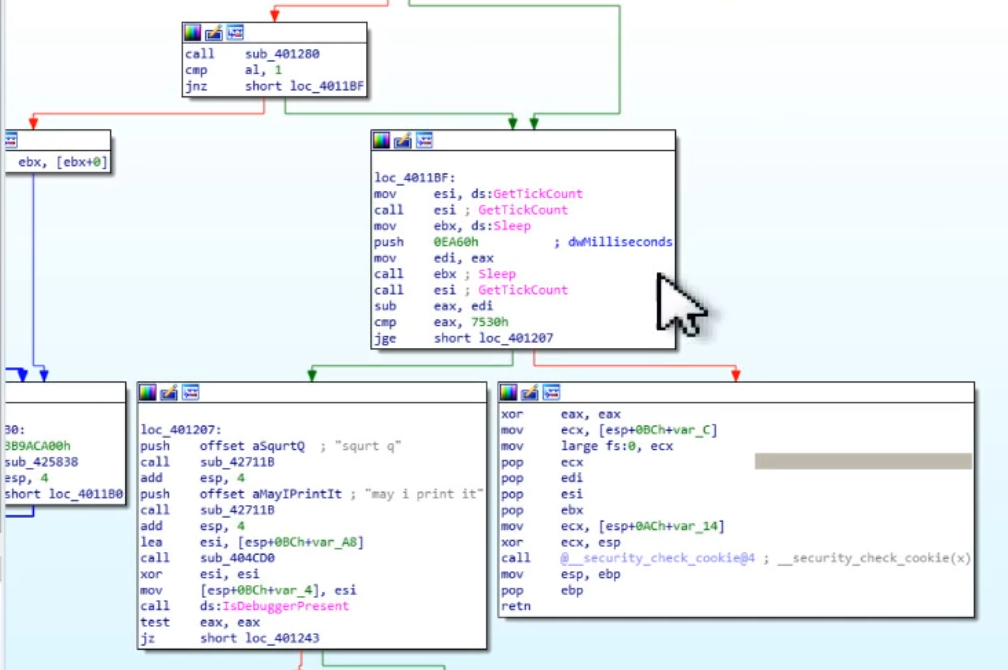
\includegraphics[width=9cm,keepaspectratio]{powerpool_anti_debug}
      \caption{PowerPool - Anti-Debugging}
    \end{figure}
  \end{center}
\end{frame}

\begin{frame}
  \frametitle{Analysis from Threat Intelligence}
  \framesubtitle{A Day in the Life 26 - Analysis from Threat Intelligence}
  \begin{center}
    \begin{figure}
      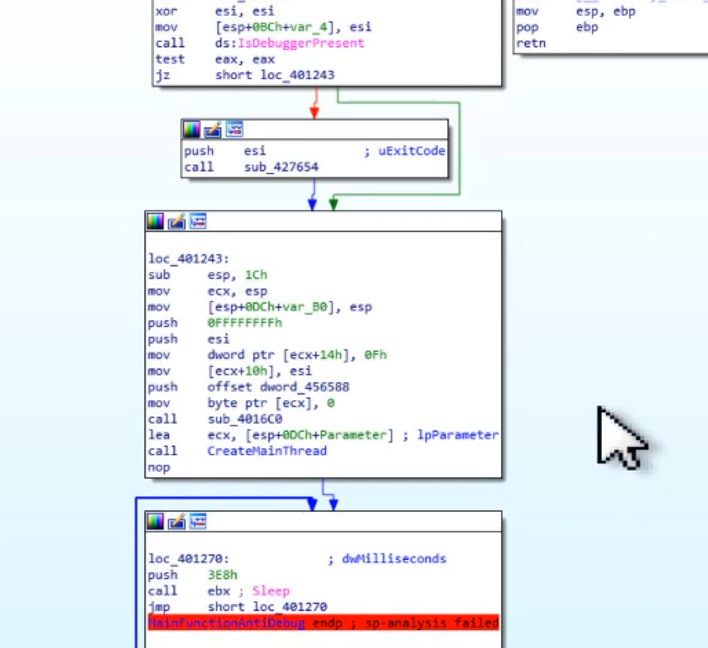
\includegraphics[width=6.5cm,keepaspectratio]{powerpool_main_thread}
      \caption{PowerPool - Main Thread}
    \end{figure}
  \end{center}
\end{frame}

\begin{frame}
  \frametitle{Afternoon}
  \framesubtitle{A Day in the Life 27 - Afternoon}
  \begin{columns}[onlytextwidth]
    \begin{column}{.30\textwidth}
      \begin{figure}
        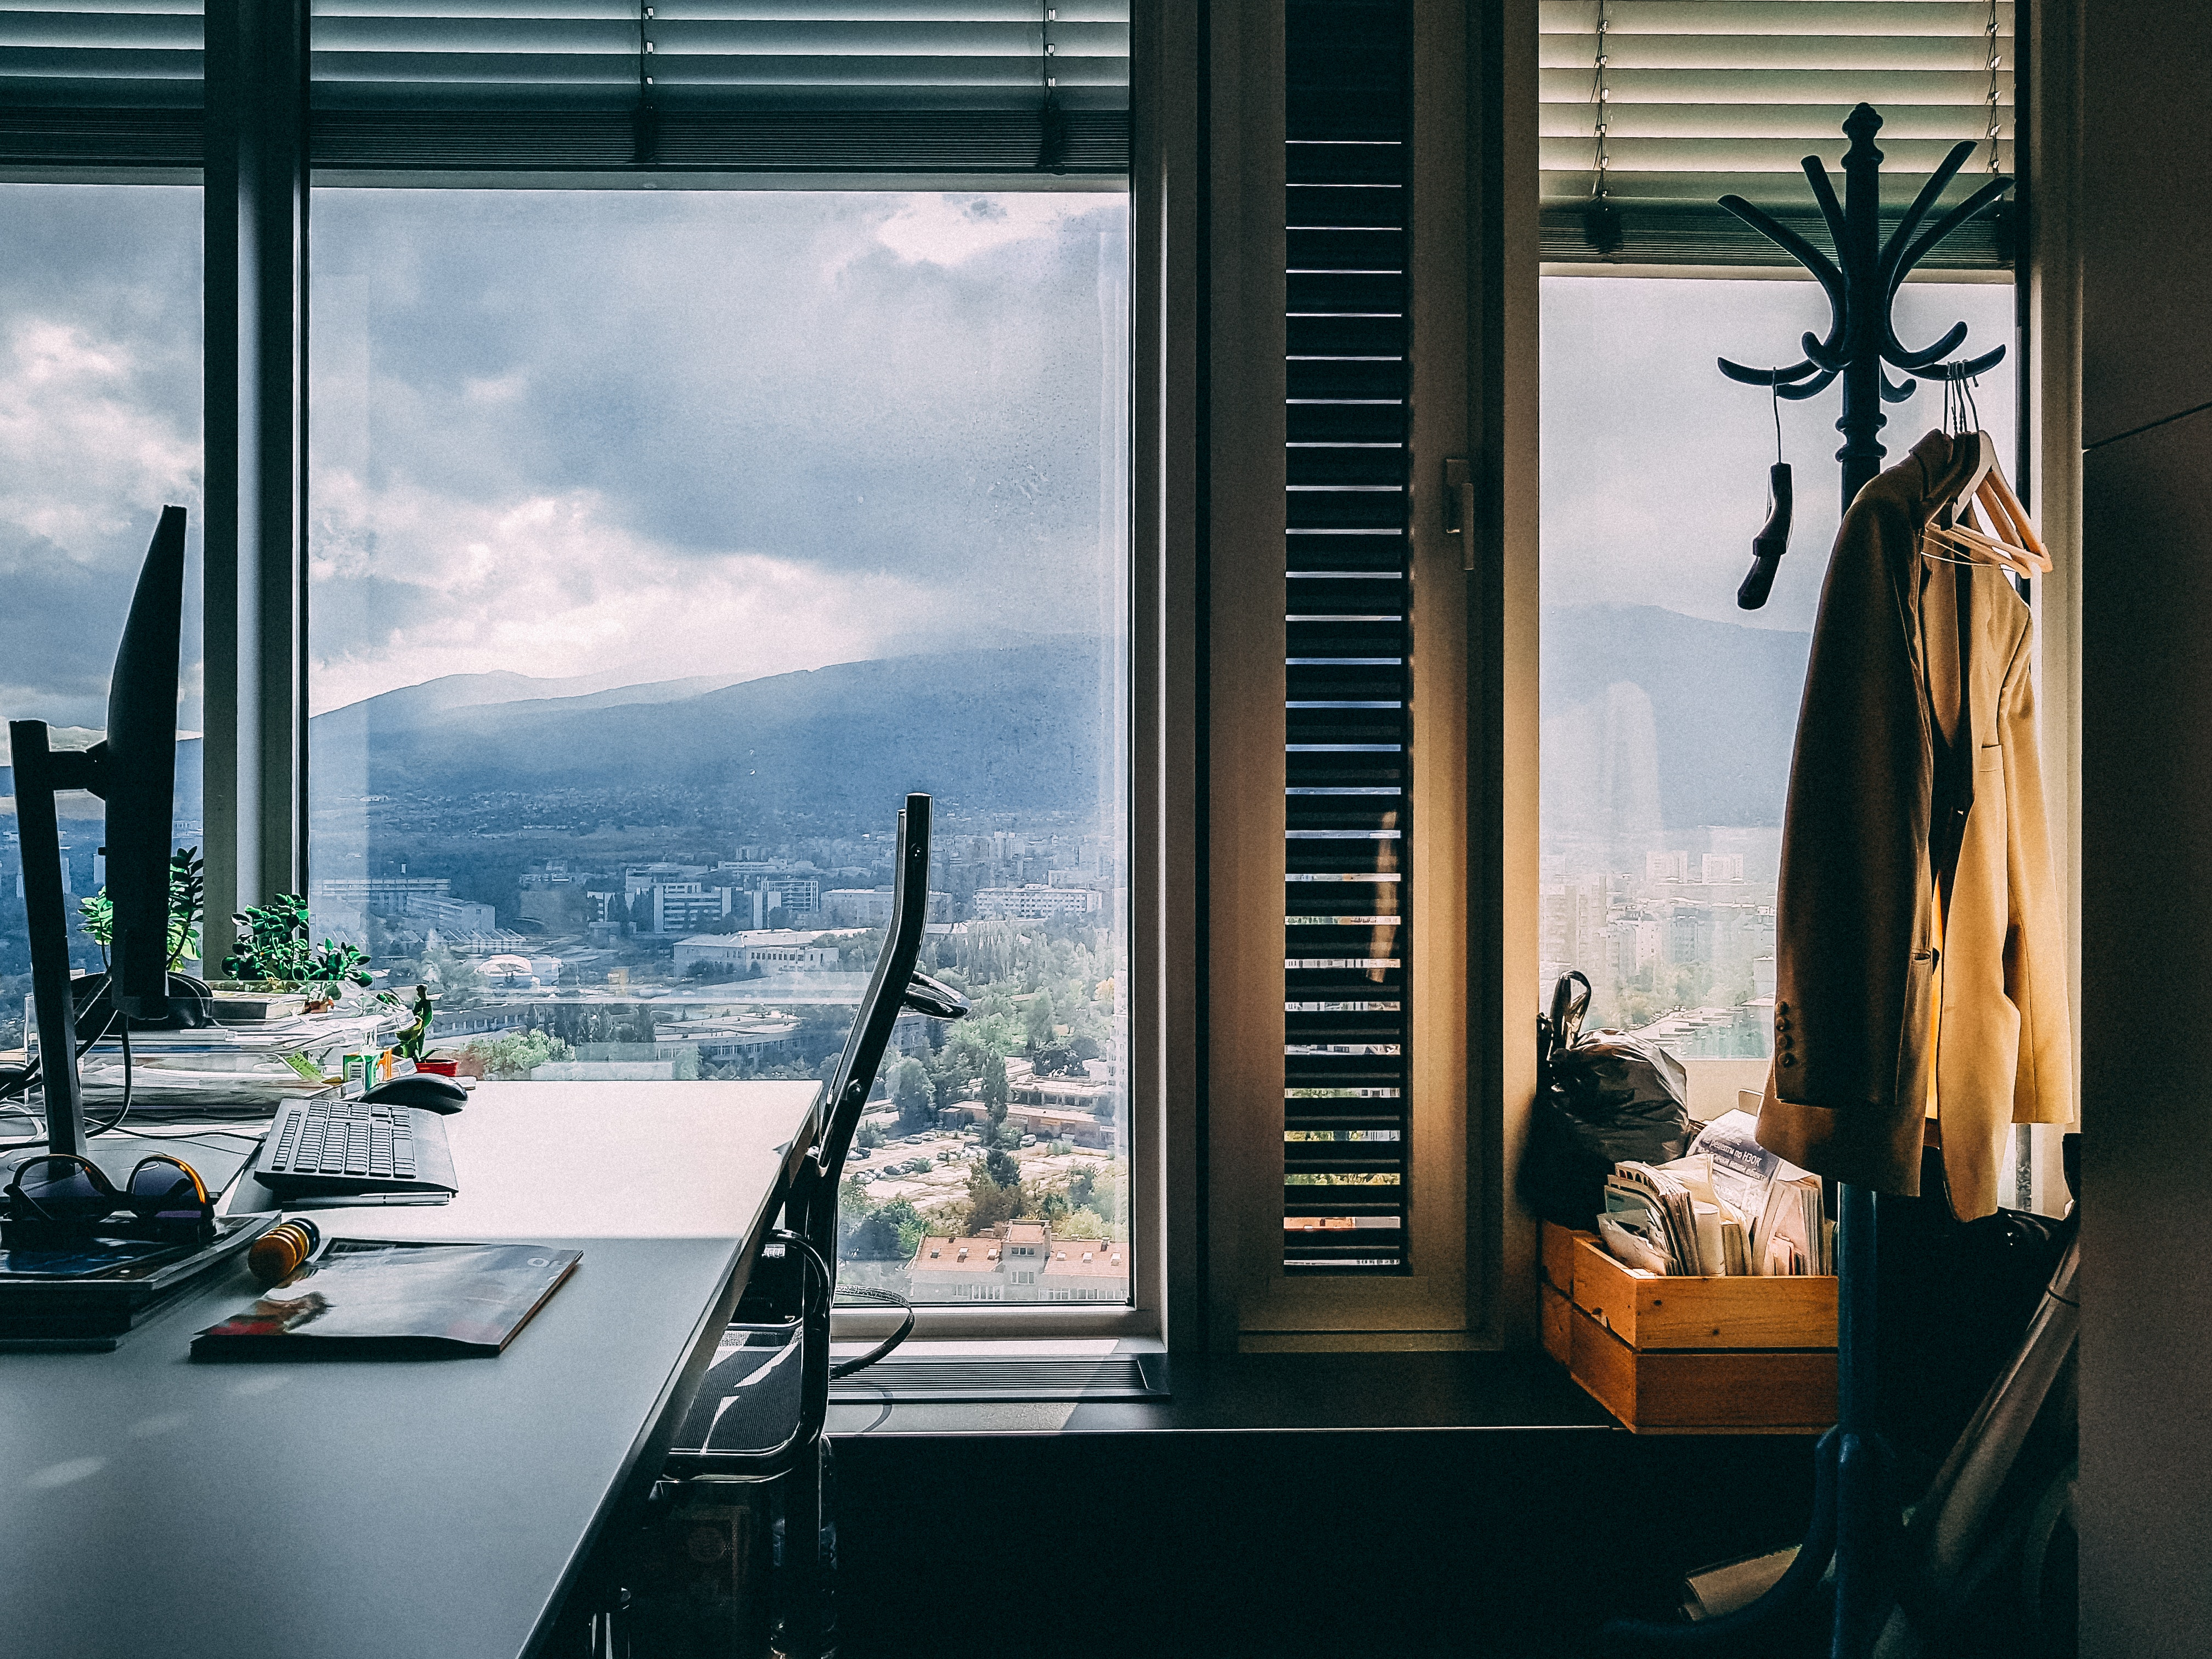
\includegraphics[width=5.5cm,keepaspectratio]{afternoon}
        \caption{Afternoon}
      \end{figure}
    \end{column}
    \hfill
    \begin{column}{.60\textwidth}
        \begin{tcolorbox}[title=programming.log,colback=gray]
         Programming Threat Intelligence API. Collecting malicious file hashes, urls, ip addresses, emails and more. 
        \end{tcolorbox}
    \end{column}
  \end{columns}
\end{frame}

\begin{frame}
  \frametitle{Travel}
  \framesubtitle{A Day in the Life 28 - Travel}
  \begin{columns}[onlytextwidth]
    \begin{column}{.30\textwidth}
      \begin{figure}
        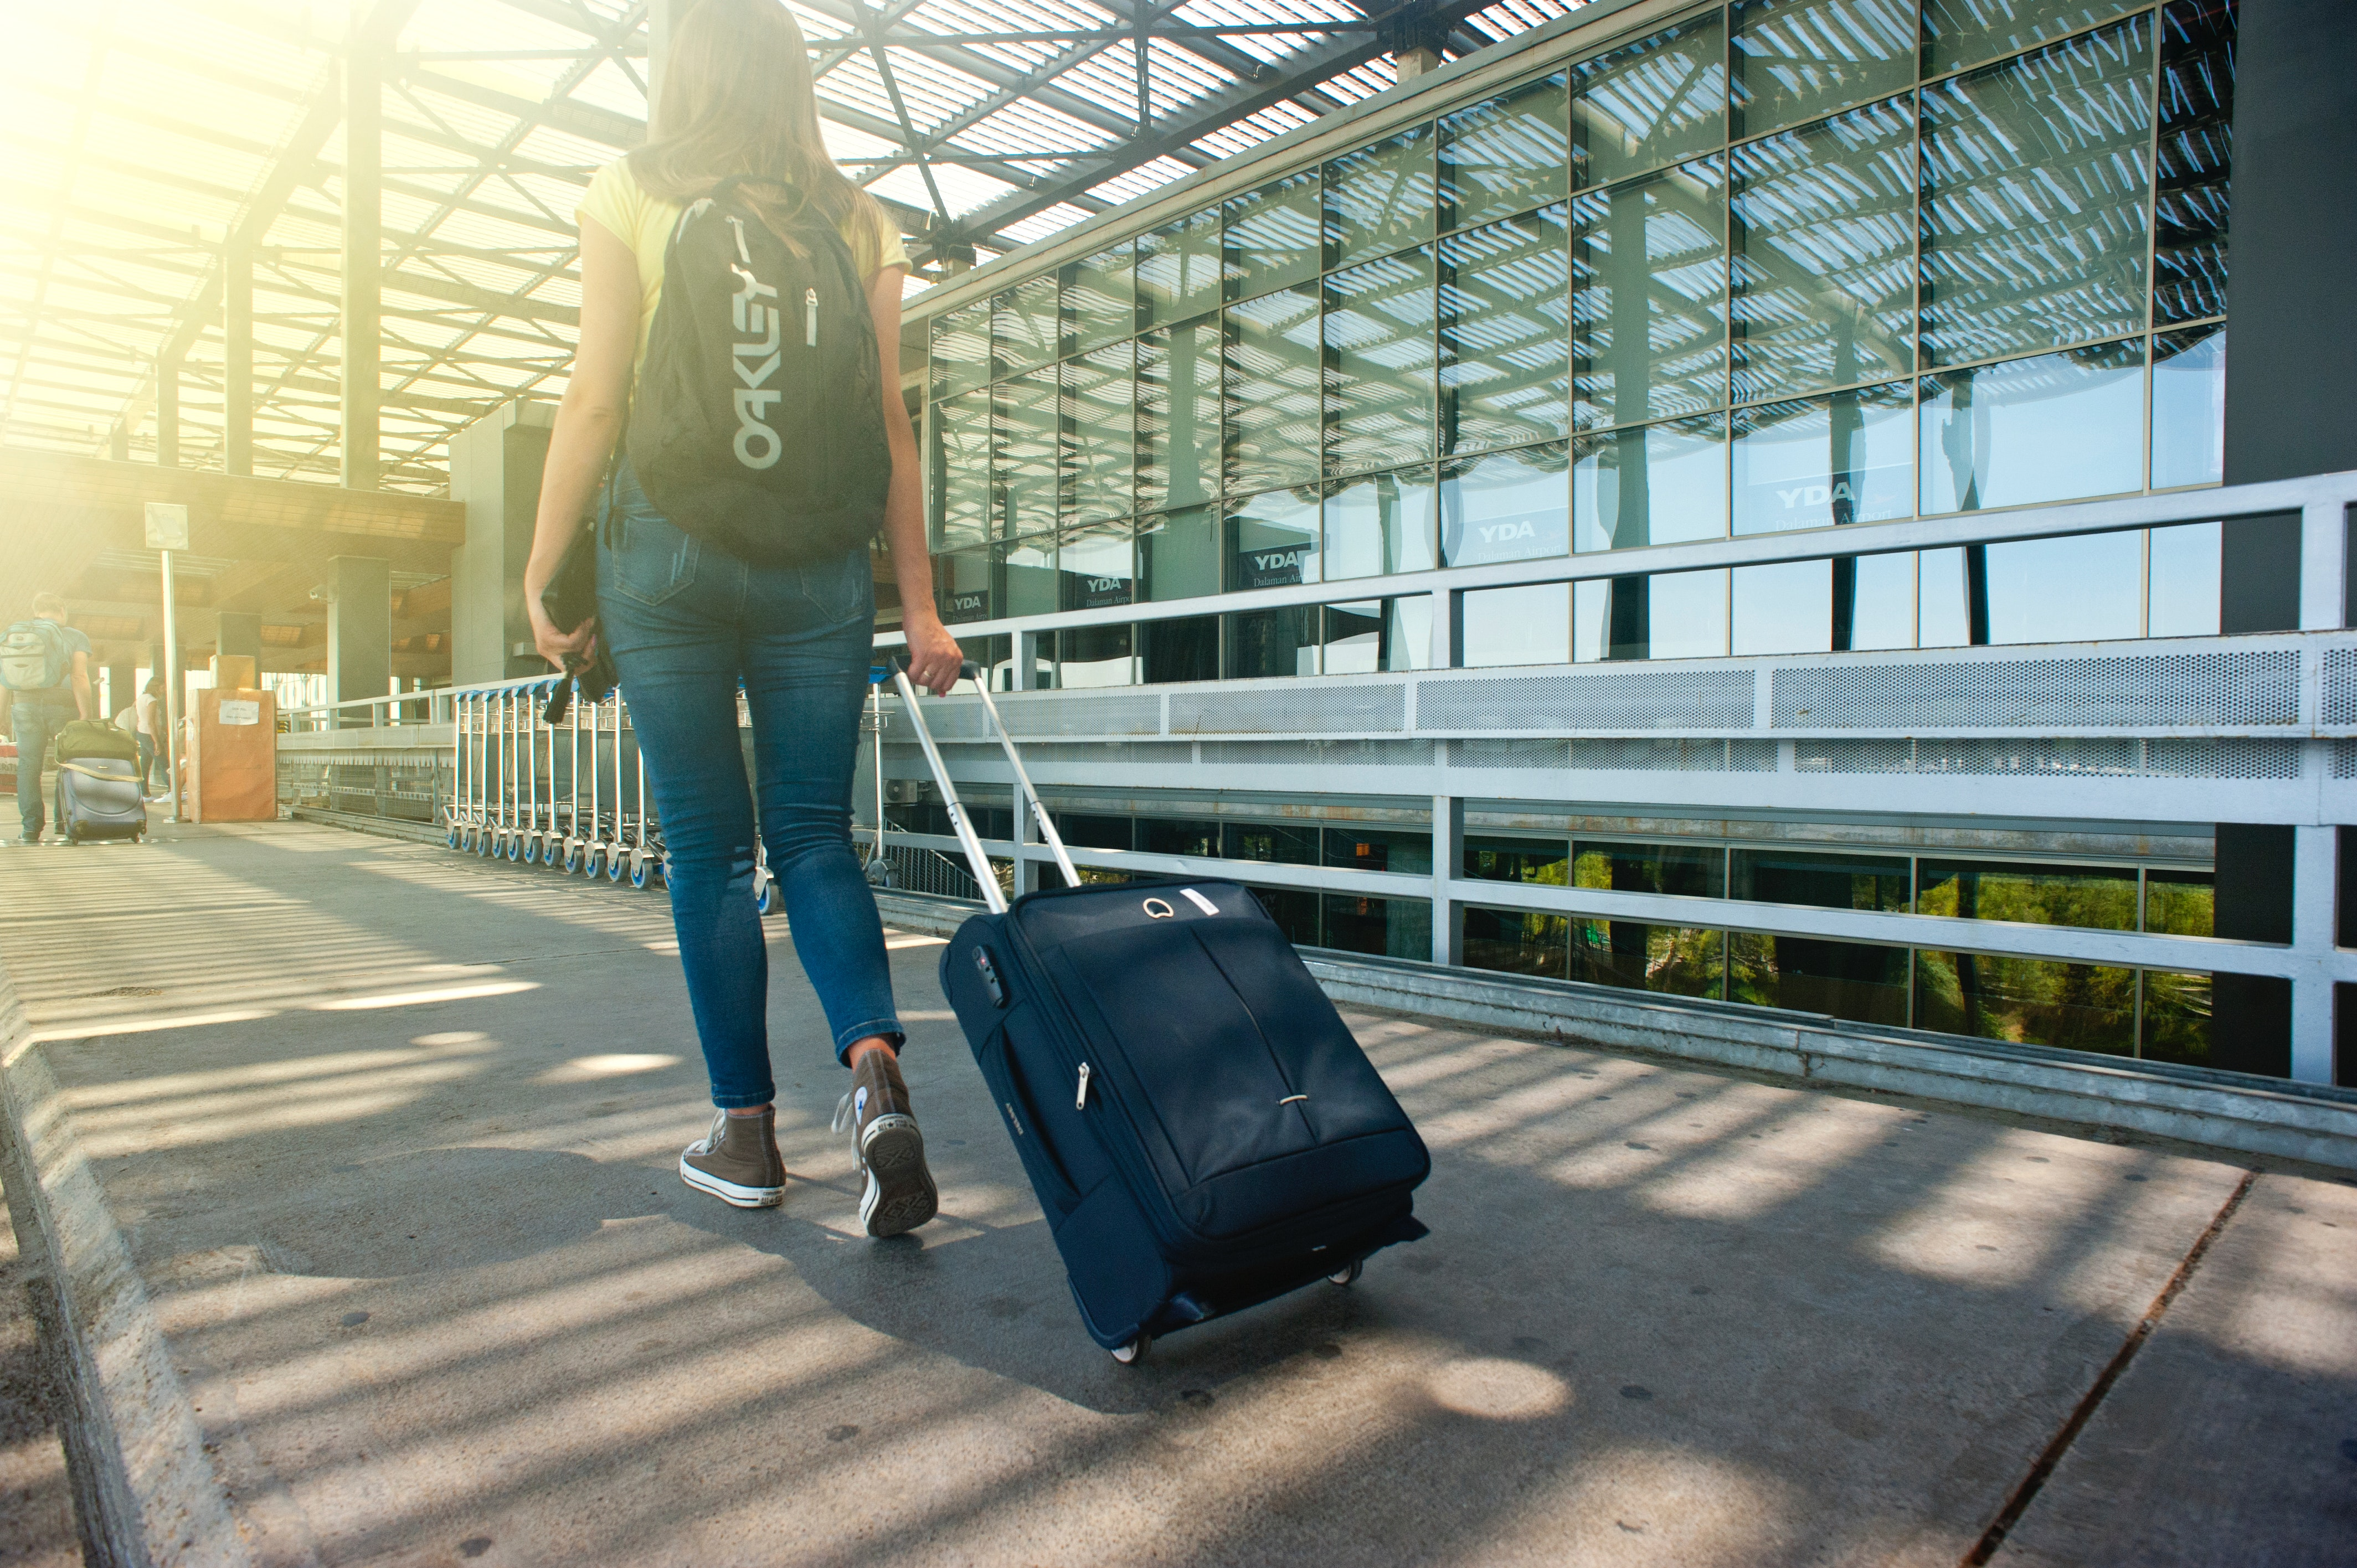
\includegraphics[width=5.5cm,keepaspectratio]{travel}
        \caption{Travel}
      \end{figure}
    \end{column}
    \hfill
    \begin{column}{.60\textwidth}
        \begin{tcolorbox}[title=travel.log,colback=gray]
          You can travel a lot in this industry if you have high quality information you can share at conferences. There are many call for papers that you can submit for. This will allow you to travel and present on what you are highly interested in.
        \end{tcolorbox}
    \end{column}
  \end{columns}
\end{frame}

\begin{frame}
  \frametitle{An Exciting Career}
  \framesubtitle{Why is it so exciting?}
  \begin{columns}[onlytextwidth]
    \begin{column}{.30\textwidth}
      \begin{figure}
        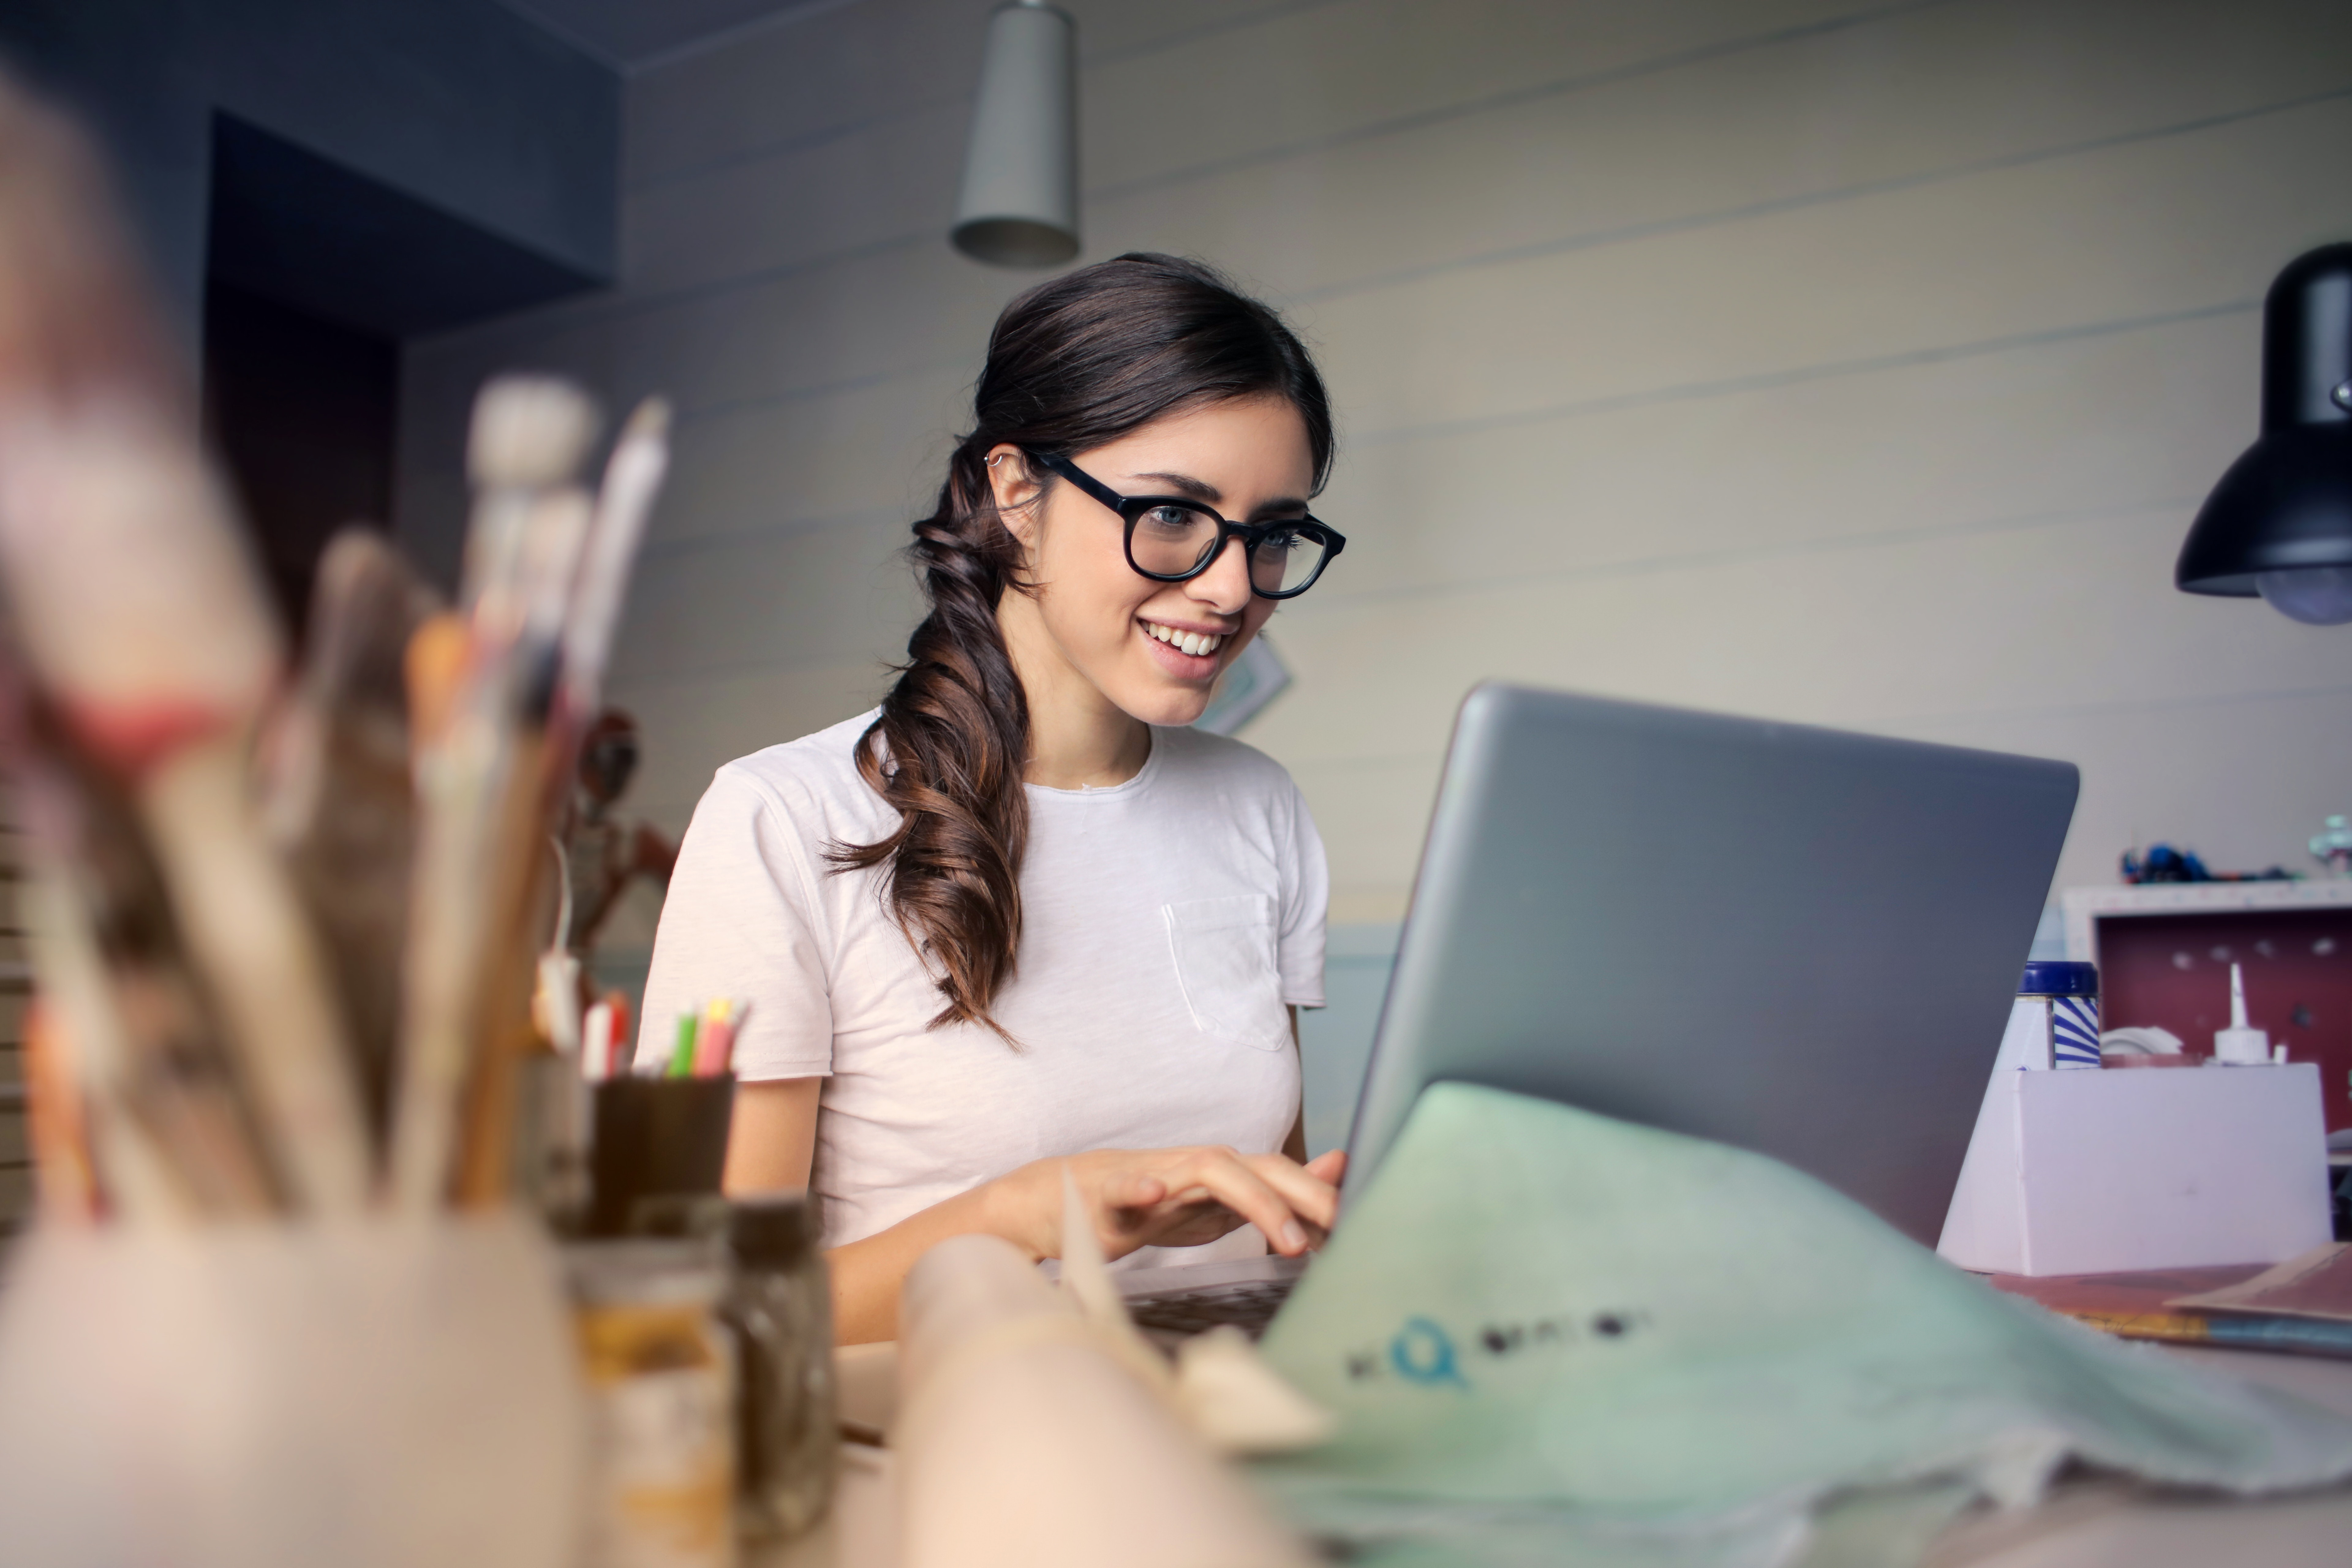
\includegraphics[width=5.5cm,keepaspectratio]{exciting}
        \caption{Exciting Carrer}
      \end{figure}
    \end{column}
    \hfill
    \begin{column}{.60\textwidth}
        \begin{tcolorbox}[title=exciting.log,colback=gray]
          Catching the bad guys, lots of opportunity currently available, competitive salaries, work from home sometimes, and much more!
        \end{tcolorbox}
    \end{column}
  \end{columns}
\end{frame}

\begin{frame}
  \frametitle{Summary}
  \begin{itemize}
  \item{Explore your Passions}
  \item{Find your Passion in Opportunities}
  \item{Try, Fail, Try Again, Succeed}
  \item{Show your Value}
  \item{Always keep Learning}
  \end{itemize}
\end{frame}

\begin{frame}
  \frametitle{Questions}
  \begin{center}
    \begin{figure}
      
\includegraphics[width=6cm,keepaspectratio]{questions_meme}
      \caption{I Love Questions}
    \end{figure}
  \end{center}
\end{frame}

\begin{frame}
  \frametitle{Can I Has Your Slides and Codes Plz?}
  \begin{center}
    \begin{figure}
      
\includegraphics[width=7cm,keepaspectratio]{git_meme}
      \caption{\href{https://github.com/lillypad/nscc-tech-connect}{https://github.com/lillypad/nscc-tech-connect}}
    \end{figure}
  \end{center}
\end{frame}

\begin{frame}
  \frametitle{References}
  \begin{center}
    \begin{itemize}
    \item{\href{https://en.wikipedia.org/wiki/Main_Page}{Wikipedia}}
    \item{\href{https://ti.360.net/blog/articles/analysis-of-apt-c-27/}{NJRat Article}}
    \item{\href{https://www.virustotal.com/\#/file/0a9c88d03260b92608c9c079a1b449cf46e5cd764f12f2ec852038dd6bd0fa97/detection}{NJRat Sample}}
    \item{\href{https://www.virustotal.com/\#/file/4e51a6779a7776055ebdeffe28d00e8866b2e722e3ccb6cba868cf8cdc86b1a3/detection}{NJRat Unpacked Sample}}
    \item{\href{http://sfkino.tistory.com/70}{Alibaba Malware Article}}
    \item{\href{https://www.virustotal.com/\#/file/d057088d0de3d920ea0939217c756274018b6e89cbfc74f66f50a9d27a384b09/detection}{Alibaba Malware Sample}}
    \item{\href{https://www.welivesecurity.com/2018/09/05/powerpool-malware-exploits-zero-day-vulnerability/}{PowerPool Malware Article}}
    \item{\href{https://www.virustotal.com/\#/file/58a50840c04cd15f439f1cc1b684e9f9fa22c0d64f44a391d9e2b1222e5cd6bd/details}{PowerPool Malware Sample}}
    \item{\href{https://www.virustotal.com/\#/file/9c08136b26ee5234c61a5d9e5a17afb15da35efc66514d2df5b53178693644c5/detection}{PowerPool Malware Sample Patched Version}}
    \item{\href{https://www.symantec.com/security-center/writeup/2018-092116-1134-99?om_rssid=sr-latestthreats30days\#technicaldescription}{FancyBear APT Article}}
    \item{\href{https://www.virustotal.com/\#/file/a37eda810ca92486bfb0e1f1b27adb7c9df57aafab686c000ae1d6ec5d6f6180/detection}{FancyBear APT Sample}}
    \item{\href{https://www.virustotal.com/\#/file/90e7c99effc7e4360c45a2af7ca9cc23313902a40c30d48cac8db048e9e4c0f6/detection}{FancyBear APT Unpacked .NET Assembly}}
    \end{itemize}
  \end{center}
\end{frame}

\end{document}
